%%%%%%%%%%%%%%%%%%%%%%%%%%%%%%%%%%%%%%%%%
% The Reissner-Nordström metric
% LaTeX tufte book
% Version 2.0 (12/02/21)
%
% Original authors:
% Ignacio Lembo Ferrari(lemboignacio98@gmail.com)
% Franco Cassinese (cassinesefranco@gmail.com)
% Angel Ramirez (angel.jrr2000@gmail.com)
%%%%%%%%%%%%%%%%%%%%%%%%%%%%%%%%%%%%%%%%

%% Unfortunately for the contents to contain
%% the "Parts" lines successfully, hyperref
%% needs to be disabled.
\documentclass[a4paper,nohyper,nobib]{tufte-book}
%%%%%%%%%%%%%%%%%%%%%%%%%%%%%%%%%%%%%%%%%
\usepackage{booktabs}
\usepackage[utf8]{inputenc}
\usepackage[spanish]{babel}
\usepackage{csquotes}
\usepackage{tikz}
\usepackage{fancyhdr}
\usepackage{blindtext}
\usepackage{subcaption}
\usepackage{hyperref}
\usepackage[shortlabels]{enumitem}
\usepackage{caption,amsfonts,epsfig,amsmath,amssymb,amsbsy,bm,multicol}
\usepackage{multirow}
\usepackage{media9}
%\usepackage[siunitx]{circuitikz}
%\usepackage[amsmath]{empheq}
\usepackage{epigraph}
\usepackage[T1]{fontenc}%%
\usepackage[shortlabels]{enumitem}
%\usepackage{verbatim}

\usepackage{nameref}
% \hypersetup{colorlinks}% uncomment this line if you prefer colored hyperlinks (e.g., for onscreen viewing)

% \usepackage{hyphenat}
\usepackage{url}
\usepackage[backend=biber, natbib=true, style=numeric]{biblatex}
\addbibresource{sample-handout.bib}
\usepackage{xargs}
\renewcommandx{\cite}[3][1={0pt},2={}]{\sidenote[][#1]{\fullcite[#2]{#3}}}

%%%%%%%%%%%%%%%%%%%%%%%%%%%%%%%%%%%%%%%%%%%
% Book metadata
\title{Agujeros Negros de Reissner-Nordström}
\date{Relatividad General}
\author[Franco Cassinese, Ignacio Lembo Ferrari, Angel Ramírez]{Franco Cassinese,\\ Ignacio Lembo Ferrari,\\ Angel Ramírez}
\publisher[]{UNIVERSIDAD NACIONAL DE ROSARIO\\
\bigskip
FACULTAD DE CIENCIAS EXACTAS, INGENIERÍA Y AGRIMENSURA\\
\bigskip
DEPARTAMENTO DE FÍSICA-ESCUELA DE CIENCIAS EXACTAS Y NATURALES
}
%%%%%%%%%%%%%%%%%%%%%%%%%%%%%%%%%%%%%%%%%%%%%%
%\usepackage{microtype}

%%
% For nicely typeset tabular material
%\usepackage{booktabs}

%%
% For graphics / images
\usepackage{graphicx}
\setkeys{Gin}{width=\linewidth,totalheight=\textheight,keepaspectratio}
\graphicspath{{graphics/}}



% Prints argument within hanging parentheses (i.e., parentheses that take
% up no horizontal space).  Useful in tabular environments.
\newcommand{\hangp}[1]{\makebox[0pt][r]{(}#1\makebox[0pt][l]{)}}

%%
% Prints an asterisk that takes up no horizontal space.
% Useful in tabular environments.
\newcommand{\hangstar}{\makebox[0pt][l]{*}}

%%
% Prints a trailing space in a smart way.
\usepackage{xspace}

%%
% Some shortcuts for Tufte's book titles.  The lowercase commands will
% produce the initials of the book title in italics.  The all-caps commands
% will print out the full title of the book in italics.
%\newcommand{\TL}{Tufte-\LaTeX\xspace}

% Prints an epigraph and speaker in sans serif, all-caps type.
\newcommand{\openepigraph}[2]{%
  %\sffamily\fontsize{14}{16}\selectfont
  \begin{fullwidth}
  \sffamily\large
  \begin{doublespace}
  \noindent\allcaps{#1}\\% epigraph
  \noindent\allcaps{#2}% author
  \end{doublespace}
  \end{fullwidth}
}

% Inserts a blank page
\newcommand{\blankpage}{\newpage\hbox{}\thispagestyle{empty}\newpage}

\usepackage{units}

% Typesets the font size, leading, and measure in the form of 10/12x26 pc.
\newcommand{\measure}[3]{#1/#2$\times$\unit[#3]{pc}}

% Macros for typesetting the documentation
\newcommand{\hlred}[1]{\textcolor{Maroon}{#1}}% prints in red
\newcommand{\hangleft}[1]{\makebox[0pt][r]{#1}}
\newcommand{\hairsp}{\hspace{1pt}}% hair space
\newcommand{\hquad}{\hskip0.5em\relax}% half quad space
\newcommand{\TODO}{\textcolor{red}{\bf !TODO}\xspace}
\newcommand{\ie}{\textit{i.\hairsp{}e.}\xspace}
\newcommand{\eg}{\textit{e.\hairsp{}g.}\xspace}
\newcommand{\na}{\quad--}% used in tables for N/A cells
\providecommand{\XeLaTeX}{X\lower.5ex\hbox{\kern-0.15em\reflectbox{E}}\kern-0.1em\LaTeX}
\newcommand{\tXeLaTeX}{\XeLaTeX\index{XeLaTeX@\protect\XeLaTeX}}
% \index{\texttt{\textbackslash xyz}@\hangleft{\texttt{\textbackslash}}\texttt{xyz}}
\newcommand{\tuftebs}{\symbol{'134}}% a backslash in tt type in OT1/T1
\newcommand{\doccmdnoindex}[2][]{\texttt{\tuftebs#2}}% command name -- adds backslash automatically (and doesn't add cmd to the index)
\newcommand{\doccmddef}[2][]{%
  \hlred{\texttt{\tuftebs#2}}\label{cmd:#2}%
  \ifthenelse{\isempty{#1}}%
    {% add the command to the index
      \index{#2 command@\protect\hangleft{\texttt{\tuftebs}}\texttt{#2}}% command name
    }%
    {% add the command and package to the index
      \index{#2 command@\protect\hangleft{\texttt{\tuftebs}}\texttt{#2} (\texttt{#1} package)}% command name
      \index{#1 package@\texttt{#1} package}\index{packages!#1@\texttt{#1}}% package name
    }%
}% command name -- adds backslash automatically
\newcommand{\doccmd}[2][]{%
  \texttt{\tuftebs#2}%
  \ifthenelse{\isempty{#1}}%
    {% add the command to the index
      \index{#2 command@\protect\hangleft{\texttt{\tuftebs}}\texttt{#2}}% command name
    }%
    {% add the command and package to the index
      \index{#2 command@\protect\hangleft{\texttt{\tuftebs}}\texttt{#2} (\texttt{#1} package)}% command name
      \index{#1 package@\texttt{#1} package}\index{packages!#1@\texttt{#1}}% package name
    }%
}% command name -- adds backslash automatically
\newcommand{\docopt}[1]{\ensuremath{\langle}\textrm{\textit{#1}}\ensuremath{\rangle}}% optional command argument
\newcommand{\docarg}[1]{\textrm{\textit{#1}}}% (required) command argument
\newenvironment{docspec}{\begin{quotation}\ttfamily\parskip0pt\parindent0pt\ignorespaces}{\end{quotation}}% command specification environment
\newcommand{\docenv}[1]{\texttt{#1}\index{#1 environment@\texttt{#1} environment}\index{environments!#1@\texttt{#1}}}% environment name
\newcommand{\docenvdef}[1]{\hlred{\texttt{#1}}\label{env:#1}\index{#1 environment@\texttt{#1} environment}\index{environments!#1@\texttt{#1}}}% environment name
\newcommand{\docpkg}[1]{\texttt{#1}\index{#1 package@\texttt{#1} package}\index{packages!#1@\texttt{#1}}}% package name
\newcommand{\doccls}[1]{\texttt{#1}}% document class name
\newcommand{\docclsopt}[1]{\texttt{#1}\index{#1 class option@\texttt{#1} class option}\index{class options!#1@\texttt{#1}}}% document class option name
\newcommand{\docclsoptdef}[1]{\hlred{\texttt{#1}}\label{clsopt:#1}\index{#1 class option@\texttt{#1} class option}\index{class options!#1@\texttt{#1}}}% document class option name defined
\newcommand{\docmsg}[2]{\bigskip\begin{fullwidth}\noindent\ttfamily#1\end{fullwidth}\medskip\par\noindent#2}
\newcommand{\docfilehook}[2]{\texttt{#1}\index{file hooks!#2}\index{#1@\texttt{#1}}}
\newcommand{\doccounter}[1]{\texttt{#1}\index{#1 counter@\texttt{#1} counter}}

% Generates the index
\usepackage{makeidx}
\makeindex

%%%% Kevin Godny's code for title page and contents from https://groups.google.com/forum/#!topic/tufte-latex/ujdzrktC1BQ
\usepackage{pdfpages}
\makeatletter
\renewcommand{\maketitlepage}{%
\begingroup%
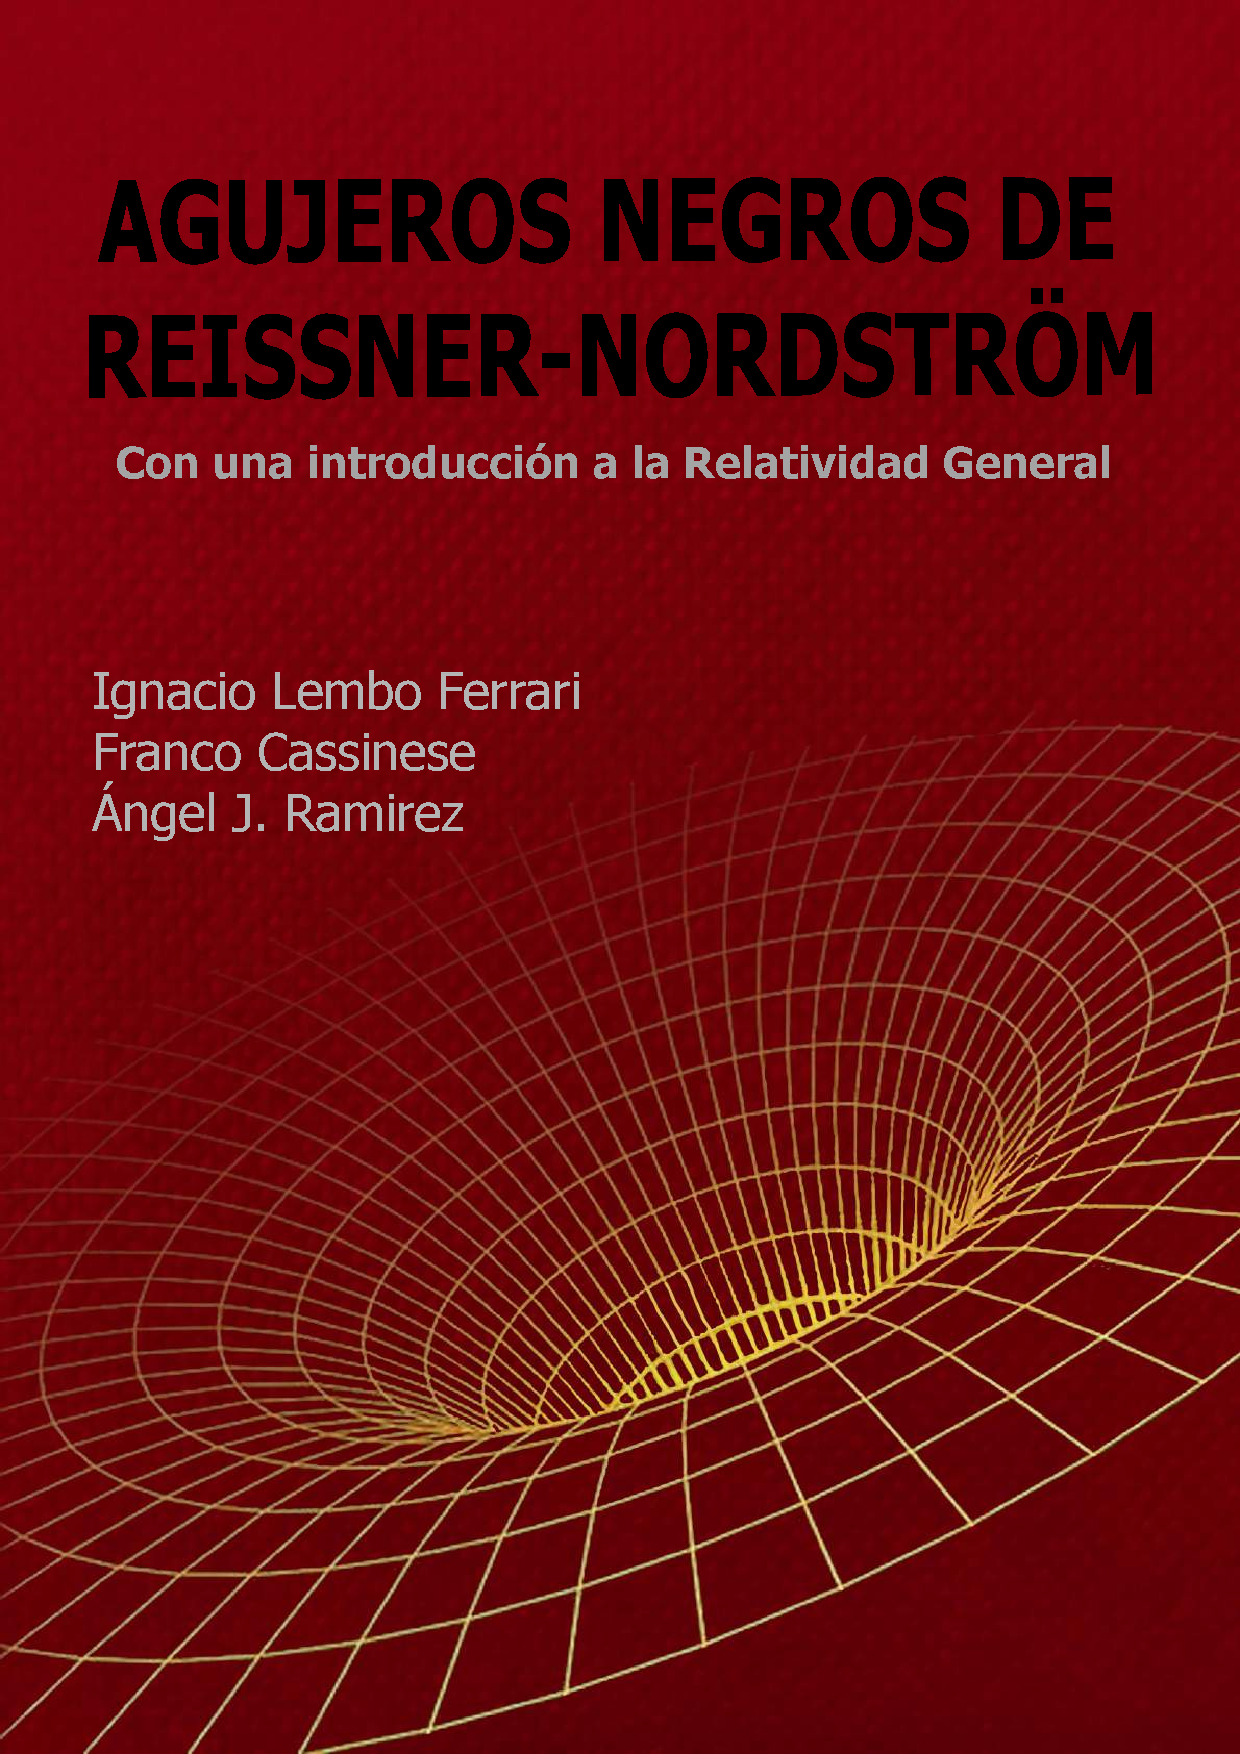
\includepdf[pages=1,fitpaper]{cover1}
\thispagestyle{empty}
\endgroup
}
\makeatother
%%%%%%%%%%%%%%%%%%%%%%%%%%%%%%%%%%%
%COPYRIGHT - Franco Cassinese, Angel Ramírez & Ignacio Lembo Ferrari UNR% 
%%%%%%%%%%%%%%%%%%%%%%%%%%%%%%%%%%%%
%Cajas de colores
\usepackage[many]{tcolorbox}
\usetikzlibrary{calc}

%Definicion de colores
\definecolor{myred}{RGB}{203,72,41}
\definecolor{mygreen}{rgb}{0.55,0.95,0.70}
\definecolor{darkgreen}{RGB}{1,108,10}

\tcbset{mystyle/.style={
  breakable,
  enhanced,
  outer arc=0pt,
  arc=0pt,
  colframe=darkgreen,
  colback=mygreen,
  coltitle=black,
  attach boxed title to top left,
  boxed title style={
    colback=mygreen,
    outer arc=0pt,
    arc=0pt,
    top=3pt,
    bottom=2pt,
    },
  fonttitle=\sffamily
  }
}
%%Cajas para resultados importantes
\newtcolorbox[auto counter]{resultados}[1][]{
  mystyle,
  title=Resultado~\thetcbcounter,
  overlay unbroken and first={
      \path
        let
        \p1=(title.north east),
        \p2=(frame.north east)
        in
        node[anchor=west,font=\sffamily,color=mygreen,text width=\x2-\x1] 
        at (title.east) {#1};
  }
}
%%Cajas para remarcar cosas que son importantes porque pueden servir despues o son conceptos que queremos que queden
\newtcolorbox{remarkbox}[2][]{
    title=Remark Box~\thetcbcounter,
    lower separated=false,
    colback=myred!20,
    colframe=myred,fonttitle=\bfseries,
    colbacktitle=myred!80,
    coltitle=black,
    enhanced,
    attach boxed title to top left=
    {xshift=0.5cm,yshift=-2mm},
    title=#2,#1
}
%%Cajas para añadir data extra que puede ser opcional de leer
\newtcolorbox{extrabox}[2][]{
    title=Extradata~\thetcbcounter,
    lower separated=false,
    colback=myred!50,
    arc=0pt,
    colframe=myred,fonttitle=\bfseries,
    colbacktitle=myred!50,
    coltitle=white,
    enhanced,
    attach boxed title to top left=
    {xshift=0.5cm,yshift=-2mm},
    title=#2,#1
}
%%%%%%%%%%%%%%%%%%%%%%%%%%%%%%%%%%%%%%%
%Chapter style
\usepackage{xcolor} % for colour
\setcounter{secnumdepth}{2}

%Options: Sonny, Lenny, Glenn, Conny, Rejne, Bjarne, Bjornstrup
\usepackage[T1]{fontenc}
\usepackage[Bjornstrup]{fncychap}
\ChNumVar{\fontsize{76}{80}\usefont{OT1}{ptm}{m}{n}\selectfont\textcolor{myred}}
\ChTitleVar{\raggedleft\Huge\sffamily\bfseries}


%%%%%%%%%%%%%%%%%%%%%%%%%%%%%%%%%%%%%%%%%
%Section style
\def\chpcolor{myred!90}
\def\chpcolortxt{myred!90}
\def\sectionfont{\sffamily\LARGE}
\makeatletter

\def\@sectionstrut{\vrule\@width\z@\@height12.5\p@}
\def\@makesectionhead#1{%
  {\par\vspace{20pt}%
   \parindent 0pt\raggedleft\sectionfont
   \colorbox{\chpcolor}{%
     \parbox[t]{90pt}{\color{white}\@sectionstrut\@depth4.5\p@\hfill
       \ifnum\c@secnumdepth>\z@\thesection\fi}%
   }%
   \begin{minipage}[t]{\dimexpr\textwidth-90pt-2\fboxsep\relax}
   \color{\chpcolortxt}\@sectionstrut\hspace{5pt}#1
   \end{minipage}\par
   \vspace{10pt}%
  }
}
\def\section{\@afterindentfalse\secdef\@section\@ssection}
\def\@section[#1]#2{%
  \ifnum\c@secnumdepth>\m@ne
    \refstepcounter{section}%
    \addcontentsline{toc}{section}{\protect\numberline{\thesection}#1}%
  \else
    \phantomsection
    \addcontentsline{toc}{section}{#1}%
  \fi
  \sectionmark{#1}%
  \if@twocolumn
    \@topnewpage[\@makesectionhead{#2}]%
  \else
    \@makesectionhead{#2}\@afterheading
  \fi
}
\def\@ssection#1{%
  \if@twocolumn
    \@topnewpage[\@makesectionhead{#1}]%
  \else
    \@makesectionhead{#1}\@afterheading
  \fi
}
\makeatother
%%%%%%%%%%%%%%%%%%%%%%%%%%%%%%%%%%%%%%%%%%%%%%
\hypersetup{
    colorlinks=true,
    linkcolor=red,
    filecolor=magenta,      
    urlcolor=violet,
    citecolor=magenta,
}

%----------------------------------------------------------------------------------------
%	BEGINNING OF DOCUMENT
%----------------------------------------------------------------------------------------

\begin{document}

\frontmatter

\maketitle

\mainmatter

\chapter{\textcolor{myred}{Distribución binomial}}

\section{\huge{Introducción}}

\textcolor{myred}{\hrule}

\newthought{Consideremos}, una población de individuos que no se reproducen y evolucionan en tiempo discreto que evolucionan en tiempo discreto. A cada paso de tiempo cada uno de ellos puede morir con probabilidad $d$. Calcule numéricamente la distribución de probabilidad de la población en función del tiempo (para algunos tiempos, y para un par de valores de d). Compare con la distribución
binomial exacta

Realizamos simulaciones 














\begin{marginfigure}
\captionsetup{type=figure}
    \centering
    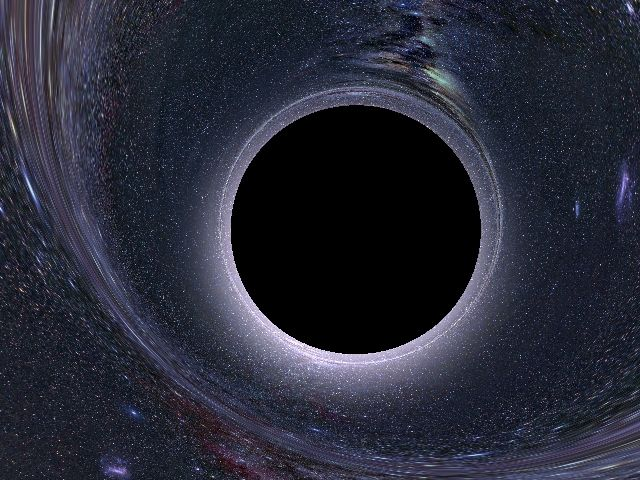
\includegraphics[width=1.3\textwidth]{Im/3653b705a42ad6a980fc834e6ca39875.jpg}
    \caption{Agujero negro de Reissner-Nordström, imagen generada por raytracing.}
    \label{fig:sen}
\end{marginfigure}

Es decir que, para cuando hallamos terminado el trabajo, tanto nosotrxs como lx lectorx deberá tener, al menos, una respuesta básica para las siguientes preguntas: ¿En qué consiste la Teoría General de la Relatividad?, ¿qué es la gravedad?, ¿qué es una métrica o un tensor métrico?, ¿qué significa que el espacio-tiempo esté 'curvado', y cómo puedo calcular dicha curvatura?, ¿cómo interviene la carga eléctrica en dicha curvatura?, ¿cómo son las trayectorias de partículas (neutras y cargadas) y de la luz, en un espacio-tiempo donde hay objetos con masa y carga eléctrica?
\begin{marginfigure}
\captionsetup{type=figure}
    \centering
    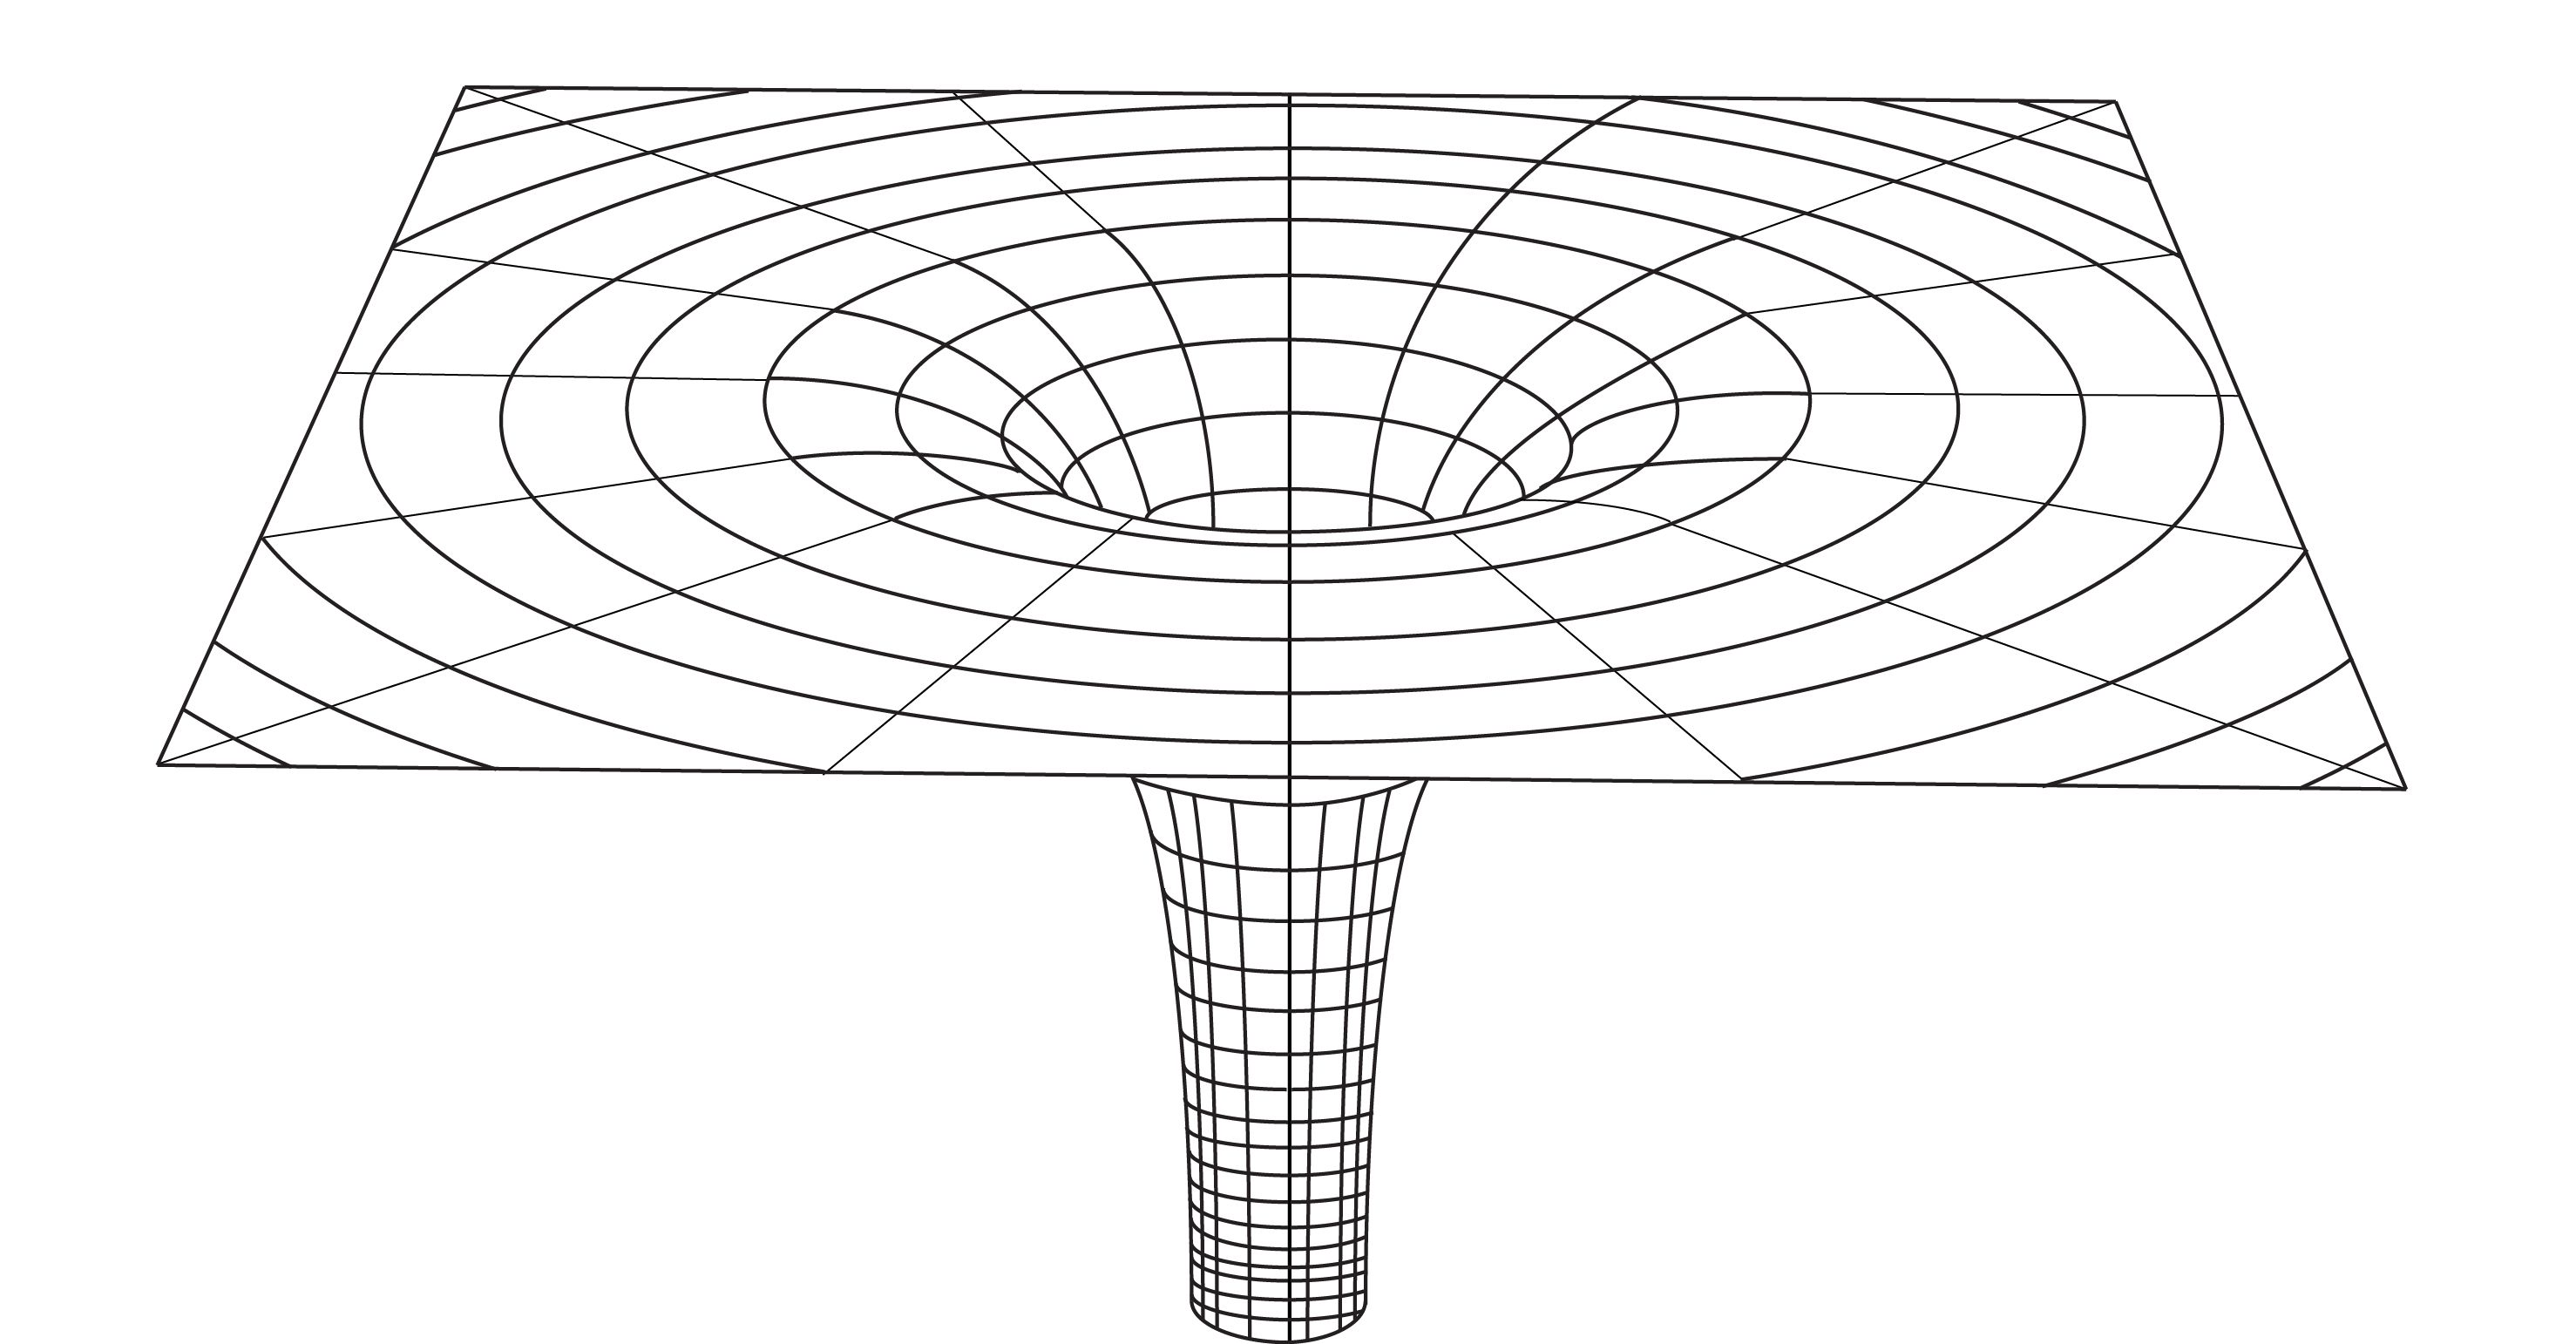
\includegraphics[width=1.3\textwidth]{Im/27c518672e8aa2b372107cca7726603f.jpg}
    \caption{Representación de un agujero negro.}
    \label{fig:sen}
\end{marginfigure}
Como siempre, es conveniente separar el trabajo en partes, y eso es lo que haremos aquí. Este documento consta entonces de cuatro capítulos y un epílogo:

\begin{remarkbox}{}
\begin{itemize}
    \item \textbf{Capítulo 1} - Teoría General de la Relatividad
    \item \textbf{Capítulo 2} - Ecuación de Campo de Einstein
    \item \textbf{Capítulo 3} - Métrica de Reissner-Nordström
    \item \textbf{Capítulo 4} - Simulaciones Computacionales
    \item \textbf{Epílogo} - Conclusiones, Fronteras y Bilbiografía
\end{itemize}
\end{remarkbox}

\section{\huge{GR in a nutshell}}
\textcolor{myred}{\hrule width\textwidth}

\begin{flushright}
\textit{Gravity is matter's response to loneliness.}\\ \textbf{Alice Wu}
\end{flushright}
\newthought{Sin más preámbulo}, comencemos \textit{spoileando} la Teoría General de la Relatividad (GR, por sus siglas en inglés). Para motivarnos, veamos primero la \textbf{Ley de Gravitación Universal} (Newton, 1687):

\begin{marginfigure}
\captionsetup{type=figure}
    \centering
    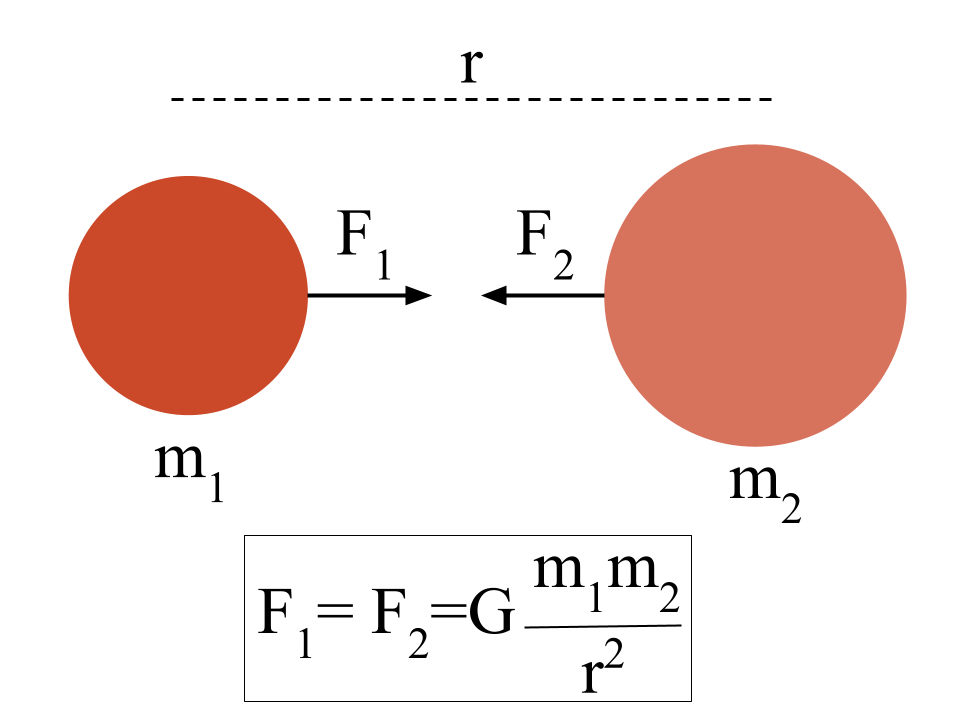
\includegraphics[width=1.3\textwidth]{Im/gravuniv.png}
    \caption{Ley de Gravitación Universal.}
    \label{fig:sen}
\end{marginfigure}

\begin{equation}
    F_{g}=G\frac{m_1 m_2}{r^2}
\end{equation}

Quien halla estudiado algo sobre la Teoría Especial de la Relatividad (SR), o esté familiarizadx con el fenómeno de \textbf{Retardación} del Electromagnetismo \footnote{\textbf{Retardation}, Cassinese F. y Lembo I. (2020)}, notará enseguida que esta ecuación no puede ser la explicación completa de la interacción gravitatoria: \textbf{el tiempo no aparece en ninguna parte}. Es decir que, por ejemplo, un cambio en la masa $m_1$ influiría \textbf{instantáneamente} en la masa $m_2$, y ya sabemos que en el mundo real casi nada es instantáneo. Claramente le falta algo a la teoría de Newton: explicar qué es la gravedad, cuál es el mecanismo según el cual los objetos con masa interactúan entre sí.

\newthought{Ahora bien,} ¿cuál es este mecanismo? Para dar con él, vamos a establecer dos relaciones fundamentales: primero, la \textbf{relación entre gravedad y aceleración}, y luego la \textbf{relación entre aceleración y curvatura}.


\begin{figure}[h!]
    \centering
    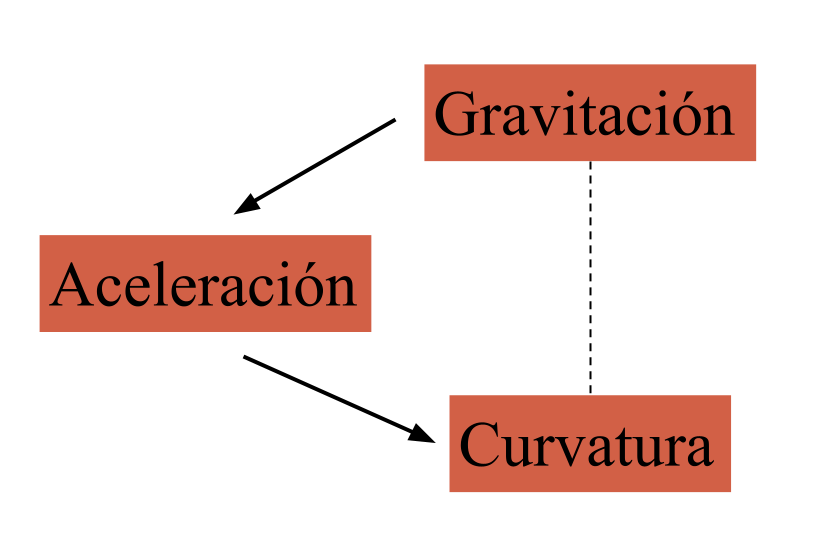
\includegraphics[width=0.7\textwidth]{Im/curvatura aceleracion.png}
    \label{fig:sen}
\end{figure}

\subsection*{\textbf{Gravedad y Aceleración}}

\begin{marginfigure}
\captionsetup{type=figure}
    \centering
    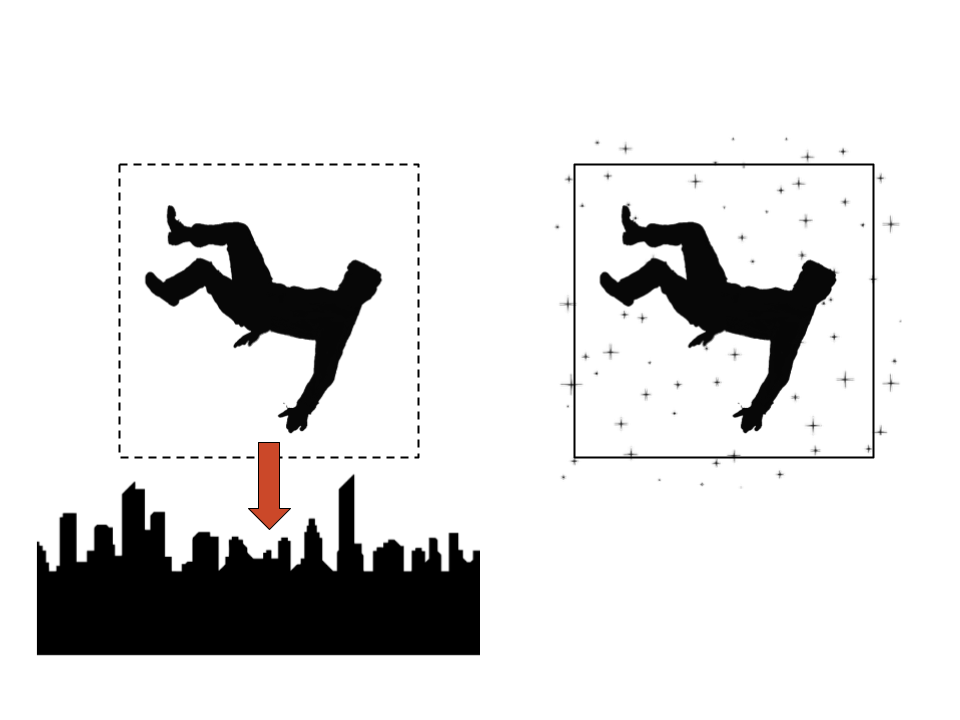
\includegraphics[width=1.3\textwidth]{Im/happiestthought.png}
    \caption{El pintor en caída libre no experimenta peso alguno, mientras cae siente lo mismo que si estuviera flotando libremente en el espacio.}
    \label{fig:sen}
\end{marginfigure}
En 1907, mientras trabajaba en una fábrica de patentes en Suiza, Einstein concibió lo que luego llamó su \textit{pensamiento más feliz}: al mirar por la ventana a un pintor en el exterior de un edificio, se imaginó qué sucedería si éste se cayera del andamio. Durante su caída, pensó, el pintor no experimentaría su propio peso (weightlessness). Es decir, en el sistema no-inercial solidario al pintor durante la caída desaparece la fuerza peso, podemos eliminar la interacción gravitatoria al considerar un sistema acelerado. Podemos decir que entonces \textbf{existe una analogía entre sistemas acelerados y sistemas bajo la influencia de campos gravitatorios}.

Esto es el llamado \textbf{Principio de Equivalencia}, sobre el cual hablaremos en detalle en la sección siguiente.

\subsection*{\textbf{Aceleración y Curvatura}}

Esta segunda relación es probablemente más difícil de comprender que la primera, principalmente porque aún no dimos una definición formal de curvatura en un espacio-tiempo. De momento, vamos a conformarnos con un ejemplo en el cual una medición realizada en un sistema inercial da un resultado distinto a una medición realizada en un sistema acelerado, anticipando que esta discrepancia en las mediciones guarda una estrecha relación con la definición de curvatura.

\begin{remarkbox}{Paradoja de Ehrenfest}
Consideremos un cilindro que rota uniformemente a velocidad $\omega$. Si realizamos una medición desde el sistema inercial del laboratorio, mediremos un radio $r$, y una circunferencia $c=2\pi r$.


Si, por otro lado, medimos desde un sistema solidario al cilindro, la \textbf{contracción de Lorentz} hará que las reglas del borde, que se mueven con velocidad tangencial a la circunferencia, se contraigan Tenemos que $c'>c=2\pi r$. Por otro lado, al medir el radio la velocidad es perpendicular a las reglas, y entonces $r'=r$.

Entonces, en nuestro sistema acelerado ya no vale que $c'=2\pi r'$. Esto ya nos puede dar una idea de que en un espacio curvado dejan de ser válidas las relaciones propias de la geometría euclidiana.

\end{remarkbox}
\begin{figure}
    \centering
    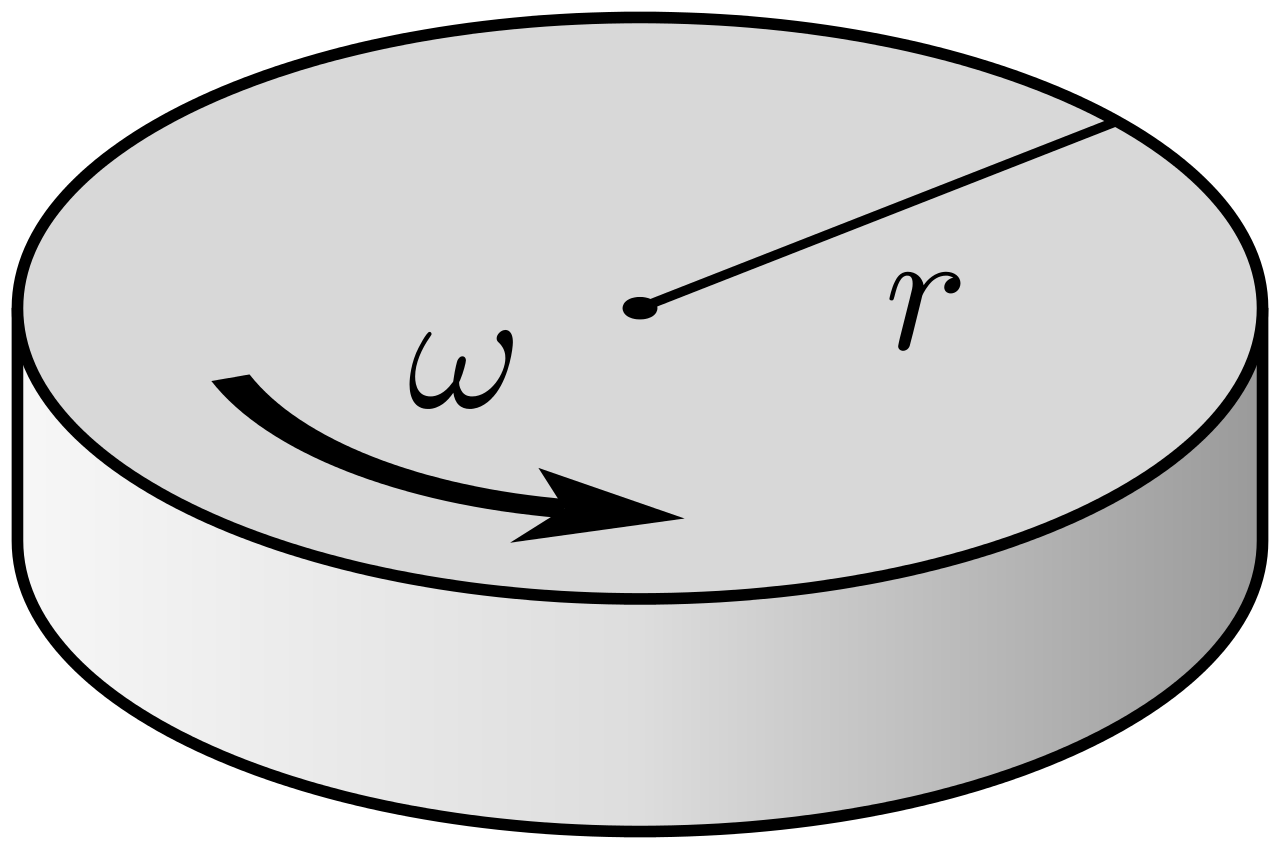
\includegraphics[width=0.315\textwidth]{Im/Spinning-disk.svg.png}
    \caption{Cilindro que rota con velocidad uniforme $\omega$.}
    \label{fig:sen}
\end{figure}

\begin{figure}
    \centering
    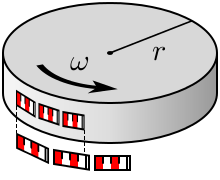
\includegraphics[width=0.3\textwidth]{Im/220px-Ehrenfest-paradox-disk.svg.png}
    \caption{Las reglas en el sistema laboratorio miden una circunferencia distinta a las del sistema no-inercial.}
    \label{fig:sen}
\end{figure}



¿Podemos concluir entonces que, mediante las dos relaciones establecidas, ya hemos vinculado interacción gravitatoria con curvatura del espacio-tiempo? Sí y no. Lo desarrollado es conceptualmente correcto, pero si queremos establecer una Teoría de la Relatividad General, donde Relatividad significa lo mismo que en Relatividad Especial, vamos a tener que \textbf{independizarnos de todo sistema de referencia}, incluidos los sistemas acelerados. Convencerse de esto ya es en sí mismo una tarea difícil (de hecho, le llevó a Einstein 7 años desprenderse de la idea de que las coordenadas nos dicen algo sobre el sistema estudiado\cite[][p.2-4]{wheeler}), pero además trae consigo la complicación de necesitar una formulación matemática que haga explícita esta independencia del sistema de coordenadas. Esto quiere decir que necesitamos una \textbf{formulación covariante} para las leyes, la cual se realiza a través de \textbf{tensores}\cite[][p.247]{landau2}.

Además, veremos que la equivalencia entre sistemas acelerados y gravitacionales es limitada: existen las denominadas \textbf{fuerzas de marea} (tidal forces), que nos imponen restricciones a la hora de construir nuestros sistemas. 

\begin{marginfigure}
\captionsetup{type=figure}
    \centering
    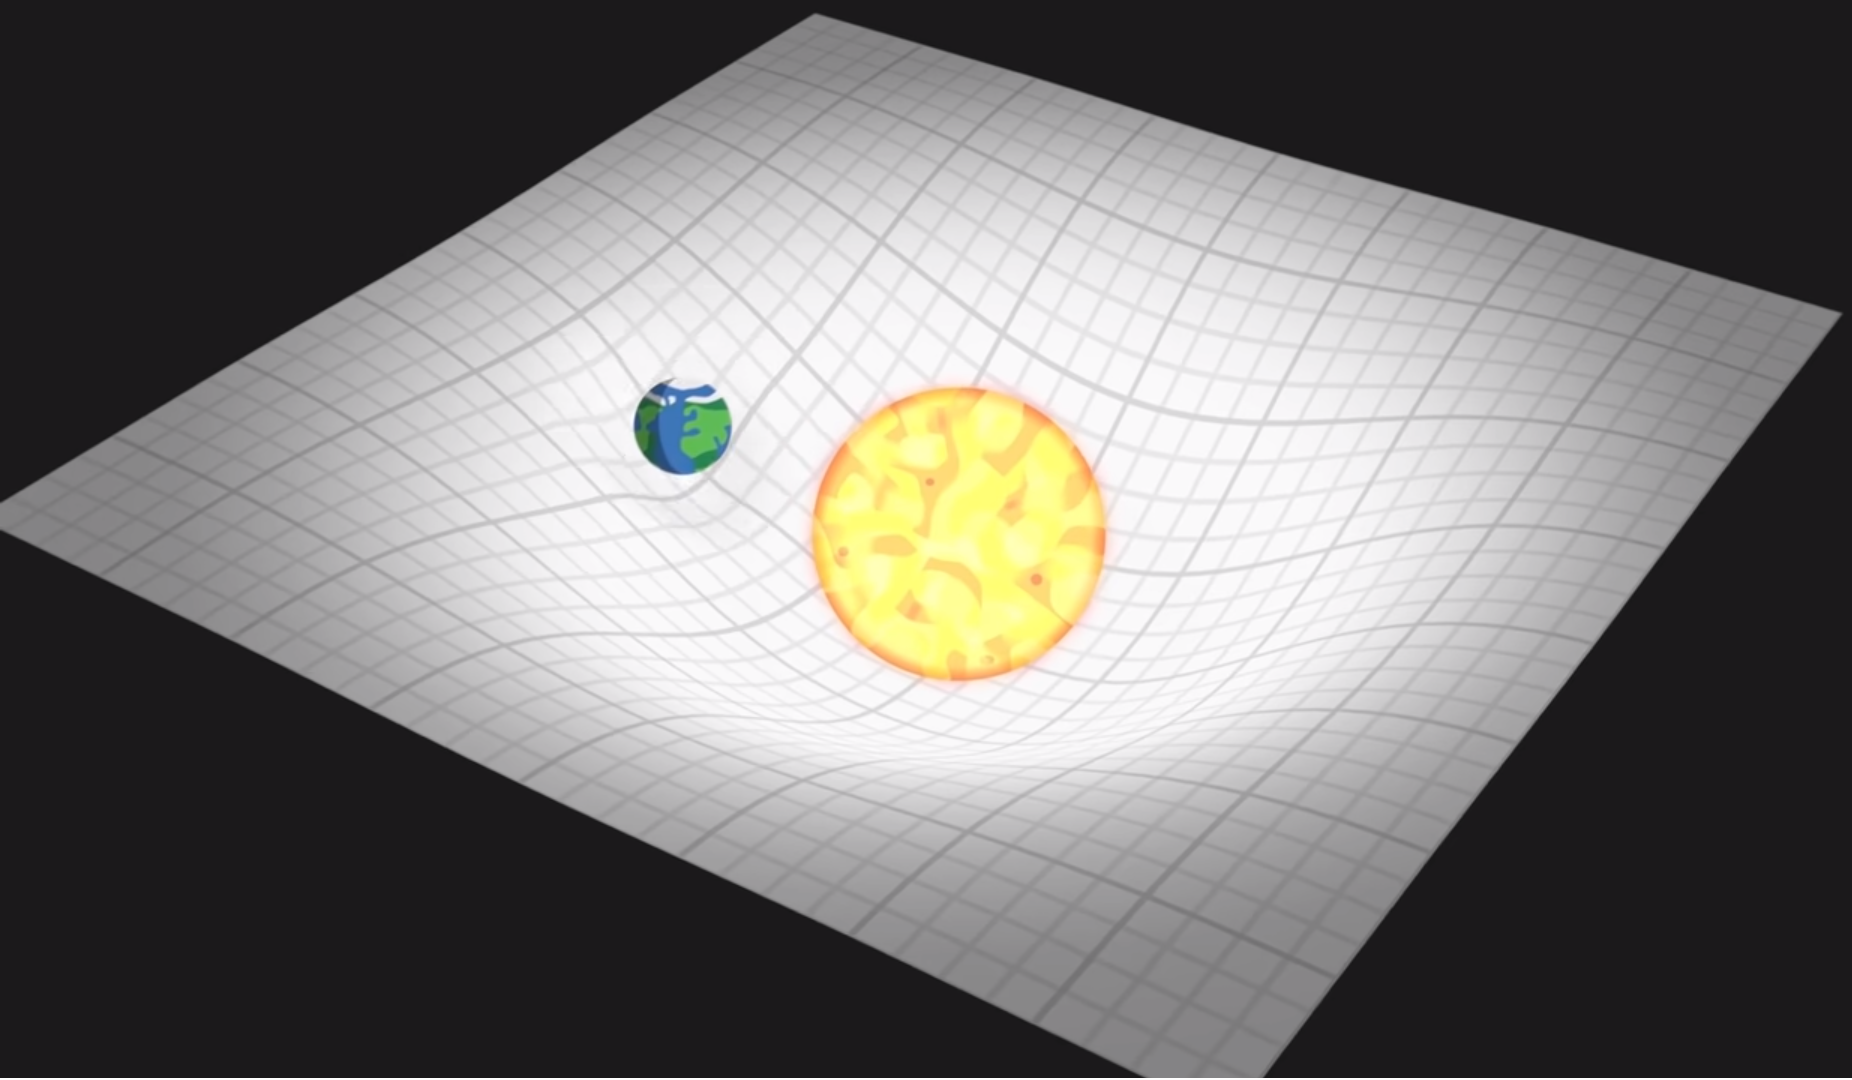
\includegraphics[width=1.3\textwidth]{Im/sistsolar.png}
    \caption{La masa del Sol curva el espacio-tiempo, y la Tierra se mueve en una geodésica a través de este espacio-tiempo curvado.}
    \label{fig:sen}
\end{marginfigure}

\newthought{Para concluir} con este breve resumen, mencionaremos la \textbf{hipótesis geodésica}, que en síntesis nos dice que \textbf{las partícula libres se mueven siguiendo una única trayectoria, denominada geodésica, que está definida por las características geométricas del espacio-tiempo.} Estas curvas pueden definirse como las líneas que \textbf{localmente más se asemejan a una recta}. Como estamos trabajando con un espacio-tiempo posiblemente curvo, las trayectorias muchas veces no se verán como líneas rectas, como es el caso de las órbitas de los planetas alrededor del Sol. 


\newpage

\section{\huge{Detalles del Principio de Equivalencia}}
\textcolor{myred}{\hrule width\textwidth}

\newthought{Volvamos a considerar} la Ley de Gravitación Universal, ahora con dos partículas de masas $M$ y $m_g$. Si incorporamos la Segunda Ley de Newton, tenemos que:

\begin{equation}
    F_g=G\frac{Mm_g}{r^2}=m_i a
\end{equation}

\begin{marginfigure}
\captionsetup{type=figure}
    \centering
    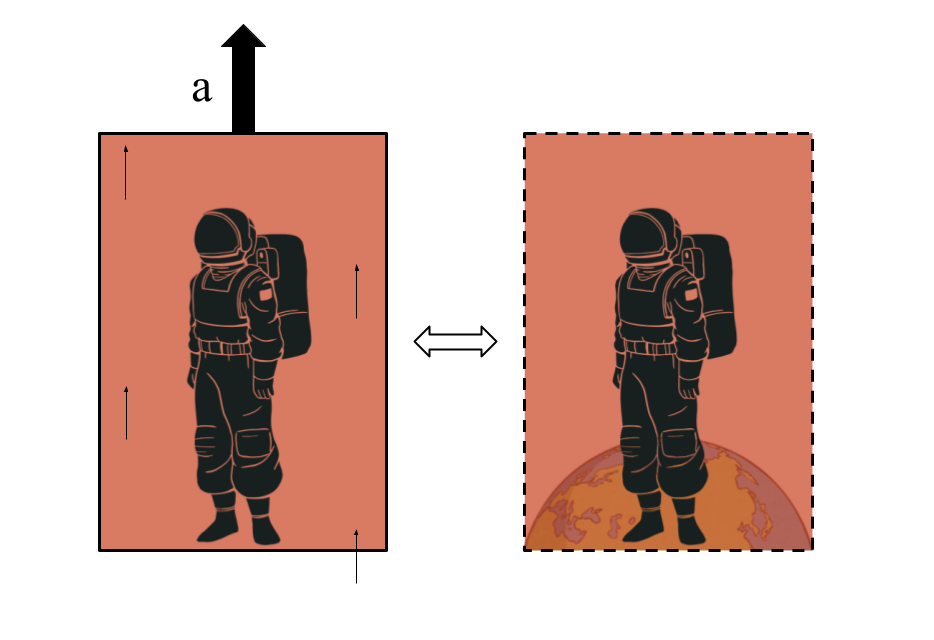
\includegraphics[width=1.3\textwidth]{Im/equiv.png}
    \caption{Principio de Equivalencia: lx cosmonauta o puede distinguir si está en un ascensor acelerándose hacia arriba en el espacio, o en un campo gravitatorio en reposo sobre la Tierra.}
    \label{fig:sen}
\end{marginfigure}

Donde $m_i$ es la \textbf{masa inercial} de la partícula, es decir, qué tanto 'se resiste' esta partícula a ser acelerada por una fuerza dada. Por otro lado, $m_g$ es la \textbf{masa gravitatoria}, la cual indica qué tan fuerte es la interacción de la partícula con un campo gravitatorio (de manera similar a la carga $Q$ en Electromagnetismo). Estos conceptos son \textbf{completamente diferentes}, y a priori no deberíamos esperar que estén relacionados entre sí\cite[][p.2]{moore}.

La experiencia demuestra que, en realidad, ambas masas sí son iguales, lo cual nos permite realizar la siguiente afirmación fundamental: \textbf{en un campo gravitacional, todos los cuerpos se mueven de la misma manera, independientemente de su masa.}

Es esta propiedad la que nos permite establecer la analogía entre campos gravitacionales y sistemas acelerados. Un ejemplo emblemático de esto es considerar un sistema alejado de cualquier campo gravitacional, que se acelera uniformemente a $9,8 m/s^2$. Unx observadorx en este sistema no tiene forma de reconocer si realmente se está acelerando, o si está 'en reposo' (es decir, en un sistema inercial) en la superficie de la Tierra.

\begin{figure}[h!]
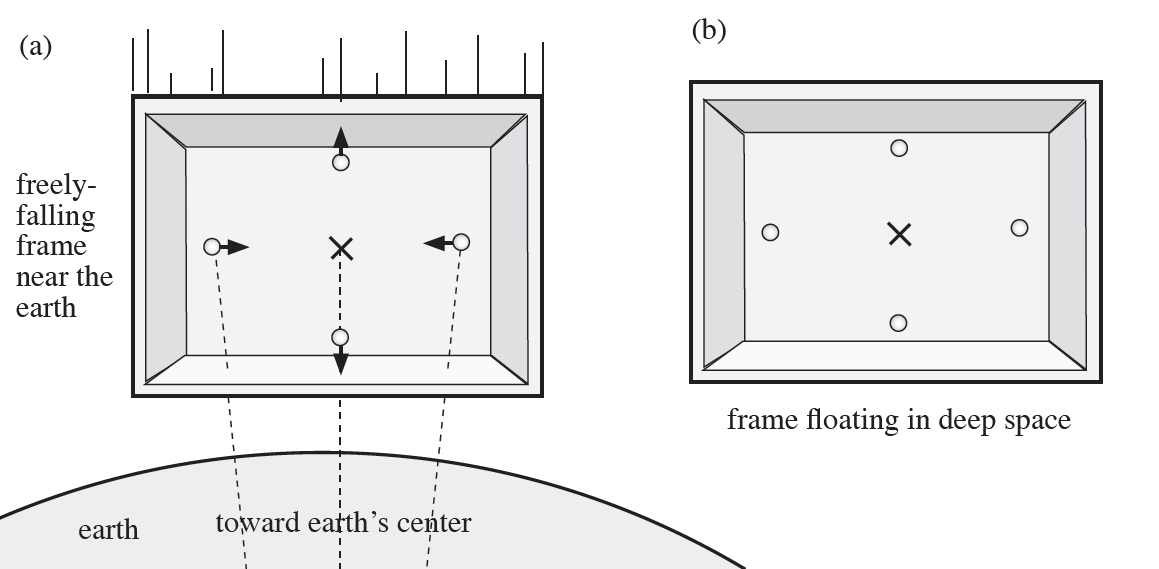
\includegraphics[width=\textwidth]{Im/tidal.png}
\caption{Si arrojáramos cuatro masas hacia la Tierra, la no-uniformidad del campo gravitatorio real haría que las masas de los costados se acerquen, y que las de arriba y abajo se alejen gradualmente. A esto se lo denomina \textbf{fuerzas de marea}, y no puede recrearse en un sistema que flota lejos de cualquier interacción gravitatoria.}
\label{fig:my_label}
\end{figure}

En realidad, lo enunciado anteriormente no es del todo cierto, por dos motivos:
\begin{itemize}
    \item Mientras que los campos gravitatorios \textit{siempre} tienden a cero al alejarse de la masa que los produce, los 'campos' asociados a sistemas acelerados no lo hacen. En el ejemplo recién mencionado, el 'campo' que mediría lx observadorx aceleradx sería igual en todos lados. En el ejemplo de la paradoja de Ehrenfest, la fuerza centrífuga que aparece en el sistema que rota se hace cada vez más grande a medida que nos alejamos del eje de rotación. 
    \item Los campos gravitatorios reales no son uniformes, por lo cual existen \textbf{fuerzas de marea} que tienden a comprimir o estirar cualquier cuerpo que se encuentre en ellos.
\end{itemize}

Es por esto que lo máximo que podemos hacer es, tomando un sistema no-inercial apropiado, eliminar el campo gravitatorio en una región lo suficientemente pequeña como para considerar al campo uniforme. El hecho de que los campos gravitatorios no puedan ser eliminados en su totalidad mediante la elección de un sistema de referencia, es una evidencia de la \textbf{realidad física} de los mismos.
\newpage
\section{\huge{Curvatura}}

\textcolor{myred}{\hrule width\textwidth}

\begin{flushright}
\textit{He visto a Lucy\\ Cuando entró a la habitación\\ El espacio se curvó}\\ \textbf{Gustavo Cerati}
\end{flushright}

\subsection*{\textbf{Coordenadas Curvilíneas}}
En esta sección, vamos a responder la ansiada pregunta: \textbf{¿qué es la curvatura?} Para ello, comencemos definiendo una \textbf{base de coordenadas} (Moore) o \textbf{coordenadas curvilíneas} (Landau). Sin importar qué tan complicado es nuestro espacio a considerar\footnote{Por simplicidad, de momento nos vamos a limitar a dos dimensiones $(u,w)$.}, siempre podemos definir\cite[][p.54]{moore}, en cada punto $\mathcal{P}$, un par de vectores $\mathbf{e}_u$ y $\mathbf{e}_w$ tales que:
\vspace{1cm}
\begin{fullwidth}
\begin{remarkbox}{Coordenadas Curvilíneas (en $2D$)}
\begin{itemize}
    \item $\mathbf{e}_u$ es tangente a la curva $w=cte$ y apunta en el sentido de $u$ creciente.
    \item $\mathbf{e}_w$ es tangente a la curva $u=cte$ y apunta en el sentido de $w$ creciente.
    \item Las longitudes de $\mathbf{e}_u$ y $\mathbf{e}_w$ son tales que el vector desplazamiento $d \mathbf{s}$ que va de $\mathcal{P}(u,w)$ a un punto infinitesimalmente cercano $(u+du,w+dw)$ puede escribirse como:
    $$d\mathbf{s}=du\mathbf{e}_u+dw\mathbf{e}_w=dx^{\mu}\mathbf{e}_{\mu}$$
\end{itemize}
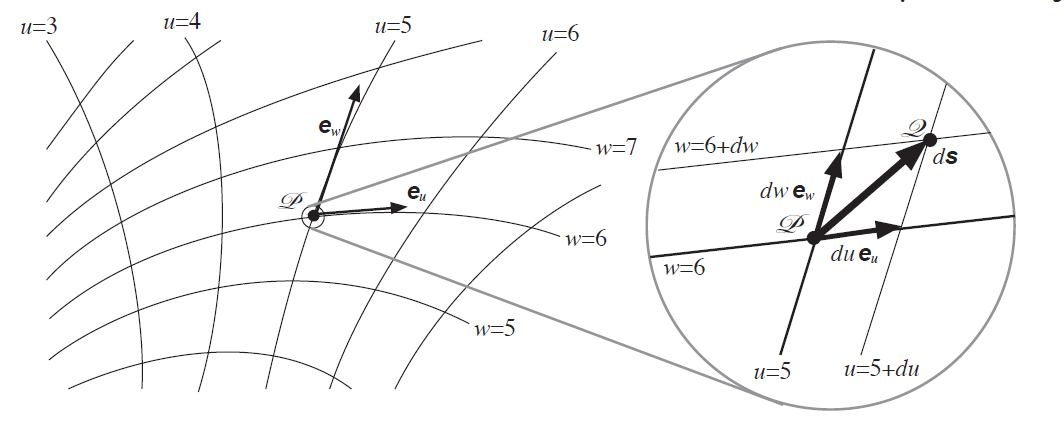
\includegraphics[width=1\textwidth]{Im/coord.png}
    \label{fig:sen}
\end{remarkbox}
\end{fullwidth}
Un sistema de coordenadas definido de esta manera puede resultar muy distinto a los versores cartesianos habituales, por los siguientes tres motivos: 

\begin{itemize}
    \item El producto escalar $\mathbf{e}_u \cdot \mathbf{e}_w$ puede ser \textbf{distinto de cero}.
    \item El módulo de $\mathbf{e}_u$ y $\mathbf{e}_w$ puede no ser igual a $1$.
    \item $\mathbf{e}_u$ y $\mathbf{e}_w$ pueden modificar sus módulos y/o direcciones a medida que nos movemos en el espacio.
\end{itemize}

\subsection*{\textbf{Tensor Métrico}}
\begin{marginfigure}
\captionsetup{type=figure}
    \centering
    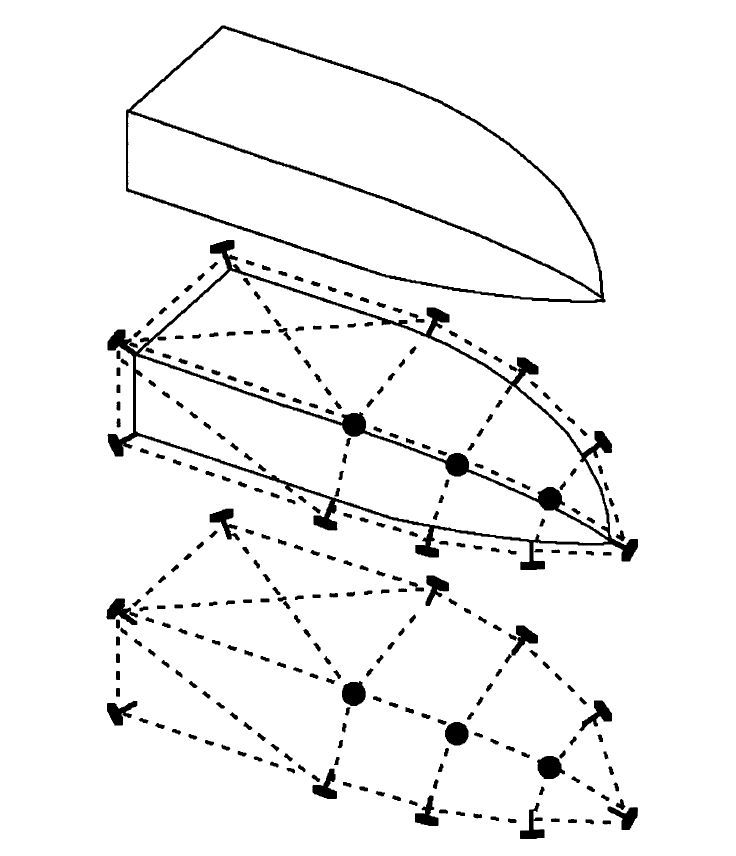
\includegraphics[width=1.3\textwidth]{Im/bote.png}
    \caption{Wheeler y Taylor explican que podemos estudiar la geometría de un espacio colocando 'clavos' (eventos) y anotando las distancias entre estos puntos.}
    \label{fig:sen}
\end{marginfigure}

Al igual que en Relatividad Especial, estamos interesadxs en estudiar \textbf{distancias entre eventos}, es decir, la separación espacial y temporal medida con reglas y relojes respecto a la cual todxs lxs observadorxs están de acuerdo: el \textbf{intervalo invariante}. En SR, ese intervalo se calculaba mediante:

\begin{equation}
    ds^2 = c^2 dt^2 -dx^2 -dy^2 - dz^2
\end{equation}

Un espacio con esta \textbf{métrica} se denomina espacio \textbf{de Minkowski} o \textbf{de Galileo}.

Pensemos ahora en un espacio con coordenadas curvilíneas como las que definimos antes. Aquí, tenemos que:

\begin{equation}
\begin{split}
    d s^2 &= d\mathbf{s} \cdot d\mathbf{s} = (du\mathbf{e}_u+dw\mathbf{e}_w)\cdot(du\mathbf{e}_u+dw\mathbf{e}_w)= \\
    &= du^2 \mathbf{e}_u \cdot \mathbf{e}_u + du\,dw \mathbf{e}_u \cdot \mathbf{e}_w + dw^2 \mathbf{e}_w \cdot \mathbf{e}_w = dx^\alpha dx^\beta \mathbf{e}_\alpha \cdot \mathbf{e}_\beta
\end{split}
\end{equation}

Esta ecuación especifica la relación entre la separación de puntos en una base curvilínea y el intervalo invariante (distancia física), y puede pensarse como una \textbf{generalización del Teorema de Pitágoras} para sistemas de coordenadas arbitrarias. A partir de aquí trabajaremos en el espacio-tiempo cuatridimensional habitual, es decir con $\mu=0,1,2,3$.

Esta ecuación nos invita a definir el \textbf{Tensor Métrico} de la siguiente manera:

\begin{remarkbox}{Tensor Métrico}
\begin{equation}
    g_{\mu\nu}\equiv \mathbf{e}_\mu \cdot \mathbf{e}_\nu
    \label{tensormetricobases}
\end{equation}
\end{remarkbox}

Podemos ver que esto es la generalización del tensor $\eta_{\mu\nu}$ propio de los espacios de Minkowski. Una métrica general tiene entonces la forma:

\begin{remarkbox}{Métrica}
\begin{equation}
    ds^2 = g_{\mu \nu}\,dx^\mu dx^\nu
\end{equation}
\end{remarkbox}

\subsection*{\textbf{Aceleración}}

Volvamos al ejemplo de un sistema no-inercial que rota uniformemente, y veamos cómo esto nos conduce a una métrica particular.

Si aplicamos las siguientes transformaciones, donde $\Omega$ es la velocidad angular de rotación, en la dirección del eje $z$:

$$x=x'\cos \Omega t-y'\sin \Omega t , \hspace{0.5cm} y=x'\sin \Omega t + y' \cos \Omega t, \hspace{0.5 cm}z=z'$$

Podemos llegar a un intervalo $ds$ con la siguiente forma\cite[][p.244]{landau2}:

\begin{equation}
\begin{split}
ds^2 = \left[c^2-\Omega^2(x'^2+y'^2) \right]dt^2-&dx'^2-dy'^2-dz'^2\\
&+2\Omega y' dx' dt-2\Omega x'dy'dt
\end{split}
\end{equation}

Sin importar cómo transformemos, \textbf{es imposible representar esta expresión como una suma de cuadrados de diferenciales de coordenadas} (es decir, no podemos llevar al tensor métrico a una forma diagonal). Además, vemos que el valor de las entradas de este tensor (es decir, de los coeficientes que acompañan a cada producto de diferenciales) varían al movernos en el espacio.

\subsection*{\textbf{Curvatura}}

\begin{flushright}
\textit{No se puede dar una clase de Relatividad General\\ sin agarrar una hoja de papel y doblarla.\\ \textbf{Fran Cassinese}}
\end{flushright}

\begin{marginfigure}
\captionsetup{type=figure}
    \centering
    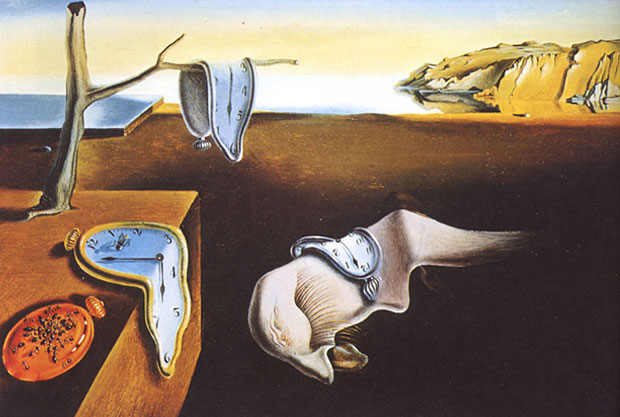
\includegraphics[width=1.3\textwidth]{Im/persistenceofmemory1931.jpg}
    \caption{\textit{La persistencia de la memoria}, de Salvador Dalí.}
    \label{fig:sen}
\end{marginfigure}

Apelando al Principio de Equivalencia, podemos decir que, si un sistema acelerado equivale a un espacio con una métrica particular que varía al hacer variar las coordenadas, entonces también \textbf{un campo gravitatorio es un cambio en la métrica del espacio-tiempo, determinado por las cantidades} $g_{\mu\nu}$. Ya estamos conectando la geometría del espacio-tiempo (su métrica) con fenómenos físicos (gravitación), independizándonos de las coordenadas (sistemas no-inerciales).

Aún nos falta definir un espacio-tiempo curvo, y para ello vamos a recordar la conclusión de la sección anterior: \textbf{un campo gravitatorio no puede eliminarse completamente tomando un sistema de referencia particular, sino que sólo podemos eliminarlo localmente}. Llevándolo al lenguaje del tensor métrico, \textbf{no existe transformación que lleve a $g_{\mu\nu}$ a una forma $\eta_{\mu\nu}$ (de Minkowski, o espacio-tiempo plano) para todo el espacio}. 
\begin{marginfigure}
\captionsetup{type=figure}
    \centering
    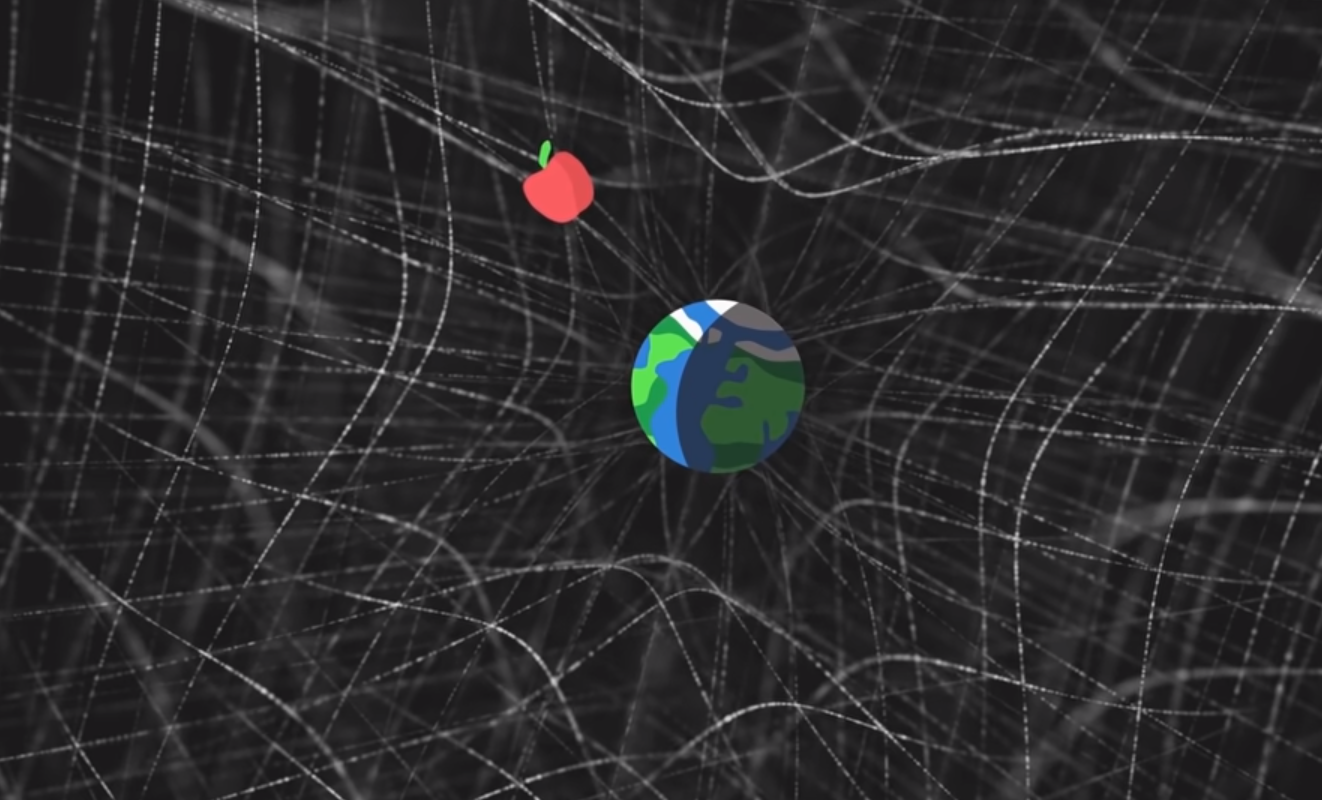
\includegraphics[width=1.3\textwidth]{Im/curve3d.png}
    \caption{Una manera de visualizar un espacio-tiempo curvo, que es conceptualmente más acertada, aunque no tan fácil de interpretar.}
    \label{fig:sen}
\end{marginfigure}

Y esta es justamente la definición de curvatura que vamos a utilizar\cite[][p.245]{landau2}:
\begin{remarkbox}{}
\textbf{Se dice que un espacio-tiempo está \textit{curvado} cuando su tensor métrico no puede reducirse al del espacio de Minkowski en todos lados}.
\end{remarkbox}
Como era de esperar, la curvatura es una \textbf{propiedad global} del espacio-tiempo, que puede aproximarse \textbf{localmente} por un espacio-tiempo plano (es decir, podemos eliminar la curvatura punto a punto), de la misma forma que la gravitación es una propiedad global del espacio-tiempo que puede eliminarse punto a punto eligiendo un sistema acelerado.

\subsection*{\textbf{Vectores Contravariantes y Covariantes}}

Ha llegado el momento de adentrarnos en el formalismo matemático propio de la Relatividad General. Como estamos interesadxs en cantidades que no dependan de los sistemas de coordenadas, vamos a definir muchos elementos \textit{según cómo transforman}. Si transformamos las coordenadas de las secciones anteriores, según la regla de la cadena se van a relacionar mediante:

\begin{equation}
    dx'^\mu=\frac{\partial x'^\mu}{\partial x^\nu}d x^\nu
\end{equation}

Si la base es una base curvilínea como las que vimos, las componentes $dx^\mu$ son en particular las componentes del desplazamiento $d\mathbf{s}$. Podemos entonces definir un \textbf{vector contravariante} $\mathbf{A}$, de modo tal que sus componentes se transformen como el desplazamiento $d\mathbf{S}$:

\begin{equation}
    A'^\mu=\frac{\partial x'^\mu}{\partial x^\nu}A^\nu
\end{equation}

Es posible ver que, si tomamos una función escalar de cuatro variables $\Phi$ y calculamos su gradiente $\partial_\mu \Phi$, este transformará de una forma distinta. En particular:

\begin{equation}
    \partial_\nu ' \Phi = \frac{\partial x^\mu}{\partial x'^\nu}\partial_{\nu}\Phi 
\end{equation}

Esto nos motiva a definir un \textbf{vector covariante}, cuyas componentes transforman como el gradiente $\partial_\mu \Phi$:

\begin{equation}
    B'_{\nu} = \frac{\partial x^\mu}{\partial x'^\nu}B_{\nu} 
\end{equation}

Combinando estos dos tipos de vectores, podemos construir tres tipos distintos de tensores:

\begin{remarkbox}{Tensores}
\begin{itemize}
    \item \textbf{Tensor contravariante} $A^{\mu\nu}$, cuyas componentes trasforman como los productos de las componentes de dos vectores contravariantes:
    
    $$A'^{\mu\nu}=\frac{\partial x'^\mu}{\partial x^\alpha}\frac{\partial x'^\nu}{\partial x^\beta}A^{\alpha \beta}$$
    
    \item \textbf{Tensor covariante} $A_{\mu\nu}$, cuyas componentes trasforman como los productos de las componentes de dos vectores covariantes:
    
    $$A'_{\mu\nu}=\frac{\partial x^\alpha}{\partial x'^\mu}\frac{\partial x^\beta}{\partial x'^\nu}A_{\alpha \beta}$$
    
    \item \textbf{Tensor mixto} $A^{\mu\nu}$, cuyas componentes trasforman como los productos de las componentes de dos un vector contravariante con uno covariante:
    
    $$A'^{\mu}_\nu=\frac{\partial x'^\mu}{\partial x^\alpha}\frac{\partial x^\beta}{\partial x'^\nu}A^{\alpha}_{\beta}$$
\end{itemize}
\end{remarkbox}

\newpage

\section{\huge{Cálculo de Curvatura}}
\textcolor{myred}{\hrule}

\newthought{Como introdujimos al hablar de curvatura}, un campo gravitatorio queda completamente descripto por la variación de un tensor métrico $g_{\mu\nu}$. Ahora bien, ¿cómo representamos dicha variación?. Un primer intento podría ser tomando el gradiente del tensor, de manera análoga a como tomamos el gradiente de un escalar para definir los covectores. Si tomamos un vector $A^\mu$ y calculamos su gradiente, conseguiremos una expresión de la forma $\partial_{\nu}A^{\mu}$. Si queremos transformarlo, tenemos que (utilizamos derivada del producto y definición de gradiente):

\begin{equation}
    \partial'_{\nu}A'^{\mu}=\frac{\partial x^{\beta}}{\partial x'^{\nu}}\frac{\partial^2 x'^\mu}{\partial x^\beta \partial x^\alpha}A^{\alpha}+\frac{\partial x^\beta}{\partial x'^\nu}\frac{\partial x'^{\mu}}{\partial x^{\alpha}}(\partial_\beta A^{\alpha})
\end{equation}

Si sólo tuviéramos el segundo término del lado derecho, entonces esta cantidad transformaría como un tensor, pero si los factores de transformación de coordenadas $\partial dx'^{\mu}/\partial d x^{\nu}$ no son constantes, entonces las derivadas segundas del primer término podrían no anularse. Esto quiere decir que las componentes del gradiente de un vector generalmente \textit{no} transforman como un tensor. Como hemos definido a los tensores según cómo transforman los vectores contravariantes y covariantes, lo mismo sucederá con el gradiente de un tensor, es decir que \textbf{el gradiente de un tensor no es un tensor}. Esto es un problema, ya que queremos construir una teoría con cantidades tensoriales, porque son independientes del sistema de referencia.

\subsection*{\textbf{Derivadas Primeras del Tensor Métrico}}

Para solucionar esto, pensemos en el caso más sencillo posible: un campo vectorial que es constante en todo el espacio. El gradiente 'verdadero' de este campo debería ser cero, y evidentemente en un sistema de coordenadas cartesiano, $\partial_{\mu}A^{\mu}=0$. Pero si tomamos un sistema de coordenadas curvilíneo, debemos tomar en cuenta las variaciones de los propios vectores de la base (los $\mathbf{e}_{\mu}$), que generalmente serán distintas de cero. 

\begin{marginfigure}
\captionsetup{type=figure}
    \centering
    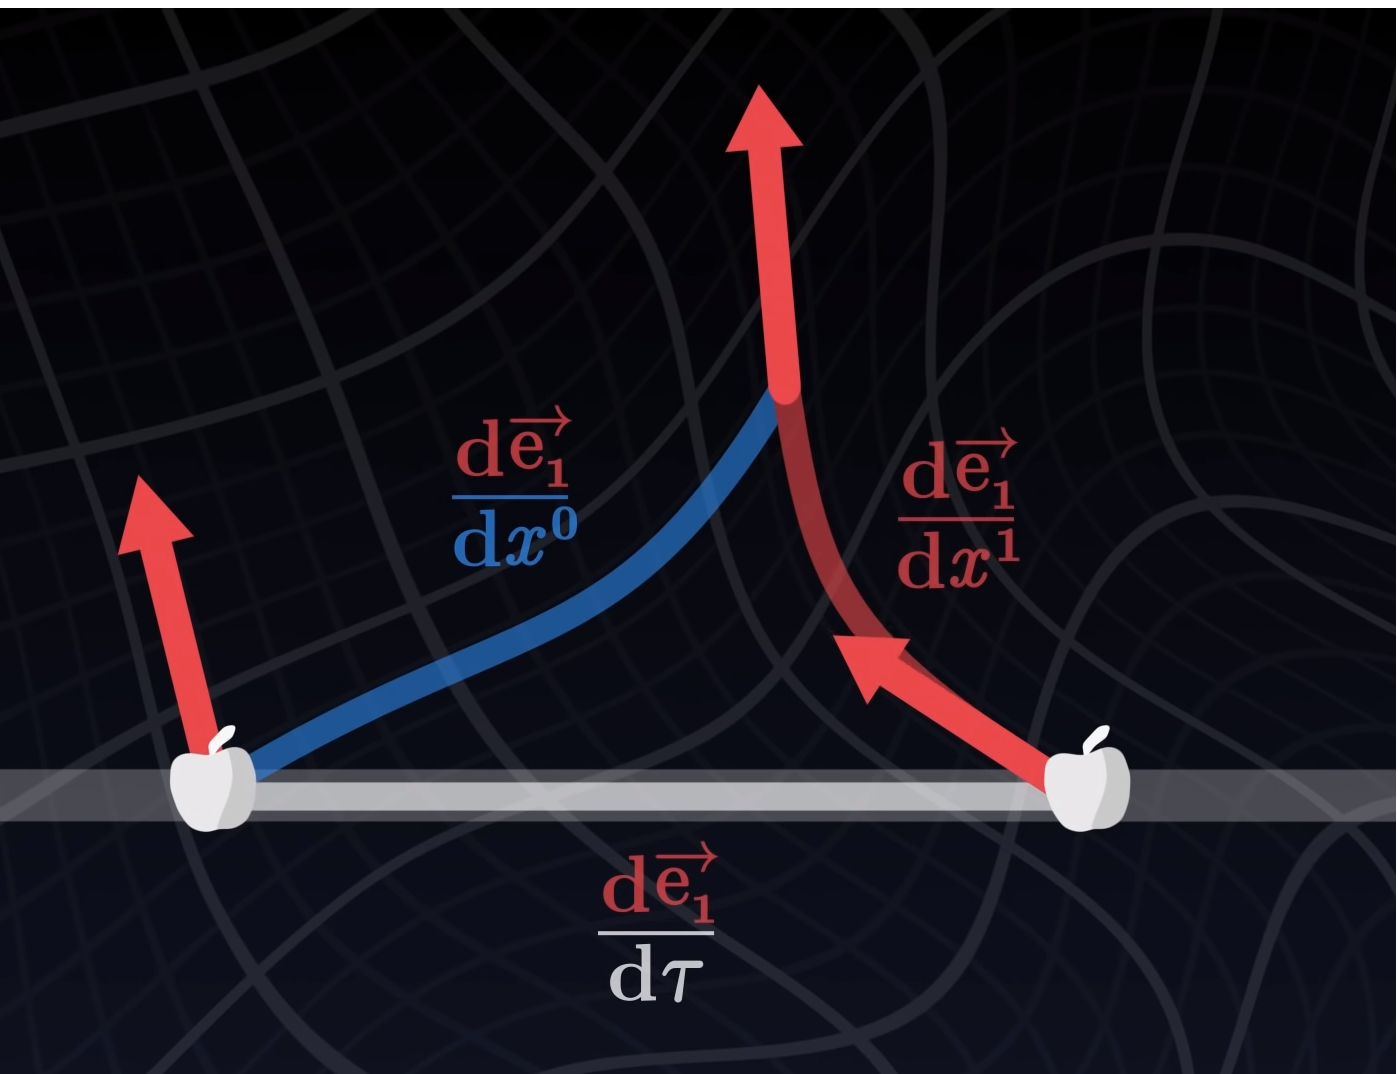
\includegraphics[width=1.3\textwidth]{Im/cambiocoord.png}
    \caption{Al estudiar la variación de un campo vectorial con coordenadas curvilíneas, debemos considerar el cambio del propio campo vectorial, y también el cambio de los vectores de la base.}
    \label{fig:sen}
\end{marginfigure}

Tomemos entonces un vector $\mathbf{A}(x^\mu)$, y veamos cómo varía al desplazarlo una cantidad infinitesimal $d\mathbf{s}$, de componentes $dx^\mu$:

\begin{equation}
d\mathbf{A}=d(A^\mu \mathbf{e}_{\mu})=\left(\frac{\partial A^{\mu}}{\partial x^{\sigma}}dx^\sigma \right)\mathbf{e}_{\mu}+A^\mu\frac{\partial \mathbf{e}_{\mu}}{\partial x^\alpha}dx^\alpha
\end{equation}

Vemos entonces que el primer término está relacionado a la variación del vector $\mathbf{A}$ al movernos en el espacio una cantidad $dx^{\mu}$, mientras que \textbf{el segundo término viene de la propia variación de los vectores de coordenadas curvilíneas}. Esto nos motiva a realizar dos definiciones nuevas:

\begin{remarkbox}{Símbolos de Christoffel}
Para un dado punto $\mathcal{P}$ en un espacio-tiempo con vectores de base $\mathbf{e}_{\mu}$, definimos los símbolos de Christoffel como los coeficientes $\Gamma^\nu_{\mu\alpha}$ que satisfacen:

\begin{equation}
    \frac{\partial \mathbf{e}_{\alpha}}{\partial x^{\mu}}\equiv \Gamma^\nu_{\mu\alpha} \mathbf{e}_{\nu}
\end{equation}

\end{remarkbox}

\begin{marginfigure}
\captionsetup{type=figure}
    \centering
    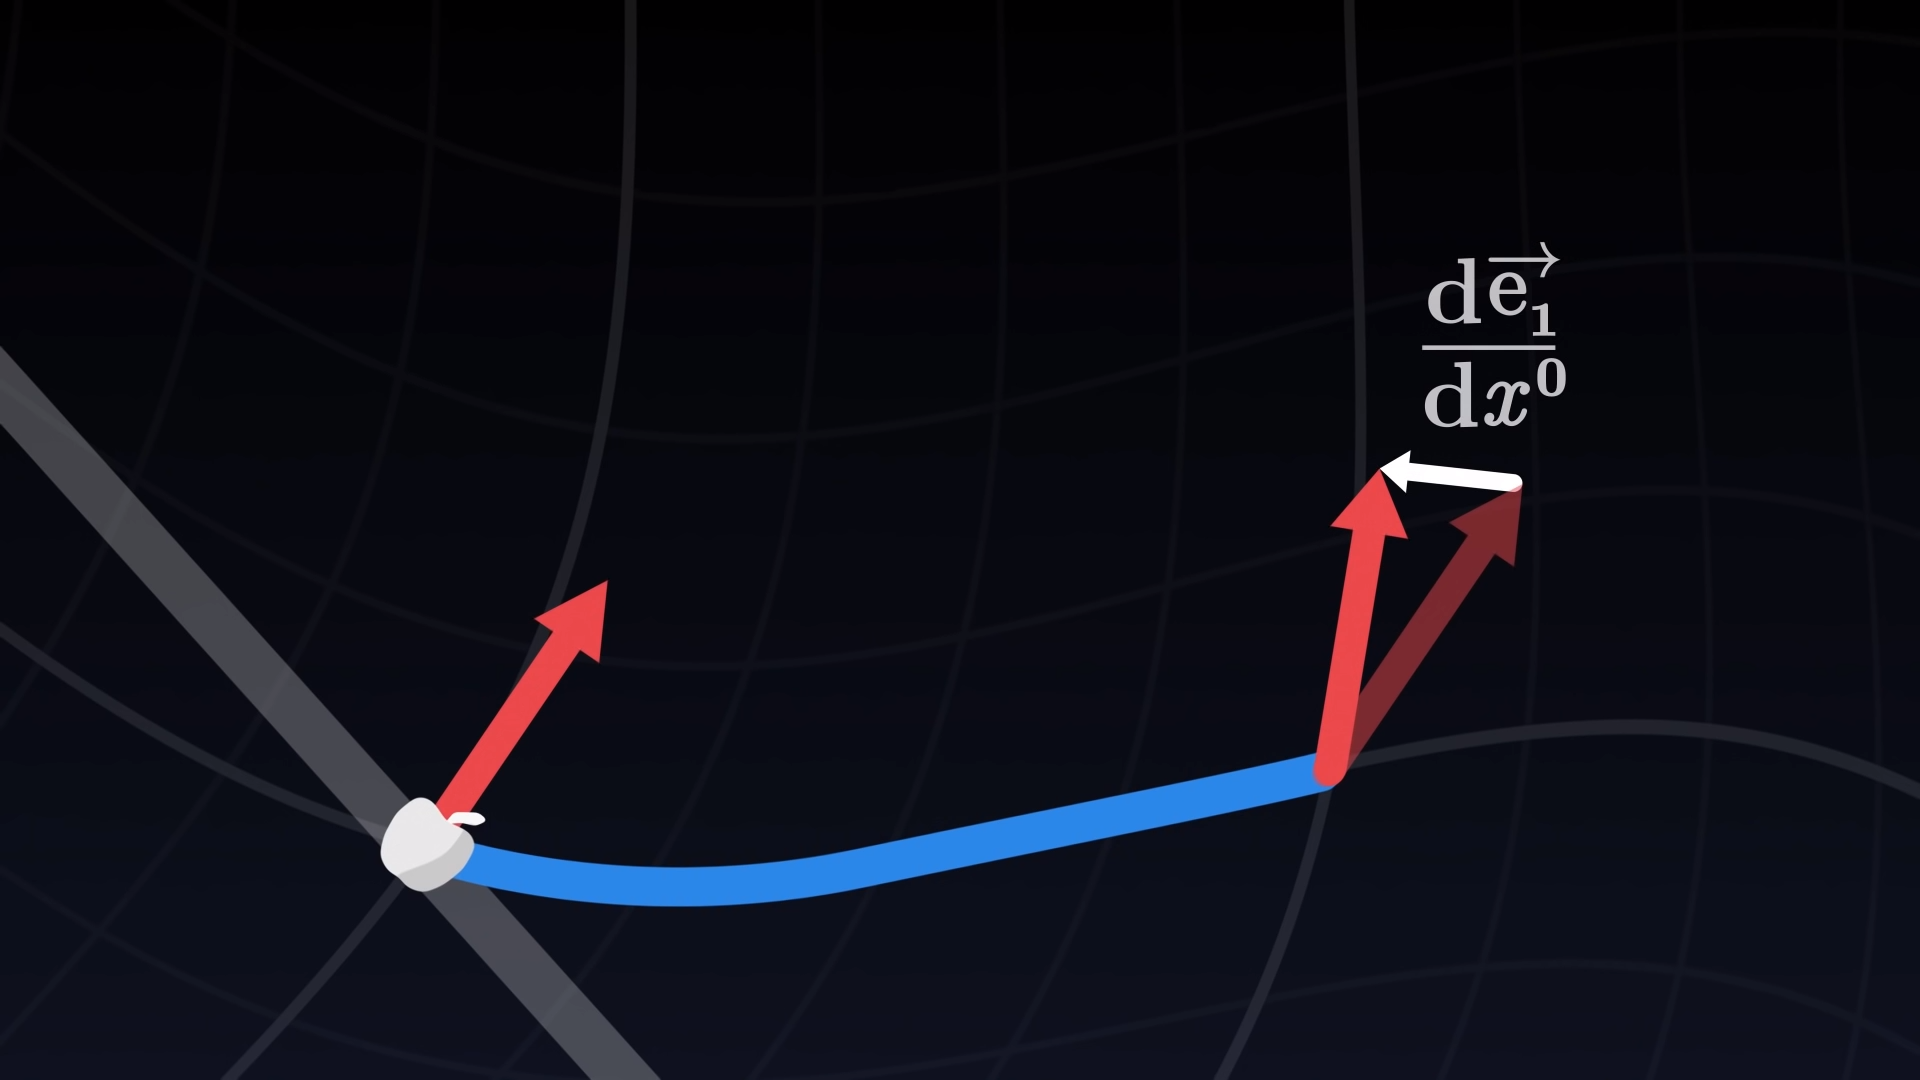
\includegraphics[width=1.3\textwidth]{Im/parallel.png}
    \caption{Transporte paralelo de un vector. Restando los vectores de cada punta obtenemos cómo cambia uno de los vectores de la base al variar la otra coordenada.}
    \label{fig:sen}
\end{marginfigure}

\begin{marginfigure}
\captionsetup{type=figure}
    \centering
    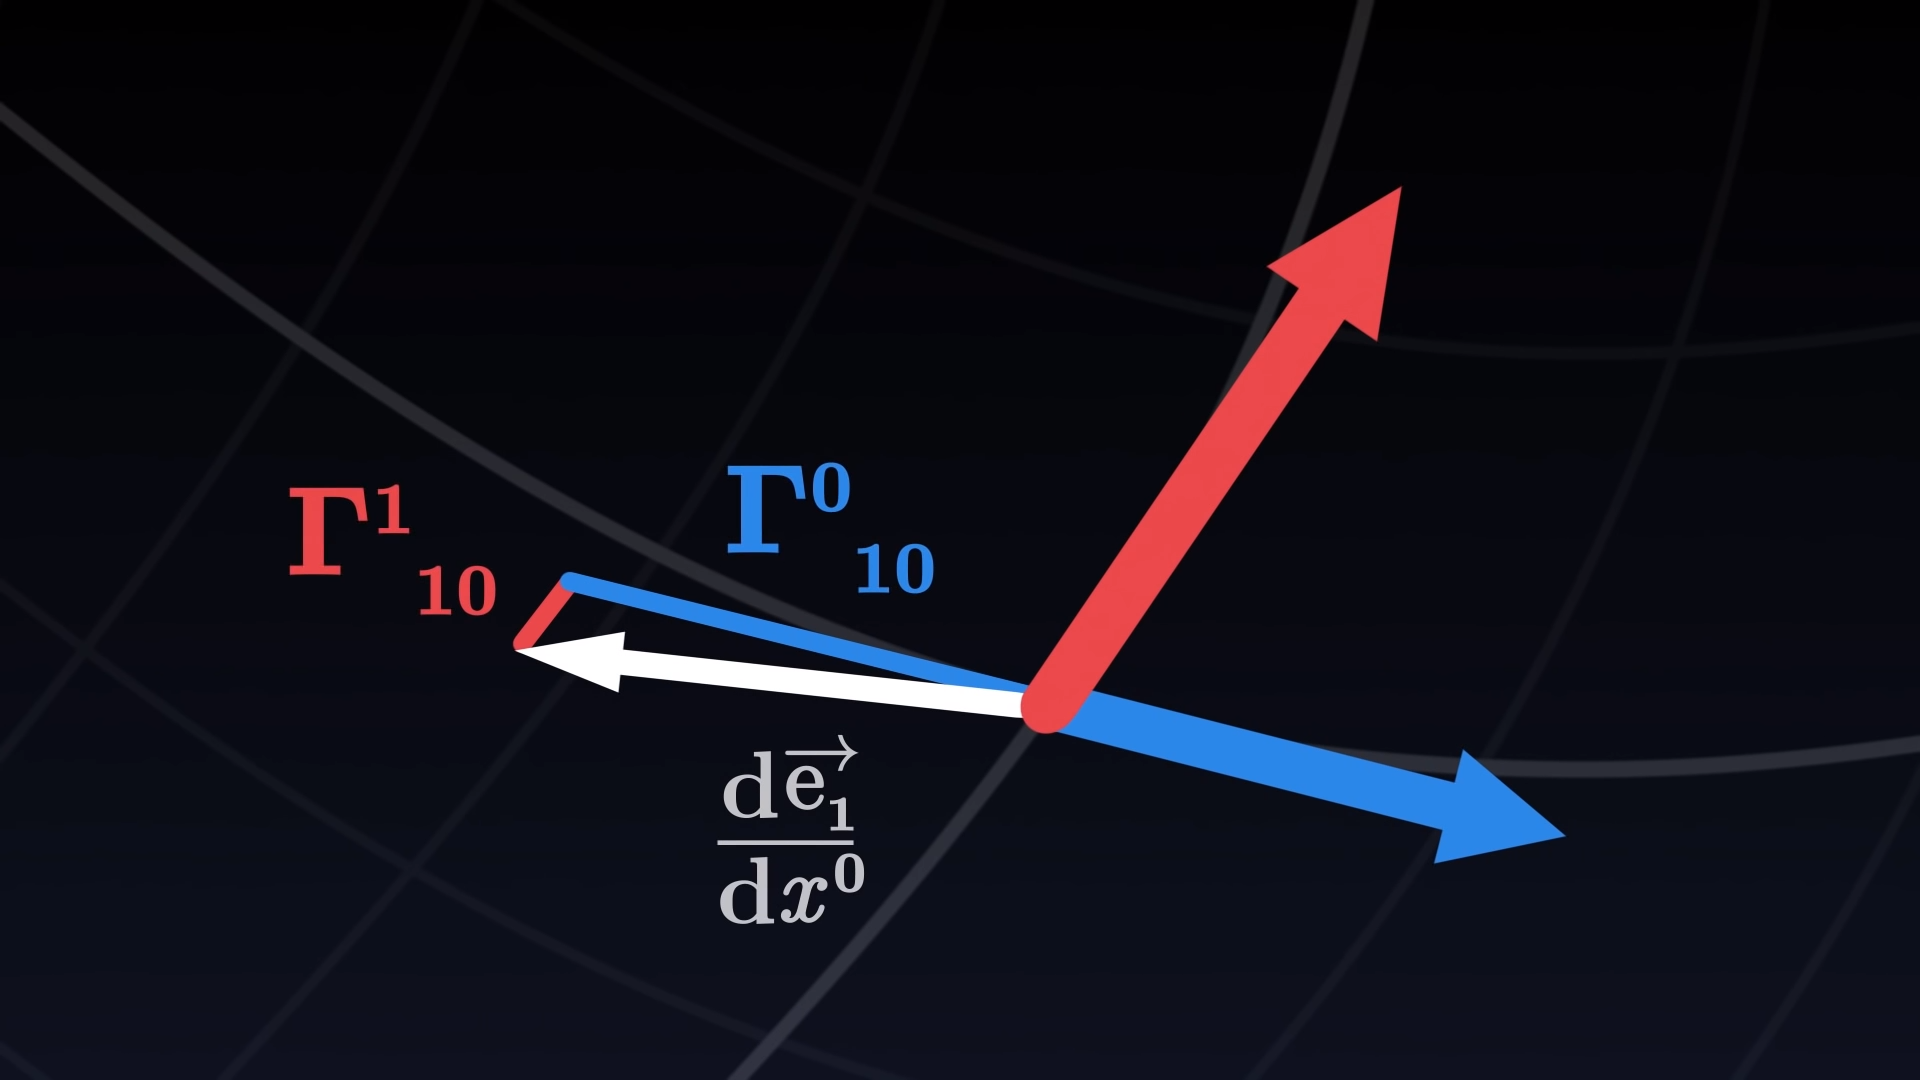
\includegraphics[width=1.3\textwidth]{Im/christoffel.png}
    \caption{Los símbolos de Christoffel representan cómo cambian los vectores de la base al desplazarnos en el mismo espacio, en las mismas coordenadas que estamos utilizando. Necesitamos tres índices, porque uno representa cuál es el vector $\mathbf{e}_{\mu}$ que estamos estudiando, otro indica cuál es la coordenada $x^{\nu}$ que hicimos variar, y el último cuál es la componente de la propia variación.}
    \label{fig:sen}
\end{marginfigure}

\begin{marginfigure}
\captionsetup{type=figure}
    \centering
    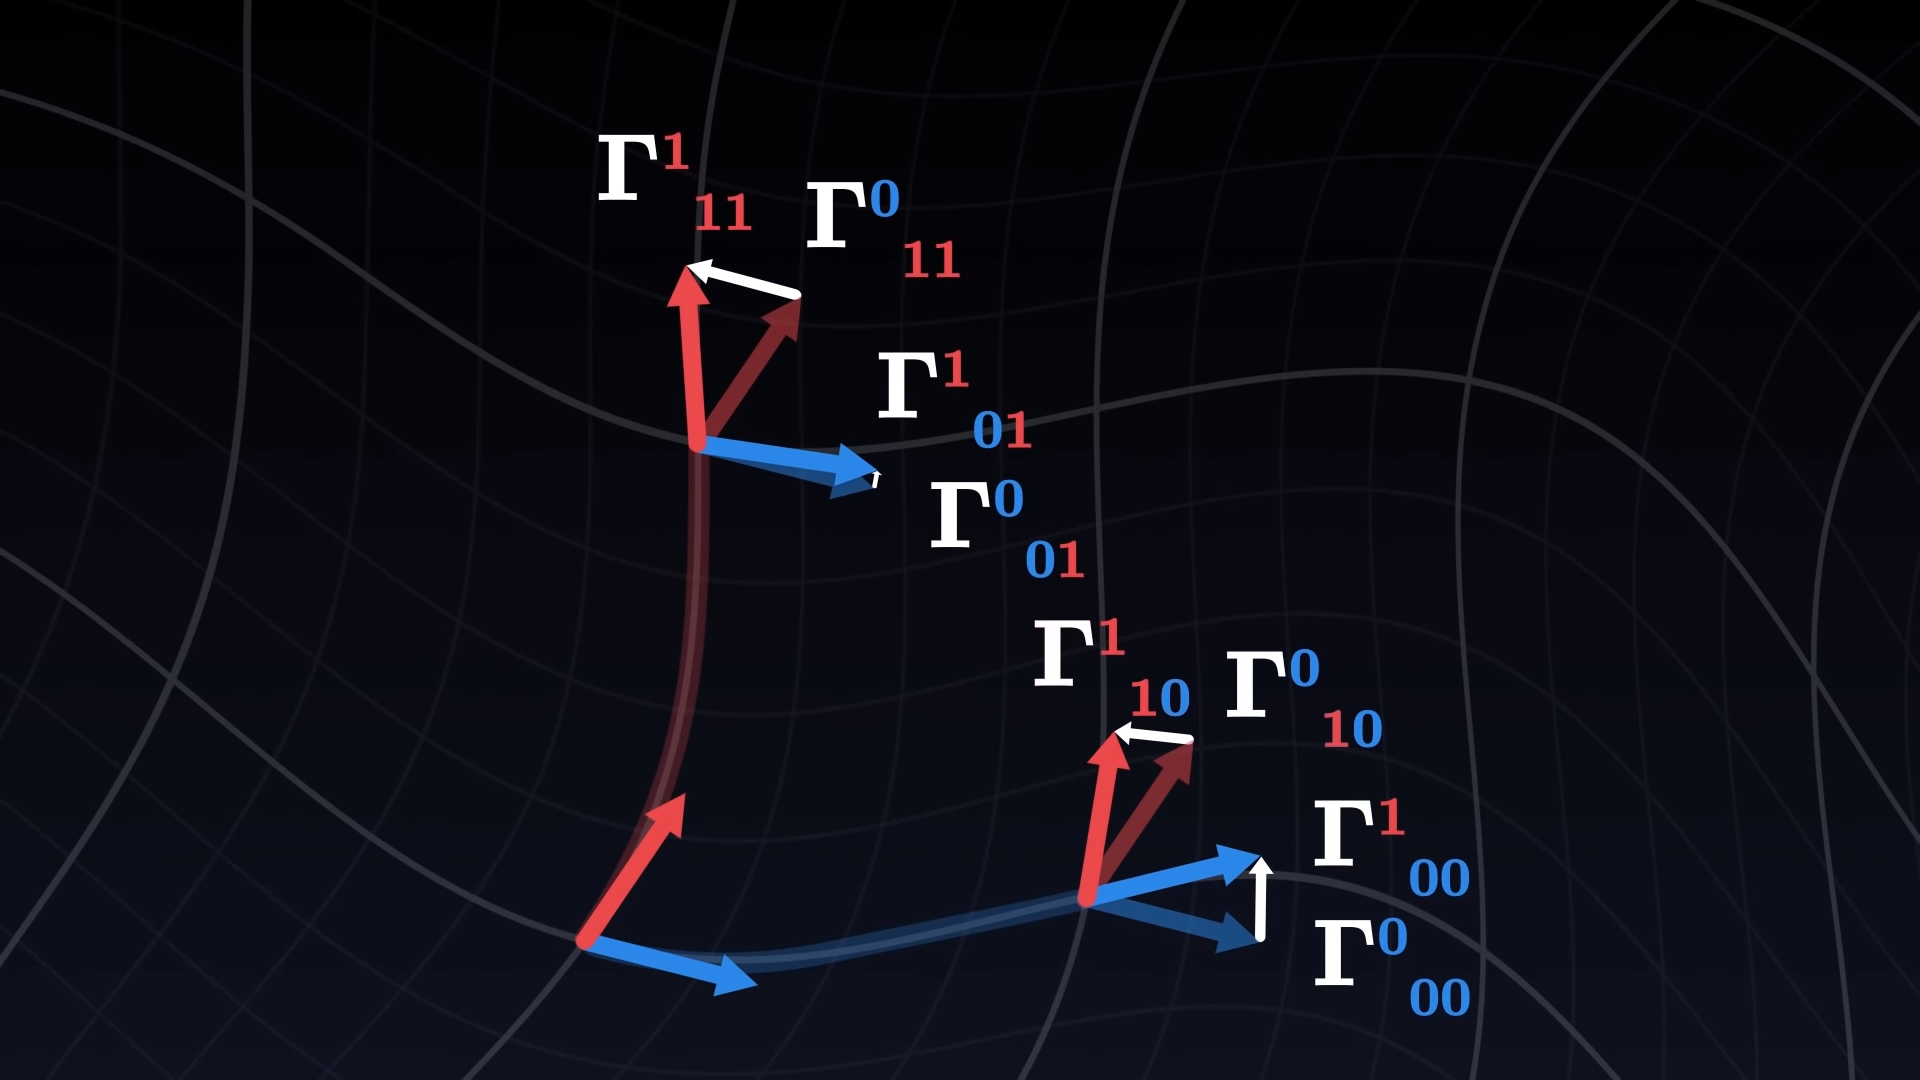
\includegraphics[width=1.3\textwidth]{Im/muchoscristoffel.png}
    \caption{En dos dimensiones, hay 8 símbolos de Christoffel para cada punto del espacio, de los cuales 6 son independientes.}
    \label{fig:sen}
\end{marginfigure}

Utilizando estos símbolos, podemos escribir a la ecuación para $d\mathbf{A}$ como:

\begin{equation}
    d\mathbf{A}= \left[\frac{\partial A^{\mu}}{\partial x^\alpha}+\Gamma^\mu_{\alpha \nu}A^{\nu}\right]\mathbf{e}_{\mu}dx^{\alpha}
\end{equation}

\begin{remarkbox}{Gradiente Absoluto (para un vector)}
        Definimos ahora el gradiente absoluto o derivada covariante de un campo vectorial $\mathbf{A}(x^{\alpha})$ según:
        
        \begin{equation}
            \nabla_\alpha A^{\mu}\equiv\frac{\partial A^{\mu}}{\partial x^\alpha}+\Gamma^\mu_{\alpha \nu}A^{\nu}
        \end{equation}
\end{remarkbox}


El gradiente absoluto es justamente la cantidad que estábamos buscando: un tensor que representa cómo varían los vectores al movernos en un espacio-tiempo curvo.

También podemos escribir, de manera análoga, el gradiente absoluto de un tensor:

\begin{remarkbox}{Gradiente Absoluto (para un tensor)}
\begin{equation}
\nabla_\gamma T^{\alpha\beta} = \partial_\gamma T^{\alpha\beta} + \Gamma^\alpha_{\mu\gamma}T^{\mu\beta} + \Gamma^\beta_{\mu\gamma}T^{\alpha\mu}
\end{equation}
\end{remarkbox}

Por otro lado, podemos interpretar los símbolos de Christoffel como sigue: realizamos el \textbf{transporte paralelo} de un vector, que significa desplazar un vector de forma paralela a sí misma, de modo tal que en coordenadas cartesianas conseguiríamos el mismo vector. Como estamos en coordenadas curvilíneas, los vectores aquí sí varían.


Ahora tomamos la variación del vector al realizar el transporte paralelo, y lo descomponemos en las componentes según los vectores de la base en ese mismo punto. Estas componentes son los símbolos de Christoffel.

Los símbolos de Christoffel son \textbf{simétricos} en sus dos índices inferiores, lo cual reduce la cantidad de símbolos independientes de 64 a 40. 

Además, si tomamos la definición de los símbolos de Christoffel y hacemos el producto escalar con algún otro vector de la base, podemos establecer una relación entre los $\Gamma^{\alpha}_{\mu \nu}$ y el tensor métrico. Esta es:

\begin{remarkbox}{}
\begin{equation}
    \Gamma^{\alpha}_{\mu \nu}=\frac{1}{2}g^{\alpha\sigma}\left[\partial_{\mu}g_{\nu\sigma}+\partial_{\nu}g_{\sigma \mu}-\partial_{\sigma}g_{\mu\nu}\right]
    \label{simboloChristoffel}
\end{equation}
\end{remarkbox}

Donde $g^{\alpha\sigma}$ es la \textbf{inversa} del tensor métrico (en el sentido matricial de inversa), es decir que $g^{\alpha\sigma}g_{\sigma\beta}=\delta^{\alpha}_\beta$.

\vspace{0.5cm}

Perfecto, ya tenemos una cantidad asociada a la variación del tensor métrico, ¿estamos en condiciones de expresar la curvatura del espacio-tiempo matemáticamente? \textbf{No}. Si hacemos memoria, localmente podemos aproximarnos a todo punto mediante un sistema cartesiano, cuya métrica es $\eta_{\mu\nu}$. Es decir que, además de reducir la métrica a la del espacio plano, también tenemos que, en ese punto, $\partial_\alpha g_{\mu\nu}=0$. No sólo eso, sino que además, en estos sistemas (llamados \textbf{localmente inerciales}), el gradiente absoluto se reduce al gradiente ordinario (por ser sistemas cartesianos), y entonces:

\begin{equation}
    \nabla_{\alpha}g_{\mu\nu}=\partial_\alpha g_{\mu\nu}=0
\end{equation}

Notemos que esta última es una ecuación tensorial, es decir que es independiente del sistema de coordenadas, de donde concluimos que \textbf{el gradiente absoluto del tensor métrico es nulo en todo sistema de referencia}.

\subsection*{\textbf{Derivadas Segundas del Tensor Métrico}}

Resulta que la verdadera información sobre la curvatura de un espacio-tiempo yace en las derivadas de segundo orden. Mediante un análisis de \textbf{desviaciones geodésicas}\cite[][p.211]{moore} (que aquí se ha omitido), podemos construir el llamado \textbf{Tensor de Riemann}, del cual daremos la definición y sus características fundamentales.

\begin{remarkbox}{Tensor de Riemann}
        Definimos al tensor de Riemann $R^\alpha_{\mu \nu \sigma}$ según:
        \begin{equation}
            R^\alpha_{\mu \nu \sigma}\equiv\partial_{\nu}\Gamma^{\alpha}_{\mu \nu}-\partial_{\sigma}\Gamma^{\alpha}_{\mu\sigma}+\Gamma^{\alpha}_{\mu\gamma}\Gamma^{\gamma}_{\mu\sigma}-\Gamma^{\alpha}_{\sigma\gamma}\Gamma^{\gamma}_{\mu\nu}
            \label{riemann}
        \end{equation}
        
        Sobre él podemos decir:
        \begin{itemize}
            \item Tiene 256 entradas, pero debido a las muchas simetrías del mismo, sólo 20 son independientes.
            \item Es \textbf{nulo para espacios planos}, y \textbf{no nulo para espacios curvados}, lo que lo hace la herramienta ideal para analizar la curvatura del espacio estudiado.
        \end{itemize}
\end{remarkbox}

Vamos a definir también otras cantidades que nos resultarán útiles a la hora de armar las Ecuaciones de Campo de Einstein.

\begin{remarkbox}{Tensor de Ricci}
        Definimos al tensor de Ricci $R_{\beta\nu}$ como la \textbf{contracción} del tensor de Riemann sobre su primera y tercera componente:
        \begin{equation}
            R_{\beta\nu} \equiv R^\alpha_{\beta \alpha \nu} \equiv g^{\alpha \mu} R_{\alpha\beta\mu\nu}
            \label{ricci}
        \end{equation}
        
        Este tensor es simétrico, y tiene 10 entradas independientes.
\end{remarkbox}

\begin{remarkbox}{Escalar de Curvatura}
        A su vez, definimos el escalar de Ricci o escalar de curvatura $R$ como la contracción del tensor de Ricci:
        \begin{equation}
            R \equiv g^{\beta\mu}R_{\beta\mu}\equiv g^{\beta\mu}g^{\alpha \mu} R_{\alpha\beta\mu\nu}
        \end{equation}
        
        Es interesante porque esta cantidad es un \textbf{escalar relativista}, es decir su valor no depende de la elección de coordenadas.
        
        Si $R_{\beta\nu} \neq 0$ o $R\neq 0$, ya podemos asegurar que el espacio está curvado, mientras que el recíproco no siempre es válido.
\end{remarkbox}


%Review of GR 
%\chapter{\textcolor{myred}{Ecuaciones de Campo de Einstein}}

\newthought{La validez} de la teoría gravitacional de Newton es indiscutible. Sobre las bases de esta teoría podemos determinar el movimiento de planetas, satélites, naves espaciales y hasta fuimos capaces de predecir la existencia de planetas\footnote{Urbain Le Verrier en 1846 predijo la existencia Neptuno debido a unas inconsistencias observadas en la órbita de Urano, usando las leyes de Kepler y Newton. Años más tarde, tal vez sugestionado por su descubrimiento anterior, Le Verrier interpretó que la anomalía en la órbita de Mercurio era debido a un planeta no descubierto que llamo Vulcano. Esto se vio reforzado por un astrónomo que creyó haberlo visto en su telescopio cuando en realidad solo vió una mancha en el lente.}.
De esta manera, a pesar que la teoría gravitacional de Newton entra en conflicto con el principio de equivalencia y las leyes de conservación del momento, la validez esencial de la teoría fue establecida y aceptada durante muchos años. Antes que pensar que la teoría está mal o es incorrecta, porque además, qué está bien o qué mal, está sujeto al contexto y a los conocimientos presentes en un determinado momento de la historia. La verdad no es un absoluto, si no, un acuerdo o consenso entre las personas y esto conlleva a muchas limitaciones. En otras palabras la teoría de Newton es un modelo que sirve para describir gran cantidad de fenómenos de la naturaleza y de forma perfectamente válida, no obstante es plausible que la dicha teoría esté incompleta y necesite ser más desarrollada. En particular, debe ser reformulada de manera tal que cumpla con el principio de equivalencia y satisfaga las leyes de conservación del momento.

\newthought{El objetivo de este capítulo} es construir las ecuaciones tensoriales que describan de una vez por todas los campos gravitatorios. Para ello, comencemos pensando en la \textbf{Ley de Gauss} para el Electromagnetismo, que conecta el campo eléctrico $\mathbf{E}$ con la densidad de carga $\rho$:
    $$\nabla \cdot \mathbf{E}= 4\pi k \rho$$
Cuando desarrolló su Teoría de Gravitación Universal, Newton no contaba con el concepto de campo, pero hoy en día podemos construir un análogo a la Ley de Gauss, para el campo gravitatorio $\mathbf{g}=-\nabla \Phi$ (donde $\Phi$ es el \textbf{potencial gravitatorio}), y una densidad de masa $\rho$:
    $$-\nabla \cdot \mathbf{g}= 4\pi G \rho \hspace{0.5cm}\Longrightarrow\hspace{0.5cm} \nabla^2\Phi=4\pi G\rho$$
Esta ecuación ya tiene una característica favorable: es una \textbf{ecuación de campo local}, es decir que relaciona la derivada del campo con su fuente \textit{en el mismo punto}. Esto nos ahorra el problema de señales instantáneas que presentamos al principio, y también nos permite considerar sistemas localmente inerciales, algo a lo que ya deberíamos estar acostumbradxs. 

Nuestro objetivo será entonces generalizar esta última ecuación. En base a lo que hemos estudiado, podemos anticipar que tendrá esta forma:

\begin{figure}[h!]
    \centering
    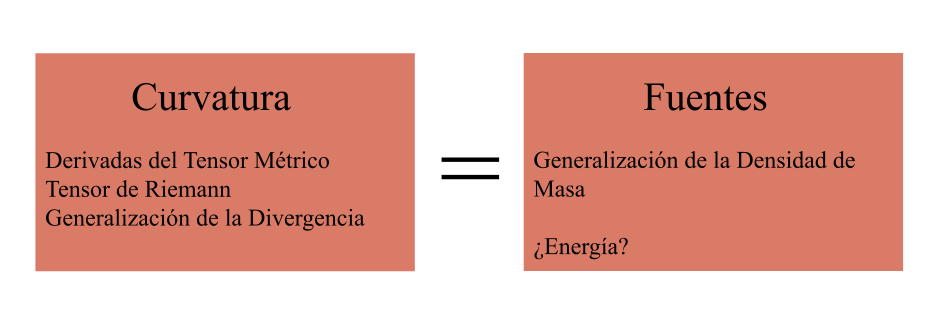
\includegraphics[width=0.95\textwidth]{Im/eceinstein.png}
    \label{fig:sen}
\end{figure}

\newpage
\section{\huge{Tensor de Estrés-Energía}}
\textcolor{myred}{\hrule}
\begin{flushright}
\textit{Anxiety is a scalar,\\fear is a vector,\\stress is a tensor.\\\textbf{Elon Musk} (War Criminal)}
\end{flushright}
El objetivo de esta sección es generalizar la densidad de masa escalar $\rho$ a una magnitud tensorial. Es decir, vamos a trabajar con el lado derecho de la ecuación, las \textit{fuentes}.

\vspace{0.5cm}

Primero podríamos preguntarnos, ¿en la ecuación newtoniana, la densidad $\rho$ representa la masa de un objeto, o es en realidad su \textbf{energía relativista}? En el límite newtoniano, estas dos magnitudes son equivalentes. Se puede demostrar (algo que no haremos aquí), que si la fuente del campo fuera la masa, podríamos crear energía \textit{de la nada}, mientras que 
si consideramos la energía como fuente de la gravedad, esto no sucede.

\vspace{0.25cm}

Lo siguiente sería pensar si $\rho$ pudiera ser una de las entradas de un tensor, de la misma manera que la densidad de carga $\rho$ resultó ser la componente temporal $J^{0}$ de el cuadrivector densidad de corriente $\mathbf{J}$. A este último resultado (propio de la Relatividad Especial), se llega mediante la \textbf{conservación de la carga}, así que podríamos esperar llegar a algo similar aquí apelando a la \textbf{conservación de la energía}.

La construcción de este tensor no es nada trivial, y puede visualizarse mejor mediante ejemplos: la energía-momento del \textbf{polvo} (partícula que se mueven estando en reposo unas respecto de las otras), o la energía-momento de un \textbf{fluido perfecto} (un conjunto de partículas que se mueven aleatoriamente pero no interactúan entre sí, por ejemplo un gas ideal). Vamos a pasar por alto estos ejemplos y caer directamente en el tensor, explicando sus componentes y sus propiedades:
\begin{remarkbox}{Tensor de Estrés-Energía o Energía-Momento}
    \centering
    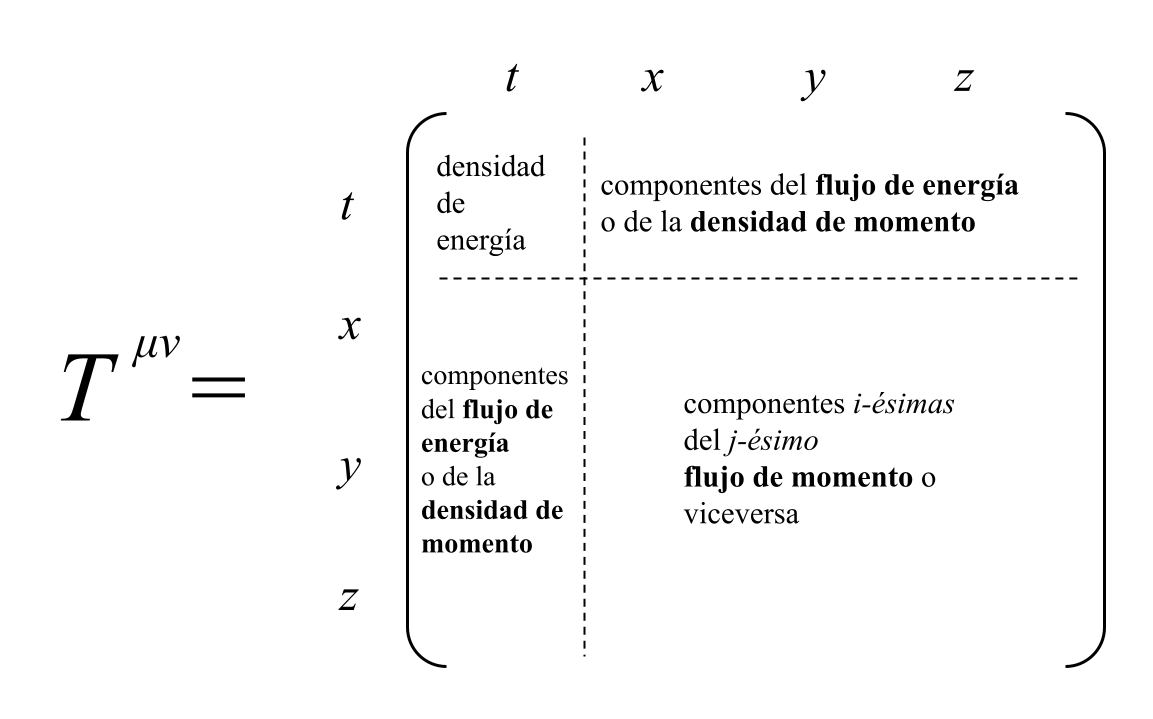
\includegraphics[width=0.85\textwidth]{Im/tensor.png}
\end{remarkbox}

De este tensor vamos a enunciar las siguientes propiedades:
\begin{itemize}
    \item Es \textbf{simétrico}, es decir que:
    $$T^{\mu\nu}=T^{\nu\mu}$$
    \item La \textbf{conservación de energía y flujo de momento} nos garantizan que:
    $$\nabla_{\nu}T^{\mu\nu}=0$$
\end{itemize}

Como vamos a estudiar la ecuación de campo de un agujero negro con carga eléctrica (Reissner-Nordström), vamos a buscar el tensor de estrés energía para un campo electromagnético.

\begin{remarkbox}{Tensor de Estrés-Energía Electromagnético}

    Recordemos primero el \textbf{tensor de campo electromagnético} $F^{\mu\nu}$:
    \begin{equation}
    F_{\alpha\beta}=
    \begin{pmatrix}
    0 & E_1/c & E_2/c & E_3/c\\
    -E_1/c & 0 & -B_3 & B_2\\
    -E_2/c & B_3 & 0 & -B_1\\
    -E_3/c & -B_2 & B_1 & 0
    \end{pmatrix}
    \label{tensorcampoelectromagnetico}
    \end{equation}

    Sabemos además que, para un campo EM, la \textbf{densidad de energía} está dada por:
    $$\rho_E=\frac{1}{2\mu_0}\left(E^2+B^2\right)$$
    
    Como los campos EM almacenan energía, tienen que tener un tensor de stress-energía asociado. Los únicos elementos que intervienen aquí son los campos electromagnéticos y el espacio-tiempo, por lo que $T^{\mu\nu}$ (simétrico) deberá ser una combinación de $F^{\mu\nu}$ (antisimétrico) y $g_{\mu\nu}$ (simétrico). Tomando esto en cuenta, y además pidiendo que la entrada $tt$ corresponda a la densidad de energía $\rho_E$ de más arriba, podemos llegar al siguiente tensor:
    \begin{equation}
    T^{\mu\nu}=\frac{1}{\mu_0}\left(\frac{1}{4}g^{\mu\nu}F^{\sigma\gamma}F_{\sigma\gamma}-F^{\mu\alpha}g_{\alpha\beta}F^{\nu\beta}\right)
    \label{tensorestresenergiafunciondeF}
    \end{equation}
    
    
    Una característica destacable de este tensor es que es \textbf{traceless} (traza nula). Es decir que, si bajamos un índice y contraemos, podemos demostrar que:
    
    \begin{equation}
        T\equiv T^{\alpha}_{\alpha}=0
        \label{traceless}
    \end{equation}
\end{remarkbox}

\newpage

\section{\huge{Ecuaciones de Campo de Einstein}}

\textcolor{myred}{\hrule}

\newthought{Ya obtuvimos} lo que va al lado derecho de las ecuaciones de campo. Lo que nos queda por hacer es construir el lado izquierdo de la misma. Evidentemente, el dado izquierdo también deberá:

\begin{itemize}
    \item Ser un \textbf{tensor contravariante de segundo rango}, al que llamaremos $G^{\mu\nu}$, tal que:
    
    $$G^{\mu\nu}=k T^{\mu\nu}$$
    
    ($k$ es una constante de proporcionalidad a determinar).
    
    \item Ser \textbf{simétrico}, es decir que $G^{\mu\nu}=G^{\nu\mu}$.
    \item Tener \textbf{gradiente absoluto nulo}, es decir $\nabla_{\mu}G^{\mu\nu}=0.$
    \item Representar la \textbf{curvatura} del espacio-tiempo, es decir que deberá \textbf{contener derivadas segundas del tensor métrico} $g_{\mu\nu}$.
    \item Reducirse a la fórmula newtoniana $\nabla^2\Phi=4\pi G \rho$ en el límite no-relativista.
\end{itemize}

Una primer propuesta que podríamos hacer es utilizar el \textbf{tensor de Ricci} (que, si recordamos, era una contracción del tensor de Riemann, el cual contiene toda la información necesaria para describir la curvatura del espacio-tiempo). Si bien este tensor es simétrico, el problema yace en que, en general, $\nabla_\mu R^{\mu\nu}\neq0$, por lo que tendremos que proponer algo distinto.

\vspace{0.5cm}

¿Qué otras cosas podemos agregar? Los únicos elementos razonables podrían ser otras contracciones del tensor de Riemann (por ejemplo, el escalar de curvatura $R$), y el propio tensor métrico $g^{\mu\nu}$. La forma más general de combinar esto (respetando el requisito de simetría) es la siguiente:

$$G^{\mu\nu}=R^{\mu\nu}+b g^{\mu\nu} R+\Lambda g^{\mu\nu}$$

Donde $b$ y $\Lambda$ son constantes (escalares).

Si pedimos que, además, $\nabla_{\nu}G^{\mu\nu}=0$, tenemos que:

\begin{equation}
\begin{split}
\nabla_{\nu}G^{\mu\nu}&=\nabla_{\nu}\left(R^{\mu\nu}+b g^{\mu\nu} R+\Lambda g^{\mu\nu}\right)=\\
&=\nabla_{\nu}\left(R^{\mu\nu}+b g^{\mu\nu} R\right)=0
\end{split}
\end{equation}

\begin{marginfigure}
\begin{remarkbox}{Identidad de Bianchi}
$$\nabla_\sigma R_{\alpha\beta\mu\nu}+\nabla_\nu R_{\alpha\beta\sigma\mu}+$$ $$\nabla_\mu R_{\alpha\beta\nu\sigma}=0$$
\end{remarkbox}
\end{marginfigure}

Si utilizamos la \textbf{identidad de Bianchi}, podemos demostrar que es necesario que $b=-\frac{1}{2}$. La ecuación toma entonces la forma:

\begin{equation}
    R^{\mu\nu}-\frac{1}{2} g^{\mu\nu} R+\Lambda g^{\mu\nu}=k T^{\mu\nu}
\end{equation}

Podemos utilizar ahora el requisito de que la ecuación se reduzca a la newtoniana en el límite no-relativista para determinar el valor de la constante $k$. Esto consiste en considerar el \textbf{límite de campo débil}\cite[][p.255]{moore}, e implementar las desviaciones geodésicas. Nos saltearemos esta deducción\cite[][p.246]{moore} para concluir que es necesario que $k=8\pi G$. Las ecuaciones de campo son entonces:

\begin{marginfigure}
\begin{remarkbox}{Weak-Field Limit}
El \textbf{Límite de Campo Débil} consiste en proponer un tensor métrico que difiere muy levemente del $\eta_{\mu\nu}$ del espacio de Minkowski. Es posible demostrar, mediante un análisis perturbativo, que en dicho límite la entrada $g_{00}$ del tensor métrico tiene la forma:

\begin{equation}
    g_{00}=1-\frac{2GM}{c^2 r}
    \label{g00}
\end{equation}

Que está íntimamente relacionada con el potencial gravitatorio newtoniano.
\end{remarkbox}
\end{marginfigure}

\begin{remarkbox}{Ecuaciones de Campo de Einstein}
\begin{equation}
    R^{\mu\nu}-\frac{1}{2} g^{\mu\nu} R+\Lambda g^{\mu\nu}=8 \pi G T^{\mu\nu}
\end{equation}
\end{remarkbox}

La constante $\Lambda$ se llama \textbf{constante cosmológica}, y en los análisis posteriores podemos considerarla igual a cero.

Multiplicando por el tensor métrico y contrayendo un par de índices, podemos llegar a una forma alternativa para las ecuaciones:

\begin{remarkbox}{Ecuaciones de Campo de Einstein - Forma Alternativa}
\begin{equation}
    R^{\mu\nu}=8 \pi G\left(T^{\mu\nu}-\frac{1}{2} g^{\mu\nu} T\right)+\Lambda g^{\mu\nu}
    \label{campoeinsteincontravariante}
\end{equation}
\end{remarkbox}

\newpage

\section{\huge{Geodésicas}}
\textcolor{myred}{\hrule}
\begin{flushright}
\textit{It took the light,\\ absolutely forever to get to your eyes.\\\textbf{Alex Turner}}
\end{flushright}

\newthought{Ya sabemos a la perfección cómo es que la energía modifica la geometría del espacio-tiempo}. Lo que nos queda por explicar ahora es cómo un objeto se mueve en este espacio-tiempo curvado, para poder hallar ecuaciones diferenciales de movimiento. 

Para esto, vamos a definir una \textbf{geodésica} como la \textbf{curva entre dos eventos con el mayor tiempo propio}. La hipótesis geodésica dice que, en los espacio-tiempos con cualquier tipo de geometría (incluso curvados), los cuerpos libres de fuerzas se mueven en geodésicas. Es decir que, al viajar de un punto $A$ a un punto $B$ en el espacio-tiempo, de todas las posibles trayectorias los cuerpos 'eligen' la que hace que sus relojes midan más tiempo propio.

Veamos qué se puede hacer con esta hipótesis.

\subsection*{\textbf{Geodésicas Timelike}}

\begin{marginfigure}
\captionsetup{type=figure}
    \centering
    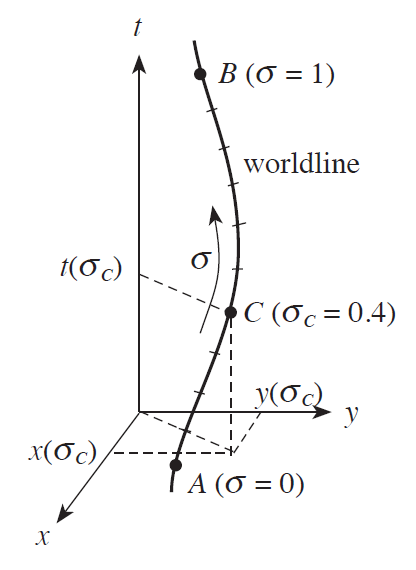
\includegraphics[width=1.3\textwidth]{Im/geod.png}
    \caption{Podemos describir la curva (worldline) entre dos eventos $A$ y $B$ etiquetando todos los eventos entre ellos mediante un parámetro $\sigma$, luego especificando las coordenadas espaciales y temporales de dichos eventos como función de dicho parámetro.}
    \label{fig:sen}
\end{marginfigure}

Tomemos dos eventos $A$ y $B$ que tienen una separación de tipo \textit{timelike} (es decir con $ds^2>0$, el movimiento de las partículas con masa, que viajan a velocidades inferiores a la de la luz). Pensemos en las posibles trayectorias que conectan los dos eventos, y hagámoslas variar con un parámetro $\sigma$, que va de $0$ a $1$. Es decir, vamos a especificar $x^{\mu}(\sigma)$ a lo largo de la trayectoria. El tiempo propio a lo largo de esta trayectoria va a estar dado por:

\begin{equation}
    \tau_{AB}=\int \sqrt{-ds^2}=\int_0^1\sqrt{-g_{\mu\nu}(x^{\alpha}(\sigma))\frac{dx^\mu}{d\sigma}\frac{dx^\nu}{d\sigma}}d\sigma
\end{equation}

Hallar la curva que maximice el valor de $\tau_{AB}$ es muy similar a cuando, en Mecánica Clásica, buscamos la trayectoria $q_i(t)$ que \textbf{minimice la acción $S$}, la cual estaba definida como:

$$S\equiv \int_{t_a}^{t_b}L(q_i,\Dot{q}_i)dt$$

Donde $L$ es el \textbf{lagrangiano} del sistema, una función de las coordenadas generalizadas y las velocidades generalizadas. A partir de este principio variacional, llegábamos a las \textbf{Ecuaciones de Euler-Lagrange}:

\begin{equation}
    \frac{d }{dt}\left(\frac{\partial L}{\partial \dot{q}_i}\right)-\frac{\partial L}{\partial q_i}=0
\end{equation}

La situación aquí es completamente análoga. Podemos armar un lagrangiano que depende de las posiciones $x^{\mu}$ y las 'velocidades' $\dot{x}^\mu \equiv d x^\mu / d\sigma$:

\begin{remarkbox}{Lagrangiano}
\begin{equation}
    L(x^{\alpha},\dot{x}^{\alpha})\equiv\sqrt{-g_{\mu\nu}(x^{\alpha})\dot{x}^{\mu}\dot{x}^{\nu}}
\end{equation}
\end{remarkbox}

Que, de igual manera, nos conducen a las ecuaciones:

\begin{remarkbox}{Ecuaciones de Euler-Lagrange}
\begin{equation}
    \frac{d }{d\sigma}\left(\frac{\partial L}{\partial \dot{x}^{\alpha}}\right)-\frac{\partial L}{\partial x^{\alpha}}=0
\end{equation}
\end{remarkbox}

Se puede proceder reemplazando el lagrangiano y derivando, y luego de un buen trabajo algebraico, llegamos a la siguiente ecuación:

\begin{remarkbox}{Ecuación geodésica}
\begin{equation}
\frac{d}{d\tau}\left(g_{\alpha\beta}\frac{dx^{\beta}}{d\tau}\right)-\frac{1}{2}\partial_\alpha g_{\mu\nu}\frac{dx^{\mu}}{d\tau}\frac{dx^{\nu}}{d\tau}=0
\end{equation}
\end{remarkbox}

Esta ecuación es muy conveniente, ya que utiliza el tensor métrico de forma explícita, en lugar de tenerlo 'oculto' en el lagrangiano. También nos hemos independizado del parámetro $\sigma$, aunque a veces nos será conveniente volver a dicho parámetro arbitrario, como es en el caso de las geodésicas \textit{lightlike}, es decir la trayectoria de fotones. Para cualquier trayectoria, el $\tau_{AB}$ de la luz es siempre cero (podríamos decir que \textit{un reloj moviéndose a la velocidad de la luz no avanza}), por lo que $\tau$ deja de ser un buen parámetro.

También es posible utilizar los \textbf{símbolos de Christoffel} para reescribir la ecuación geodésica. Esta se lee:

\begin{remarkbox}{Ecuación geodésica - Forma Alternativa}
\begin{equation}
\frac{d^2x^{\mu}}{d\tau^2}+\Gamma^{\mu}_{\alpha\beta}\frac{dx^{\alpha}}{d\tau}\frac{dx^{\beta}}{d\tau}=0
\label{geodesicx}
\end{equation}
\end{remarkbox}

\begin{figure}
    \centering
    
\includegraphics[width=0.6\textwidth]{Im/sonic.jpg}
    \caption{El único meme que pusimos en este trabajo.}
    \label{fig:my_label}
\end{figure}






%Einstein Field equation
%\chapter{\textcolor{myred}{La métrica de Reissner-Nordström}}

%Principio de equivalencia (fuerte): En un laboratorio en caída libre (no rotante) que ocupa una pequeña región del espacio tiempo, las leyes de la física son las correspondientes a la relatividad especial

\section{\huge{Resolviendo la ecuación de Einstein}}

\textcolor{myred}{\hrule}

\newthought{En los capítulos} anteriores hemos definido una buena cantidad de conceptos y herramientas correspondientes a la teoría de la Relatividad General. En este capítulo, buscaremos una solución a la ecuación de campo de Einstein-Maxwell para un cuerpo\footnote{Notesé como nos referimos a un cuerpo con ciertas características, no a un agujero negro en particular.} puntual con carga. 

\newthought{El primer paso} para resolver la ecuación de campo de Einstein es definir un buen sistema de coordenadas. Hemos visto en los capítulos anteriores que la geometría del espacio-tiempo alrededor de una distribución de masa y energía está determinada por dicha ecuación. No obstante, tenemos libertad para elegir las coordenadas que utilicemos para describir dicha geometría. Como hacemos siempre en Física, utilizaremos un sistema de coordenadas que explote las simetrías del problema que estemos resolviendo. Luego teniendo en cuenta, estas simetrías podremos proponer una métrica que contenga la menor cantidad de componentes incógnitas posibles.
\begin{marginfigure}
\begin{extrabox}{}
Los pasos para resolver la ecuación se pueden condensar en:
\begin{itemize}
    \item Usar la simetría del problema para definir un sistema de coordenadas lo más completo posible.
    \item Proponer una métrica con la menor cantidad de coeficientes indeterminados posibles.
    \item Sustituir la métrica de prueba en la ecuación de Einstein.
    \item Resolver el sistema de ecuaciones diferenciales para las componentes incógnitas.
\end{itemize}
\end{extrabox}
\end{marginfigure}
Una vez que tengamos esta métrica de prueba la sustituimos en la ecuación de Einstein y obtenemos un sistema de ecuaciones diferenciales acopladas, el cual, si somos capaces de resolverlo, habremos encontrado un sistema de coordenadas que describe la geometría buscada, es decir obtuvimos la métrica para del  espacio-tiempo para el sistema estudiado.

\section{\huge{La forma general de una métrica esféricamente simétrica}}

\textcolor{myred}{\hrule}

\subsection*{\textbf{Consideraciones sobre la forma general de la métrica}}

\newthought{Para poder resolver} las ecuaciones, tendremos que asumir ciertas características de la solución:

\vspace{0.75cm}

\begin{remarkbox}{Consideraciones sobre la métrica de Reissner-Nordström}
\begin{itemize}
    \item Consideramos el espacio tiempo alrededor de una fuente esféricamente simétrica.
    \item El espacio es vacío excepto por la presencia de campos electromagnéticos.
    \item Cuando la carga del cuerpo tiende a 0 $(Q \to 0)$ la métrica debe ser la de Schwarzchild.
    \item Cuando la distancia al objeto tiende a infinito $(r \to \infty)$ la métrica debe acercarse a la de Minkowski.
\end{itemize}
\end{remarkbox}

\subsection*{\textbf{Elección de las coordenadas espaciales}}

Simetría esférica significa que podemos definir un conjunto anidado de superficies bidimensionales concéntricas en el espacio-tiempo alrededor de la fuente cuya geometría intrínseca es la misma que la de una esfera ordinaria en dos dimensiones. Si definimos las coordenadas angulares $\theta$ (ángulo polar) y $\phi$ (ángulo azimutal) en la forma usual para cada superficie, y definimos $r$ como la circunferencia de tal esfera dividida por $2\pi$. Luego la métrica para cada superficie esférica es 
\begin{equation}
    ds^2 = r^2(d\theta^2+\sin^2{\theta}d\phi^2)
    \label{metricaRN1}
\end{equation}

Esta ''parte'' de la métrica solo aplica para una de las esferas anidadas ($r$ constante), es decir tenemos las componentes del tensor métrico que tienen que ver con las coordenadas angulares. Hasta ahora no hay nada que nos prohiba darle a cada esfera su propio set de coordenadas angulares. Pero podemos alinear los sistemas coordenados de todas las esferas concéntricas, pidiendo que la linea curva definida por $\theta = cte$ y $\phi=cte$ sean perpendiculares a cada esfera. Esto significa que los vectores $\bm{e}_\theta$ y $\bm{e}_\phi$ sean perpendiculares a $\bm{e}_r$. Recordando \ref{tensormetricobases} lo anterior nos dice que
\begin{equation*}
    g_{r\theta} = \bm{e}_r  \cdot \bm{e}_\theta = 0 \hspace{1cm} g_{r\phi} = \bm{e}_r  \cdot \bm{e}_\phi =0
\end{equation*}
Entonces, tenemos las componentes del tensor métrico que tienen que ver con $r$, donde $g_{rr}$ es incógnita por ahora y podemos escribir la parte puramente espacial de la métrica
\begin{equation}
    ds^2 = g_{rr}dr^2 + r^2(d\theta^2+\sin^2{\theta}d\phi^2)
    \label{metricaRN2}
\end{equation}

Ahora, supongamos que tenemos un término de la métrica que sea de la forma $g_{t\phi}dtd\phi$, esto implicaría que la geometría del espacio tiempo trata a los desplazamientos dondo $d\phi > 0$ distinto a los desplazamientos donde $d\phi <0$. Esto daría una dirección preferencial al movimiento contrario a la suposición de simetría esférica\footnote{La métrica de Kerr para agujeros negros rotantes, donde no hay simetría esférica esta componente del tensor no es nula, lo cual complica considerablemente las cosas.}. Entonces, la simetría esférica del sistema nos permite elegir usar coordenadas de modo tal que $g_{t\phi}=0$. Por un argumento, similar $g_{t\theta}=0$. Finalmente la métrica que tiene en cuenta el espacio y el tiempo tiene la forma 
\begin{equation}
    ds^2 = g_{tt}dt^2 + 2g_{rt}drdt +g_{rr}dr^2 + r^2(d\theta^2+\sin^2{\theta}d\phi^2)
\end{equation}
donde escribimos $2g_{rt}drdt$ por la simetría del tensor métrico. 

\subsection*{\textbf{Elección de la coordenada temporal}}

Hasta ahora la coordenada temporal es completamente arbitraria. Podemos usar nuestra libertad en la elección de las coordenadas para definir $g_{tt}$ y $g_{rt}$, pero teniendo cuidado que hay ciertas restricciones. Primero, $g_{tt} \neq 0$ o si no, no tendríamos espacio-\textit{tiempo}. Segundo, debe ser negativo cuando las otras componentes de la métrica son positivos y $g_{tr}=0$ (para que exista el caso lightlike $ds^2=0$). Supongamos que realizamos alguna elección arbitraria de las coordenadas temporales que definen $g_{tt}$ y utilizamos las ecuaciones de Einstein para encontrar $g_{rt}$. Si realizamos una transformación de coordenadas de la forma 
\begin{equation*}
    t' = t + f(r,t)
\end{equation*}
se puede demostrar que una elección apropiada de dicha función setea $g'_{rt}=0$ en nuestro sistema de coordenadas transformado\footnote{El ' significa en el sistema transformado, no derivada con respecto a algo.}. Pero si podemos elegir una coordenada temporal de modo tal que se cumpla $g'_{rt}=0$, por la arbritrariedad en la elección podemos elegir directamente $g_{rt}=0$ antes de resolver la ecuación de Einstein.\footnote{Eliminar elementos de la diagonal representa una gran ventaja a la hora de realizar los cálculos.}.

Finalmente, una forma general para la métrica esféricamente simétrica es
\begin{remarkbox}{Forma general para una métrica esféricamente simétrica }
\begin{equation*}
    ds^2 = A(r,t)dt^2 - B(r,t)dr^2 - r^2d\theta^2 -r^2\sin^2{\theta}d\phi^2
\end{equation*}
\end{remarkbox}

donde elegimos $\phi$ y $\theta$ como las coordenadas angulares azimutal y polares de siempre, $r$ como la coordenada radial circunferencial, y $t$ de modo tal que $g_{rt}$.

\section{\huge{Reemplazando la forma general de la métrica en la ecuación de Einstein}}

\newthought{Siguiendo} la 'receta' que presentamos antes, ahora debemos utilizar la forma de la métrica que hallamos y reemplazarla directamente en la ecuación de campo de Einstein que recordemos está dada por (\ref{campoeinsteincontravariante}), tomando la constante cosmológica como $0$ tenemos\footnote{Hemos agregado un término $c^{-4}$ que antes no estaba por simplicidad de las cuentas pero ahora nos será útil trabajar en el Sistema Internacional de Unidades (SI).}
\begin{equation*}
R^{\mu\nu}= \frac{8 \pi G}{c^4}\left(T^{\mu\nu}-\frac{1}{2} g^{\mu\nu} T\right)
\end{equation*}
Además, recordando que estamos trabajando en el vacío (solo con presencia de campos electromagnéticos), el tensor de energía-momento está dado por (\ref{tensorestresenergiafunciondeF})
\begin{equation*}
T^{\mu\nu}=\frac{1}{4\pi k}\left(\frac{1}{4}g^{\mu\nu}F^{\sigma\gamma}F_{\sigma\gamma}-F^{\mu\alpha}g_{\alpha\beta}F^{\nu\beta}\right)
\end{equation*}
y para este tensor calculamos que su traza era nula (ec. \ref{traceless}), por lo que la ecuación de campo de Einstein que usaremos es
\begin{equation}
R^{\mu\nu}=\frac{8 \pi G}{c^4}T^{\mu\nu}
\label{riccicosmonula}
\end{equation}
\subsection*{\textbf{Bajar los índices 'upstairs' a 'downstairs'}}

En esta sección expresaremos el tensor de estrés-energía (ec. \ref{tensorestresenergiafunciondeF} y el tensor de Ricci (ec. \ref{riccicosmonula}) de forma covariante (con los índices abajo \textit{downstairs}), dado que nos será útil más adelante. 

Para bajar dichos índices multiplicamos a ambos lados por el tensor métrico\begin{marginfigure}
\begin{extrabox}{}
Para bajar o subir índices una regla que funciona es pensar que el segundo índice del tensor métrico índica qué índice del tensor sube o baja (es el que está repetido) y el primer índice del tensor métrico indica por qué índice se remplaza. Por ejemplo:
\begin{equation}
    g^{\alpha\gamma} R_{\alpha\beta\gamma\sigma} = {{R_{\alpha\beta}}^\alpha}_\sigma
\end{equation}
\end{extrabox}
\end{marginfigure} de forma conveniente entonces para el tensor de Ricci por ejemplo:
\begin{equation}
\begin{split}
g_{\alpha\mu}g_{\beta\nu}R^{\mu\nu} &= \frac{8 \pi G}{c^4}g_{\alpha\mu}g{\beta\nu}T^{\mu\nu} \\    
g_{\alpha\mu}R^{\mu}_\beta &= \frac{8 \pi G}{c^4}g_{\alpha\mu}T^{\mu}_\beta \\    
R_{\alpha\beta} &= \frac{8 \pi G}{c^4}T_{\alpha\beta}   
\end{split}
\label{riccidownstairs}
\end{equation}
De manera similar podemos bajar los indices del tensor de estrés-energía
\begin{equation}
T_{\alpha\beta}=\frac{1}{\mu_0}\left(\frac{1}{4}g_{\alpha\beta}F_{\mu\nu}F^{\mu\nu}-g_{\beta\nu}F_{\alpha\mu}F^{\nu\mu}\right)
\label{tensorestresdownstairs}
\end{equation}

\subsection*{\textbf{Cálculo del tensor de Ricci}}

Comencemos por el lado izquierdo de la ecuación de Einstein en forma covariante (\ref{riccidownstairs}), es decir por el cálculo del tensor de Ricci. Para calcular las componentes de dicho tensor debemos primero calcular los símbolos de Christoffel a partir de la ecuación (\ref{simboloChristoffel}) 
\begin{equation*}
\Gamma^{\alpha}_{\mu \nu}=\frac{1}{2}g^{\alpha\sigma}\left[\partial_{\mu}g_{\nu\sigma}+\partial_{\nu}g_{\sigma \mu}-\partial_{\sigma}g_{\mu\nu}\right]
\end{equation*}

Por lo que necesitamos el tensor métrico en su forma covariante y contravariante. Hasta ahora, a partir de la métrica que tenemos $g_{\mu\nu}$ y $g^{\mu\nu}$ son\footnote{Ya vimos que en la representación matricial son matrices inversas.} 
\begin{equation}
g_{\mu\nu} = \begin{pmatrix}
Ac^2 & 0 & 0 & 0 \\
0 & -B & 0 & 0 \\
0 & 0 & -r^2 & 0 \\
0 & 0 & 0 & -r^2\sen^2{\theta}
\end{pmatrix}
\hspace{0.2cm}
g^{\mu\nu} = \begin{pmatrix}
\frac{1}{Ac^2} & 0 & 0 & 0 \\
0 & \frac{-1}{B}  & 0 & 0 \\
0 & 0 & \frac{-1}{r^2}  & 0 \\
0 & 0 & 0 & \frac{-1}{r^2\sen^2{\theta}} 
\end{pmatrix}
\label{tensoresmetricos}
\end{equation}

Veamos que para calcular los símbolos de Christoffel solo debemos calcular las derivadas parciales de las entradas del tensor métrico y ser muy prolijos con los índices. Esta tarea no es para nada difícil, pero sí muy larga y tediosa. A modo de ejemplo, mostramos en el apéndice ... el cálculo del símbolo ..... Esta tarea por suerte puede ser simplificada mediante métodos computacionales\cite[][p. 26]{Jhonny} y los símbolos de Christoffel no nulos resultan\footnote{Existen varios softwares que permiten el cálculo de simbolos de Christoffel, tensores de Ricci, de Riemann. Maple 17 es un software que permite realizar este tipo de cálculo para entradas incógnitas como los A y B que tenemos, lamentablemente es privado. Einstein.py es un paquete de Python de carácter libre que también permite realizar este tipo de cálculos, pero (hasta donde sabemos) solo para métricas ya dadas. Es decir, no podemos realizar derivadas simbólicas para los $A$ y $B$ que necesitamos.} 

\begin{equation}
\begin{split}
&\Gamma^{0}_{00} = \frac{\dot{A}}{2Ac} \hspace{1cm} \Gamma^{1}_{01} = \Gamma^{1}_{10} = \frac{\dot{B}}{2Bc} \\
&\Gamma^{0}_{11} = \frac{\dot{B}}{2Ac} \hspace{1cm} \Gamma^{0}_{01} = \Gamma^{0}_{10} = \frac{A'}{2A} \\
&\Gamma^{1}_{00} = \frac{A'}{2B} \hspace{1cm} ~~\Gamma^{2}_{12} = \Gamma^{2}_{21} = \frac{1}{r} \\
&\Gamma^{1}_{11} = \frac{B'}{2B} \hspace{1cm} ~~\Gamma^{3}_{13} = \Gamma^{3}_{31} = \frac{1}{r} \\
&\Gamma^{1}_{22} = -\frac{r}{B} \hspace{1cm} ~\Gamma^{3}_{23} = \Gamma^{3}_{32} = \cot{\theta} \\
&\Gamma^{1}_{33} = -\frac{r\sen^2{\theta}}{B} \hspace{0.5cm} \Gamma^{2}_{33} = -\sen{\theta}\cos{\theta} \\
\end{split}
\end{equation}

donde las primas son derivaciones con respecto a $r$ y los puntos con respecto a $t$.

Luego a partir de la definición del tensor de Riemann (ec. \ref{riemann}) 
\begin{equation*}
R^\mu_{\alpha \nu \beta}\equiv\partial_{\nu}\Gamma^{\mu}_{\alpha \beta}-\partial_{\beta}\Gamma^{\mu}_{\alpha\nu}+\Gamma^{\mu}_{\nu\gamma}\Gamma^{\gamma}_{\alpha\beta}-\Gamma^{\mu}_{\beta\gamma}\Gamma^{\gamma}_{\alpha\nu}
\end{equation*}
y del tensor de Ricci (ec. \ref{ricci}) 
\begin{equation*}
R_{\alpha\beta} \equiv R^\mu_{\alpha \mu \beta}
\end{equation*}

Lo único que tenemos que hacer para obtener el tensor de Ricci en función de los símbolos de Christoffel es intercambiar los $\nu$ por $\mu$ y obtenemos
\begin{equation}
R^\mu_{\alpha \mu \beta}= R_{\alpha\beta}= \partial_{\mu}\Gamma^{\mu}_{\alpha \beta}-\partial_{\beta}\Gamma^{\mu}_{\alpha\mu}+\Gamma^{\mu}_{\mu\gamma}\Gamma^{\gamma}_{\alpha\beta}-\Gamma^{\mu}_{\beta\gamma}\Gamma^{\gamma}_{\alpha\mu}    
\end{equation}
y entonces los simbolos de Ricci son:
\begin{equation}
\begin{split}
R_{00} &= -\frac{A'}{4B}\biggr(\frac{A'}{A}+\frac{B'}{B}\biggr)+\frac{A''}{2B}+\frac{A'}{Br}-\frac{\Ddot{B}}{2Bc^2}+\frac{\dot{B}}{4Bc^2}\biggr(\frac{\dot{A}}{A}-\frac{\dot{B}}{B}\biggr) \\
R_{11} &= \frac{A'}{4A}\biggr(\frac{A'}{A}+\frac{B'}{B}\biggr)-\frac{A''}{2A}+\frac{B'}{Br}-\frac{\Ddot{B}}{2Ac^2}-\frac{\dot{B}}{4Ac^2}\biggr(\frac{\dot{A}}{A}-\frac{\dot{B}}{B}\biggr) \\
R_{22} &= -\frac{r}{2B}\biggr(\frac{A'}{A}-\frac{B'}{B}\biggr)-\frac{1}{B}+ 1 \\
R_{33} &= \biggr[-\frac{r}{2B}\biggr(\frac{A'}{A}-\frac{B'}{B}\biggr)-\frac{1}{B}+ 1 \biggr]\sin^2{\theta} = R_{22}\sin^2{\theta}\\
R_{01} &= R_{10} = \frac{\dot{B}}{Brc} \\
\end{split}
\end{equation}

\newthought{Hasta aquí} es lo máximo que podemos generalizar el campo gravitacional esféricamente simétrico. Para determinar $A$ y $B$ necesitaremos resolver el lado derecho de la ecuación de Einstein utilizando el tensor de energía-momento y luego comparar con el lado izquierdo. 

\subsection*{\textbf{Cálculo del Tensor de Estrés-Energía}}
En nuestro caso, solo hay campos eléctricos en el espacio, y sabemos de la simetría esférica del problema que el campo solo puede tener componente radial y que dicha componente solo no puede depender de $\phi$ o $\theta$, entonces
\begin{equation}
    E_1=E_r(t,r)=cF_{01}=-cF_{10}
\end{equation}
El tensor de campo electromagnético dado por (\ref{tensorcampoelectromagnetico}) queda como
\begin{equation}
    F_{\alpha\beta}=
    \begin{pmatrix}
    0 & E_r/c & 0 & 0\\
    -E_r/c & 0 & 0 & 0\\
    0 & 0 & 0 & 0\\
    0 & 0 & 0 & 0
    \end{pmatrix}
\end{equation}

Y ahora podemos usar (\ref{tensorestresdownstairs}) para calcular las componentes del tensor de estrés-energía. El primer término es
\begin{equation*}
\begin{split}
\frac{1}{4}g_{\alpha\beta}F_{\mu\nu}F^{\mu\nu} &= \frac{1}{4}g_{\alpha\beta}(F_{\mu 0}F^{\mu0} + F_{\mu 1}F^{\mu1})= \frac{1}{4}g_{\alpha\beta}(F_{00}F^{00} + F_{10}F^{10} + F_{0 1}F^{01}+ F_{11}F^{11}) \\
&= \frac{1}{2}g_{\alpha\beta}F_{0 1}F^{01}
\end{split}
\end{equation*}
donde sumamos sobre los índices repetidos, usamos que el tensor $F_{\alpha\beta}$ solo tiene componentes no nulas $F_{10}$ y $F_{01}$ y que es antisimétrico. El segundo término nos da
\begin{equation}
g_{\beta\nu}F_{\alpha\mu}F^{\nu\mu} = g_{\beta\nu}F_{\alpha 0}F^{\nu 0} + g_{\beta\nu}F_{\alpha 1}F^{\nu 1} = g_{\beta 1}F_{\alpha 0}F^{10} + g_{\beta 0}F_{\alpha 1}F^{01}
\end{equation}
y finalmente llegamos a una expresión para el tensor
\begin{equation}
T_{\alpha\beta} = \frac{1}{\mu_0}\biggr(\frac{1}{2}g_{\alpha\beta}F_{0 1}F^{01} - g_{\beta 1}F_{\alpha 0}F^{10} - g_{\beta 0}F_{\alpha 1}F^{01}\biggr)
\end{equation}
A partir de esto obtener las componentes del tensor fácil, simplemente reemplazamos $\alpha$ y $\beta$ por todas las combinaciones posibles entre $0$ y $3$ y reemplazamos las entradas del tensor $g_{\alpha\beta}$ según (\ref{tensoresmetricos}) y obtenemos que los únicos 4 términos no nulos 
\begin{equation}
\begin{split}
T_{00} &= \frac{1}{\mu_0}\biggr(\frac{1}{2}g_{00}F_{01}F^{01} - g_{00}F_{01}F^{01}\biggr)= -\frac{1}{2\mu_0}AF_{01}F^{01}\\
T_{11} &=\frac{1}{2\mu_0}B F_{01}F^{01}\\
T_{22} &= -\frac{1}{2\mu_0}r^2 F_{01}F^{01} \\
T_{33} &= \frac{1}{2\mu_0}r^2 \sen^2{\theta} F_{01}F^{01} = T_{22}\sen^2{\theta}
\end{split}
\label{componentestensorestresenergia}
\end{equation}

Ahora que tenemos ambos lados de la ecuación de Einstein estamos en condiciones de comparar el tensor de Ricci con el de energía-momento para poder finalmente calcular $A$ y $B$ y obtener nuestra métrica.

\subsection*{\textbf{Comparación tensor de Ricci y de Estrés-Energía}}

Es fácil, ver de la ecuación de campo que si una entrada en el tensor de Ricci es nula lo será en el de estrés-energía y viceversa. Por ejemplo, la entrada $T_{01}$ es nula entonces la entrada $R_{01}$ deberá serlo y de la ecuación para $R_{01}$ podemos concluir que
\begin{equation}
    \dot{B} = 0 
\end{equation}
$B$ no depende de $t$.

Por otro lado, de (\ref{componentestensorestresenergia}) podemos ver que se cumple
\begin{equation}
    \frac{T_{00}}{A} + \frac{T_{11}}{B} = 0 
\end{equation}
Como sabemos que cada coordenada de $R_{\alpha\beta}$ es una constante multiplicada por $T_{\alpha\beta}$ (ec. \ref{riccidownstairs}) podemos escribir
\begin{equation}
\frac{R_{00}}{A} + \frac{R_{11}}{B} = \frac{1}{rB}\biggr(\frac{A'}{A}+\frac{B'}{B}\biggr) = 0 
\end{equation}
lo cual implica que 
\begin{equation}
0 = \biggr(\frac{A'}{A}+\frac{B'}{B}\biggr) \Rightarrow  \frac{1}{AB}(A'B+AB') = \frac{\partial}{\partial r} \ln(AB)
\end{equation}
entonces $AB$ debe ser constante con respecto a $r$ y lo podemos escribir como 
\begin{equation}
    AB = f(t)
\end{equation}
La relación entre $F_{01}$ downstairs y $F^{01}$ upstairs está dada por
\begin{equation}
    F_{01} = g_{00}g_{11}F^{01} = -fF^{01}
\end{equation}
donde usamos que $g_{00}=A$ y $g_{11}=-B$ y que $AB=f$ 

En este punto necesitamos las ecuaciones de Maxwell en su forma tensorial
\begin{equation}
\begin{split}
\nabla_\beta F^{\alpha\beta} &= 0 \\
\nabla^\mu F^{\alpha\beta} + \nabla^\beta F^{\mu\alpha}  +\nabla^\alpha F^{\beta\mu} &= 0
\end{split}
\end{equation}

donde $\nabla_\gamma$ es la derivada covariante (ó gradiente absoluto) que ya hemos definido en el capítulo anterior.

\begin{marginfigure}
\begin{remarkbox}{Teorema de Birkhoff}
Para demostrar que la función $A$ no depende del tiempo, es posible apelar al siguiente argumento: como sabemos que $AB=f(t)$,  que $\dot{B}=0$, es necesario que $A$ tenga la siguiente forma:

$$A(r,t)=a(r)f(t)$$

Donde $a=k/B$. El coeficiente que acompaña al término $dt^2$ en la métrica será entonces $-Kf(t)g(r)$, de donde concluimos que $Kf(t)$ tiene que ser positivo (para que la \textit{signature} de la métrica nos asegure 3 dimesiones espaciales y una temporal). Esto significa que podemos redefinir la coordenada $t$ como:

\begin{equation}
    dt_{new}=dt_{old}\sqrt{Kf(t)}
\end{equation}

Es decir que la libertad a la hora de elegir la coordenada $t$ nos permite independizarnos del tiempo en la métrica alrededor de un objeto con simetría esférica. Esto es conocido como \textbf{Teorema de Birkhoff}, y si bien aplica a el espacio vacío, también puede generalizarse para incorporar las Ecuaciones de Maxwell en el llamado \textbf{Electrovacío de Reissner-Nordström}.
\end{remarkbox}
\end{marginfigure}


Luego la primera ecuación de Maxwell se escribe como
\begin{equation}
\nabla_\beta F^{\alpha\beta} = \partial_\beta F^{\alpha\beta} + \Gamma^\alpha_{\mu\beta}F^{\mu\beta} + \Gamma^\beta_{\mu\beta}F^{\alpha\mu} = 0 
\end{equation}
Si tomamos $\alpha=1$ en la anterior tenemos 
\begin{equation}
\partial_0 F^{10} + \Gamma^1_{\mu\beta}F^{\mu\beta} + \Gamma^\beta_{\mu\beta}F^{1\mu} = 0
\end{equation}
donde el termino con la derivada $\partial_0$ es el único que sobrevive por las entradas no nulas del $F_{\alpha\beta}$. Veamos la suma implícita en el segundo término
\begin{equation}
\Gamma^1_{\mu\beta}F^{\mu\beta} = \Gamma^1_{\mu0}F^{\mu0} +\Gamma^1_{\mu1}F^{\mu1}= \Gamma^1_{00}F^{00} + \Gamma^1_{10}F^{10} + \Gamma^1_{10}F^{10} + \Gamma^1_{11}F^{11}=0
\end{equation}
Luego este término es nulo porque $\Gamma^1_{01}=\Gamma^1_{10}=F^{00}=F^{11}=0$. Y el tercer término también es nulo 
\begin{equation}
\Gamma^\beta_{\mu\beta}F^{1\mu} = F^{10}(\Gamma^0_{00}+\Gamma^1_{01}+\Gamma^2_{02}+\Gamma^3_{03})=0
\end{equation}
donde los símbolos de Christoffel en el paréntesis se anulan, entonces llegamos a 

\begin{equation}
    \partial_0 F^{10} = 0
\end{equation}
Esto implica, que $F^{10}$ y por lo tanto $E(r)$ no dependen del tiempo y llegamos a 
\begin{equation}
    E_r = E_r(r)
\end{equation}

Si ahora tomamos de entrada el caso $\alpha=0$ 
\begin{equation}
\partial_1 F^{01} + \Gamma^0_{\mu\beta}F^{\mu\beta} + \Gamma^\beta_{\mu\beta}F^{0\mu} = 0
\end{equation}
Procediendo como antes podemos ver que el segundo término desaparece nuevamente pero el tercero no
\begin{equation}
\begin{split}
\Gamma^\beta_{\mu\beta} F^{0\mu} &= \Gamma^\beta_{1\beta} F^{01} = F^{01}(\Gamma^0_{10} +\Gamma^1_{11}+\Gamma^2_{12}+\Gamma^3_{13}) \\
&= F^{01}(\frac{A'}{2A} + \frac{B'}{2B} + \frac{2}{r}) = \frac{2}{r}F^{01} \Rightarrow \\
&\Rightarrow \frac{A'}{2A} + \frac{B'}{2B} = 0 \Rightarrow \frac{1}{2} \biggr(\frac{\partial}{\partial r}\ln(f)\biggr) = 0  
\end{split}
\end{equation}
porque sabíamos que $f(t)$ solo depende de $t$ y luego
\begin{equation}
    0 = \frac{\partial}{\partial r}F^{01} + \frac{2}{r}F^{01}
\end{equation}
Está última ecuación es fácil de resolver integrando 
\begin{equation}
    F^{01} = \frac{C}{r^2}
\end{equation}
donde $C$ es una constante de integración. Lo cual nos permite escribir
\begin{equation}
    E_r = \frac{C}{r^2}
\end{equation}
Podemos utilizar el teorema de Gauss en una superficie Gaussiana esférica y concluir que
\begin{equation}
    E_r = \frac{Q}{4\pi\epsilon_0 r^2}
    \label{Er}
\end{equation}
Esta es esencialmente la ley de Coulomb pero recordemos que $r$ es la circunferencia reducida que \textbf{no necesariamente} mide la distancia radial real en el espacio-tiempo que estamos analizando. 

Ahora solo nos falta expresar $A$ y $B$ como funciones de $r$ y terminamos. Partamos de la siguiente ecuación de Einstein
\begin{equation}
    R_{22} = \frac{8\pi G}{c^4} T_{22}
\end{equation}
Entonces
\begin{equation}
R_{22} = -\frac{r}{2B}\biggr(\frac{A'}{A} - \frac{B'}{B}\biggr) - \frac{1}{B}+1 = -\frac{1}{f}\frac{\partial}{\partial r}(rA) +1
\end{equation}
donde usamos que $f=AB$ y reglas de derivación. Ahora usamos la componente $T_{22}$ del tensor que ya calculamos (ec.\ref{componentestensorestresenergia}) y obtenemos
\begin{equation}
-\frac{1}{f} \frac{\partial}{\partial r}(rA) +1 = \frac{1}{f}\frac{8\pi G}{c^4} \frac{1}{2\mu_0 c^2} r^2 E_r^2
\end{equation}
Reemplazando $E_r$ por (ec. \ref{Er}) 
\begin{equation}
\frac{\partial}{\partial r} (rA) = f - \frac{GQ^2}{4\pi c^6 \mu_0 \epsilon_0^2r^2}
\end{equation}
Si ahora integramos y usamos que $c^2\mu_0= 1/\epsilon_0$ tenemos
\begin{equation}
    A = f + \frac{C_1(t)}{r} + \frac{GQ^2}{4\pi \epsilon_0 c^4 r^2}
    \label{A}
\end{equation}
Ahora, cuando $Q=0$, una de las suposiciones es que la métrica debe reducirse a la de Schwarzchild. Entonces, como mostramos en la ecuación (\ref{g00}), cuando $r$ es muy grande, entramos en límite de campo débil (Weak Field Limit) y $g_{00}$ tiende a 
\begin{equation*}
g_{00} = -1 - \frac{2GM}{c^2 r}
\end{equation*}
Entonces, en este límite, las geodésicas deben estar de acuerdo con el movimiento clásico gravitacional de Newton y mirando (ec. \ref{A}) se debe cumplir que $f=1$ y por lo tanto que 
\begin{equation}
C(t)= -\frac{2GM}{c^2} =- r_s
\end{equation}
que es el famoso \textbf{radio de Schwarzchild}. Además podemos definir 
\begin{equation}
    r_Q^2 = \frac{GQ^2}{4\pi\epsilon_0 c^4}
\end{equation}
y finalmente $A$ y $B$ quedan
\begin{equation}
\begin{split}
A &= 1 - \frac{r_s}{r} + \frac{r_Q^2}{r^2} \\
B &= \biggr(1 - \frac{r_s}{r} + \frac{r_Q^2}{r^2}\biggr)^{-1}
\end{split}
\end{equation}
y el tensor métrico es 

\begin{remarkbox}{Tensor métrico del espacio-tiempo de Reissner-Nordström}
\begin{equation*}
g_{\alpha\beta} = \begin{pmatrix}
\biggr(1 - \frac{r_s}{r} + \frac{r_Q^2}{r^2}\biggr) & 0 & 0 & 0 \\
0 & \biggr(1 - \frac{r_s}{r} + \frac{r_Q^2}{r^2}\biggr)^{-1} & 0 & 0\\
0 & 0 & -r^2 & 0 \\
0 & 0 & 0 & -r^2\sen^2{\theta} \\
\end{pmatrix}
\end{equation*}
\end{remarkbox}

\newthought{Hemos llegado} a la métrica de Reissner-Nordström completa derivada a partir de las ecuaciones de campo de Einstein junto con las ecuaciones de Maxwell. 


\subsection*{\textbf{Sobre las unidades geométricas}}
A partir de ahora, salvo que indiquemos lo contrario, usaremos las unidades geométricas. Esto es, tomaremos la velocidad de la luz $c$, y la constante de gravitación universal $G$ como :

\begin{remarkbox}{Consideración de las unidades geométricas}
\begin{equation*}
    c=G=1\ \ \textit{adimensional}
\end{equation*}
\end{remarkbox}

Hacemos esto para olvidarnos de las constantes, y hacer menos engorrosas las ecuaciones.
\begin{table}[h]
  \begin{center}
    \begin{tabular}{lccl}
      \toprule
      Variable & Unidades SI & Unidades Geom. & Factor \\
      \midrule
      Masa & $kg$ & $m$ &$c^2 G^{-1}$ \\
      Longitud & $m$ & $m$ & 1 \\
      Tiempo & $s$ & $m$ & $c^{-1}$\\
      Velocidad & $m s^{-1}$ & adim & $c$  \\
      Aceleración & $m s^{-2}$ & m{-1} & $c^2$  \\
      Fuerza & $kg m s^{-2}$ & adim & $c^4 G^{-1}$  \\
      Momento Angular & $kg m^2 s^{-1}$ & $m^2$ & $c^3 G^{-1}$ \\
      Momento & $kg m s^{-1}$ & $m$ & $c^3 G^{-1}$ \\
      Energía & $kg m^2 s^{-2}$ & $m$ & $c^{4} G^{-1}$\\
      Densidad de Energía & $kg m^{-1} s^{-2}$ & $m^{-2}$ & $c^4 G^{-1}$  \\
      \bottomrule
    \end{tabular}
  \end{center}
  \caption{Unidades Geométricas. Para convertir Geom. $\rightarrow$ SI, multiplicar por el factor. Para convertir SI $\rightarrow$ Geom., dividir por el factor. De forma general, para unidades SI de ''$kg^\alpha m^\beta s^\gamma$'', las unidades geométricas son ''$m^{\alpha + \beta + \gamma}$''.}
  \label{geounits}
\end{table}
\section{\huge{Geodésicas en la Geometría de Reissner-Nordström}}

\textcolor{myred}{\hrule}

\newthought{Ahora encontremos las ecuaciones que describen el movimiento de fotones y partículas no cargadas.} La partícula seguirá una geodésica \textbf{\textit{time-like}} mientras que el fotón una geodésica \textbf{\textit{light-like}}. Sea $x^\alpha = x^\alpha (\lambda)$ una curva parametrizada por $\lambda$, entonces debe cumplir la Ec. (\ref{geodesicx}):
\begin{equation}
    \frac{d^2 x^\alpha}{d \lambda^2} + \Gamma^\alpha_{\mu\nu} \frac{d x^\mu}{d \lambda} \frac{d x^\nu}{d \lambda} = 0
\end{equation}

Donde $\Gamma^\alpha_{\mu\nu}$ son los símbolos de Christoffel asociados a la métrica. Para una geodésica \textit{time-like} lo más natural es definir el parámetro $\lambda$ como el tiempo propio $\tau$, mientras que una geodésica \textit{light-like} no puede parametrizarse con $\tau$. Mantendremos por ahora el parámetro $\lambda$ para trabajar con los dos casos. Reemplazando los símbolos de Christoffel para nuestra métrica las ecuaciones de movimiento son:
 
\newthought{Para $\alpha=0$:}
\begin{equation}
    \frac{d^2 t}{d \lambda^2} + \frac{A^\prime}{A} \frac{d t}{d \lambda} \frac{d r}{d \lambda} = 0
\label{eqt3.1}
\end{equation}
\newthought{Para $\alpha=1$:}
\begin{equation}
\begin{split}
    \frac{d^2 r}{d \lambda^2} + \frac{A^\prime}{2B} \left(\frac{d t}{d \lambda}\right)^2 + \frac{B^\prime}{2B} \left(\frac{d r}{d \lambda}\right)^2 - \frac{r}{B} \left(\frac{d \theta}{d \lambda}\right)^2 &\\- \frac{r \sin^2{\theta}}{B} \left(\frac{d \phi}{d \lambda}\right)^2 &= 0
\label{eqradial3.1}
\end{split}
\end{equation}
\newthought{Para $\alpha=2$:}
\begin{equation}
    \frac{d^2 \theta}{d \lambda^2} + \frac{2}{r} \frac{d \theta}{d \lambda} \frac{d r}{d \lambda} - \sin{\theta}\cos{\theta} \left(\frac{d \phi}{d \lambda}\right)^2= 0
\end{equation}
\newthought{Para $\alpha=3$:}
\begin{equation}
    \frac{d^2 \phi}{d \lambda^2} + \frac{2}{r} \frac{d \phi}{d \lambda} \frac{d r}{d \lambda} - 2\cot{\theta}\frac{d \phi}{d \lambda} \frac{d \theta}{d \lambda}= 0
\label{eqazimutal3.1}
\end{equation}

Debido a la simetría esférica la trayectoria debe estar contenida en un plano definido por las condiciones iniciales\footnote{Trazamos el plano que contiene la velocidad en el instante inicial, ya sea de la partícula o del fotón. Sí la trayectoria se saliera de ese plano, la dirección en la que lo haga sería preferencial, rompiendo la simetría esférica del sistema.}, por lo que podemos poner sin ninguna pérdida de generalidad que $\theta=\pi/2$ en todo momento. Esto nos anula las derivadas de $\theta$, y las ecuaciones de movimiento se simplifican. Ahora, las Ecs. (\ref{eqradial3.1}) y (\ref{eqazimutal3.1}) nos quedan:

\begin{equation}
    \frac{d^2 r}{d \lambda^2} + \frac{A^\prime}{2B} \left(\frac{d t}{d \lambda}\right)^2 + \frac{B^\prime}{2B} \left(\frac{d r}{d \lambda}\right)^2 -  \frac{r}{B} \left(\frac{d \phi}{d \lambda}\right)^2 = 0
\label{eqradial3.2}
\end{equation}
\begin{equation}
    \frac{d^2 \phi}{d \lambda^2} + \frac{2}{r} \frac{d \phi}{d \lambda} \frac{d r}{d \lambda}= 0
\label{eqazimutal3.2}
\end{equation}

Sí dividimos la Ec. (\ref{eqazimutal3.2}) por $d\phi/d\lambda$, y usamos que:
\begin{equation}
\begin{split}
    \left(\frac{d\phi}{d\lambda}\right)^{-1} \frac{d^2\phi}{d\lambda^2} &= \frac{d}{d\lambda} \log{\left(\frac{d\phi}{d\lambda}\right)}\\
    \text{y, }\ \frac{2}{r} \frac{dr}{d\lambda} &= \frac{d}{d\lambda}\log{(r^2)}
\end{split}
\end{equation}
llegamos a que:

\begin{equation}
    \frac{d}{d\lambda}\log{\left(r^2\frac{d\phi}{d\lambda}\right)}=0 \Rightarrow r^2 \frac{d\phi}{d\lambda} = L = cte
\label{eqL}
\end{equation}

Donde $L$ es una constante del movimiento que coincide con el \textit{momento angular por unidad de masa} de la teoría Newtoniana. De manera similar, obtenemos para la Ec. (\ref{eqt3.1}) que:

\begin{equation}
    \frac{d}{d\lambda}\log{\left(A\frac{dt}{d\lambda}\right)}=0 \Rightarrow A \frac{dt}{d\lambda} = e = cte
\label{eqe}
\end{equation}

Con $e$ una constante del movimiento que se puede interpretar como la \textit{energía total relativista por unidad de masa}. Ahora usamos las Ecs. (\ref{eqL}) y (\ref{eqe}) en la Ec. (\ref{eqradial3.2}) y tenemos:

\begin{equation}
    \frac{d^2 r}{d \lambda^2} + \frac{A^\prime}{2B} \frac{e^2}{A^2} + \frac{B^\prime}{2B} \left(\frac{d r}{d \lambda}\right)^2 - \frac{r}{B} \frac{L^2}{r^4} = 0
\end{equation}
recordando que $B\prime=-A\prime/A^2$ y multiplicando por $2Bdr/d\lambda$:
\begin{equation}
\begin{split}
    0&=2B\frac{d^2 r}{d \lambda^2}\frac{dr}{d\lambda} - e^2 B^\prime \frac{dr}{d\lambda} + B^\prime \frac{dr}{d\lambda} \left(\frac{d r}{d \lambda}\right)^2 - \frac{2L^2}{r^3} \frac{dr}{d\lambda}\\
    &=\frac{d}{d\lambda}\left[ B \left(\frac{d r}{d \lambda}\right)^2 - e^2 B + \frac{L^2}{r^2}\right]
\end{split}
\end{equation}
por lo que:
\begin{equation}
    B \left(\frac{d r}{d \lambda}\right)^2 - e^2 B + \frac{L^2}{r^2} = -(e_0)^2 = cte
\label{eqe0}
\end{equation}

Donde $e_0$ se puede pensar como la \textit{energía total en reposo por unidad de masa}. Reescribiendo la Ec. (\ref{eqe0}) obtenemos:
\begin{equation}
    \left(\frac{d r}{d \lambda}\right)^2 = e^2 -A\left( \frac{L^2}{r^2} + {e_0}^2\right)
\label{eqradial3.3}
\end{equation}

Esta ecuación nos da $dr/d\lambda$ en función de $r$. Para obtener una ecuación de $dr/d\phi$ dividimos la Ec. (\ref{eqradial3.3}) por $(d\phi/d\lambda)^2 = L^2/r^4$:
\begin{equation}
    \left( \frac{dr}{d\phi} \right)^2 = \frac{r^4 e^2}{L^2} - r^2 A \left(1 + \frac{r^2 {e_0}^2}{L^2} \right)
\end{equation}
recordando que $A=1 - (r_s/r) + (r_Q/r)^2$, llegamos a:
\begin{equation}
\begin{split}
    \left( \frac{dr}{d\phi} \right)^2 = -{r_Q}^2 + r_s r - \left(1 + \frac{{r_Q}^2 {e_0}^2}{L^2} \right) r^2 &\\+ \frac{r_s {e_0}^2}{L_2} r^3 &- \frac{{e_0}^2 - e^2}{L^2} r^4
\end{split}
\label{eqrposta}
\end{equation}

Esta es la ecuación que buscamos, nos da $dr/d\phi$ en términos de $r$. En teoría ya con esto podemos encontrar la trayectoria de una partícula o fotón, tomando los valores de las constantes a partir de las condiciones iniciales. Sin embargo, la Ec. (\ref{eqrposta}) se puede simplificar aún más apelando a la métrica\footnote{Recordemos que $c=G=1$ y $\theta=\pi/2$.}:

\begin{equation}
    ds^2 = d\tau^2 = A dt^2 - \frac{1}{A} dr^2 - r^2 d\phi^2
\end{equation}

De las Ecs. (\ref{eqL}), (\ref{eqe}) y (\ref{eqe0}) tenemos:
\begin{equation}
\begin{split}
    d\phi^2 &= \frac{L^2}{r^4} d\lambda^2\\
    dt^2 &= \frac{e^2}{A^2} d\lambda^2\\
    dr^2 &= \left[e^2 - A\left({e_0}^2 + \frac{L^2}{r^2}\right)\right] d\lambda^2
\end{split}
\end{equation}

Sustituyendo $d\phi^2$, $dt^2$ y $dr^2$ en la métrica conseguimos:

\begin{remarkbox}{Relación entre $d\tau^2$ y $d\lambda^2$.}
\begin{equation}
    d\tau^2 = {e_0}^2 d\lambda^2
\label{doujou}
\end{equation}
\end{remarkbox}

Finalmente, sí tenemos una partícula con masa y parametrizamos con el tiempo propio, $d\lambda^2=d\tau^2$, según la Ec. (\ref{doujou}) tendremos que $e_0=1$. Sí tenemos un fotón el tiempo propio es nulo, $d\tau^2=0$, y por lo tanto $e_0=0$. Usando este resultado, junto a la Ec. (\ref{eqrposta}) escribimos al fin la ecuación de la trayectoria de un cuerpo no cargado:

\newthought{Para la luz:}
\begin{equation}
    \left( \frac{dr}{d\phi} \right)^2 = -{r_Q}^2 + r_s r - r^2 - \frac{e^2}{L^2} r^4
\label{eqlightlike}
\end{equation}
\newthought{Para un cuerpo, no cargado, con masa:}
\begin{equation}
    \left( \frac{dr}{d\phi} \right)^2 = -{r_Q}^2 + r_s r - \left(1 + \frac{{r_Q}^2}{L^2} \right) r^2 + \frac{r_s}{L_2} r^3 - \frac{1 - e^2}{L^2} r^4
\label{eqtimelike}
\end{equation}

\subsection*{\textbf{Trayectoria de un cuerpo cargado en la Geometría de R-N.}}
\newthought{Teniendo el espacio-tiempo \textit{lleno} de campo electromagnético, es natural preguntarse} la trayectoria de una carga. Para ello nos dirigimos al formalismo de Lagrange. Para una partícula cargada, en un espacio-tiempo cuya curvatura está descrita por $g_{\mu\nu}$, el lagrangiano es\footnote{Sí no hubiera campo electromagnético, $A_\mu=0$ y la solución se correspondería con el lagrangiano de una partícula bajo influencia de un campo gravitatorio. El término correspondiente a la ''energía potencial'' está incluido en el término con la métrica. En espacio plano, sin campos, se reduce a la energía cinética de una partícula en el vacío.}:

\begin{equation}
    \mathcal{L} = \frac{1}{2} g_{\mu\nu} \dot{x^\mu}\dot{x^\nu} + q A_\mu \dot{x^\mu}
\end{equation}

Donde $q$ es la \textit{carga por unidad de masa} de la partícula, $A_\mu$ es el cuadri-potencial electromagnético y los ''puntos'' representan una derivada respecto al tiempo propio $\tau$ de la partícula. En nuestro caso solo tenemos campo eléctrico radial, y el cuadri-potencial resulta ser:
  
\begin{equation}
    A_\mu=[A_0,A_1,A_2,A_3]=\left[\frac{Q}{4\pi\epsilon_0 r^2},\ 0,\ 0,\ 0 \right]
\end{equation}

Y, usando la métrica de Reissner-Nordström, el lagrangiano es:

\begin{equation}
    \mathcal{L} = \frac{1}{2}\left( A\dot{t}^2 - \frac{1}{A} \dot{r}^2 - r^2 \dot{\theta}^2 - r^2 \sin^2{\theta} \dot{\phi}^2 \right) + q \frac{Q}{4\pi\epsilon_0 r^2} \dot{t}
\end{equation}

Como antes la trayectoria será en un plano, así que podemos sin pérdida de generalidad considerar $\theta=\pi/2$ y $\dot{\theta}=0$. Luego, las ecuaciones de Euler-Lagrange son:

\newthought{Para $t$:}
\begin{equation}
\frac{d}{d\tau}\frac{\partial \mathcal{L}}{\partial \dot{t}} - \frac{\partial \mathcal{L}}{\partial t} = \frac{d}{d\tau}\left[ A\dot{t} + \frac{qQ}{4\pi\epsilon_0 r^2} \right]  = 0
\label{eqt3.4}
\end{equation}
\newthought{Para $r$:}
\begin{equation}
    \frac{d}{d\tau}\frac{\partial \mathcal{L}}{\partial \dot{r}} - \frac{\partial \mathcal{L}}{\partial r} = -\frac{\ddot{r}}{A} - \frac{A^\prime}{2} \dot{t}^2 - 2 r \dot{\phi}^2 + \frac{qQ}{2\pi\epsilon_0 r^3}  = 0
\label{eqradial3.4}
\end{equation}
\newthought{Para $\phi$:}
\begin{equation}
    \frac{d}{d\tau}\frac{\partial \mathcal{L}}{\partial \dot{\phi}} - \frac{\partial \mathcal{L}}{\partial \phi} =\frac{d}{d \tau}\left[ r^2 \dot{\phi} \right] = 0
\label{eqazimutal3.4}
\end{equation}

De las Ecs. (\ref{eqt3.4}) y (\ref{eqazimutal3.4}) tenemos las constantes de movimiento:

\begin{equation}
    A\dot{t} + \frac{qQ}{4\pi\epsilon_0 r} = e\ \ \text{, y }\ r^2 \dot{\phi} = L
\label{conservposta}
\end{equation}
la única diferencia de las constantes con el caso de la partícula sin carga, es el término $e$ que aparece la energía potencial electrostática $\frac{qQ}{4\pi\epsilon_0 r}$. Ahora, para llegar a una expresión de $dr/d\phi$ como función de $r$, necesitamos apelar a la métrica:

\begin{equation}
    ds^2=d\tau^2=Adt^2 - \frac{1}{A}dr^2- r^2d\phi^2
\end{equation}
Dividimos por $d\tau^2$, y multiplicamos por $A$:
\begin{equation}
    \dot{r}^2 + A - A^2 \dot{t}^2 + A r^2 \dot{\phi}^2 =0
\end{equation}

Usando las Ecs. (\ref{conservposta}), sustituimos $\dot{\phi}$ y $\dot{t}$:
\begin{equation}
    \dot{r}^2 + A - \left(e-\frac{qQ}{4\pi\epsilon_0 r}\right)^2 + A \frac{L^2}{r^2} =0
\end{equation}

Finalmente, dividiendo por $\dot{\phi}$:

\newthought{Para un cuerpo cargado con masa:}
\begin{equation}
\begin{split}
    \left( \frac{dr}{d\phi} \right)^2 &= -r^2 A\left(1+\frac{r^2}{L^2}\right) + \frac{r^4}{L^2}\left( e - \frac{qQ}{4\pi\epsilon_0 r} \right)^2\\
    &=-{r_Q}^2 + r_s r - \left( 1 + \frac{{r_Q}^2 - \left(\frac{qQ}{4\pi\epsilon_0}\right)^2}{L^2} \right) r^2 \\ &+ \frac{1}{L^2} \left(r_s - 2e\frac{qQ}{4\pi\epsilon_0}\right)r^3 - \frac{(1-e^2)}{L^2}r^4
\end{split}
\label{eqtimelikecargado}
\end{equation}

Esta es la ecuación que describe la órbita de una partícula cargada en el espacio-tiempo de Reissner-Nordström. Como era esperado, se reduce a la Ec. (\ref{eqtimelike}) cuándo hacemos $q=0$.%The Reissner-Nordstrom metric
%\chapter{\textcolor{myred}{La métrica de Reissner-Nordström}}

%Principio de equivalencia (fuerte): En un laboratorio en caída libre (no rotante) que ocupa una pequeña región del espacio tiempo, las leyes de la física son las correspondientes a la relatividad especial
\subsection*{\textbf{Sobre las unidades geométricas}}
A partir de ahora, salvo que indiquemos lo contrario, usaremos las unidades geométricas. Esto es, tomaremos la velocidad de la luz $c$, y la constante de gravitación universal $G$ como :

\begin{remarkbox}{Consideración de las unidades geométricas}
\begin{equation*}
    c=G=1\ \ \textit{adimensional}
\end{equation*}
\end{remarkbox}

Hacemos esto para olvidarnos de las constantes, y hacer menos engorrosas las ecuaciones.
\begin{table}[h]
  \begin{center}
    \begin{tabular}{lccl}
      \toprule
      Variable & Unidades SI & Unidades Geom. & Factor \\
      \midrule
      Masa & $kg$ & $m$ &$c^2 G^{-1}$ \\
      Longitud & $m$ & $m$ & 1 \\
      Tiempo & $s$ & $m$ & $c^{-1}$\\
      Velocidad & $m s^{-1}$ & adim & $c$  \\
      Aceleración & $m s^{-2}$ & m{-1} & $c^2$  \\
      Fuerza & $kg m s^{-2}$ & adim & $c^4 G^{-1}$  \\
      Momento Angular & $kg m^2 s^{-1}$ & $m^2$ & $c^3 G^{-1}$ \\
      Momento & $kg m s^{-1}$ & $m$ & $c^3 G^{-1}$ \\
      Energía & $kg m^2 s^{-2}$ & $m$ & $c^{4} G^{-1}$\\
      Densidad de Energía & $kg m^{-1} s^{-2}$ & $m^{-2}$ & $c^4 G^{-1}$  \\
      \bottomrule
    \end{tabular}
  \end{center}
  \caption{Unidades Geométricas. Para convertir Geom. $\rightarrow$ SI, multiplicar por el factor. Para convertir SI $\rightarrow$ Geom., dividir por el factor. De forma general, para unidades SI de "$kg^\alpha m^\beta s^\gamma$", las unidades geométricas son "$m^{\alpha + \beta + \gamma}$".}
  \label{geounits}
\end{table}
\section{\huge{Geodésicas en la Geometría de Reissner-Nordström}}

\textcolor{myred}{\hrule}

\newthought{Ahora encontremos las ecuaciones que describen el movimiento de fotones y partículas no cargadas.} La partícula seguirá una geodésica \textbf{\textit{time-like}} mientras que el fotón una geodésica \textbf{\textit{light-like}}. Sea $x^\alpha = x^\alpha (\lambda)$ una curva parametrizada por $\lambda$, entonces debe cumplir la Ec. (\ref{geodesicx}):
\begin{equation}
    \frac{d^2 x^\alpha}{d \lambda^2} + \Gamma^\alpha_{\mu\nu} \frac{d x^\mu}{d \lambda} \frac{d x^\nu}{d \lambda} = 0
\end{equation}

Donde $\Gamma^\alpha_{\mu\nu}$ son los símbolos de Christoffel asociados a la métrica. Para una geodésica \textit{time-like} lo más natural es definir el parámetro $\lambda$ como el tiempo propio $\tau$, mientras que una geodésica \textit{light-like} no puede parametrizarse con $\tau$. Mantendremos por ahora el parámetro $\lambda$ para trabajar con los dos casos. Reemplazando los símbolos de Christoffel para nuestra métrica las ecuaciones de movimiento son:
 
\newthought{Para $\alpha=0$:}
\begin{equation}
    \frac{d^2 t}{d \lambda^2} + \frac{A^\prime}{A} \frac{d t}{d \lambda} \frac{d r}{d \lambda} = 0
\label{eqt3.1}
\end{equation}
\newthought{Para $\alpha=1$:}
\begin{equation}
\begin{split}
    \frac{d^2 r}{d \lambda^2} + \frac{A^\prime}{2B} \left(\frac{d t}{d \lambda}\right)^2 + \frac{B^\prime}{2B} \left(\frac{d r}{d \lambda}\right)^2 - \frac{r}{B} \left(\frac{d \theta}{d \lambda}\right)^2 &\\- \frac{r \sin^2{\theta}}{B} \left(\frac{d \phi}{d \lambda}\right)^2 &= 0
\label{eqradial3.1}
\end{split}
\end{equation}
\newthought{Para $\alpha=2$:}
\begin{equation}
    \frac{d^2 \theta}{d \lambda^2} + \frac{2}{r} \frac{d \theta}{d \lambda} \frac{d r}{d \lambda} - \sin{\theta}\cos{\theta} \left(\frac{d \phi}{d \lambda}\right)^2= 0
\end{equation}
\newthought{Para $\alpha=3$:}
\begin{equation}
    \frac{d^2 \phi}{d \lambda^2} + \frac{2}{r} \frac{d \phi}{d \lambda} \frac{d r}{d \lambda} - 2\cot{\theta}\frac{d \phi}{d \lambda} \frac{d \theta}{d \lambda}= 0
\label{eqazimutal3.1}
\end{equation}

Debido a la simetría esférica la trayectoria debe estar contenida en un plano definido por las condiciones iniciales\footnote{Trazamos el plano que contiene la velocidad en el instante inicial, ya sea de la partícula o del fotón. Sí la trayectoria se saliera de ese plano, la dirección en la que lo haga sería preferencial, rompiendo la simetría esférica del sistema.}, por lo que podemos poner sin ninguna pérdida de generalidad que $\theta=\pi/2$ en todo momento. Esto nos anula las derivadas de $\theta$, y las ecuaciones de movimiento se simplifican. Ahora, las Ecs. (\ref{eqradial3.1}) y (\ref{eqazimutal3.1}) nos quedan:

\begin{equation}
    \frac{d^2 r}{d \lambda^2} + \frac{A^\prime}{2B} \left(\frac{d t}{d \lambda}\right)^2 + \frac{B^\prime}{2B} \left(\frac{d r}{d \lambda}\right)^2 -  \frac{r}{B} \left(\frac{d \phi}{d \lambda}\right)^2 = 0
\label{eqradial3.2}
\end{equation}
\begin{equation}
    \frac{d^2 \phi}{d \lambda^2} + \frac{2}{r} \frac{d \phi}{d \lambda} \frac{d r}{d \lambda}= 0
\label{eqazimutal3.2}
\end{equation}

Sí dividimos la Ec. (\ref{eqazimutal3.2}) por $d\phi/d\lambda$, y usamos que:
\begin{equation}
\begin{split}
    \left(\frac{d\phi}{d\lambda}\right)^{-1} \frac{d^2\phi}{d\lambda^2} &= \frac{d}{d\lambda} \log{\left(\frac{d\phi}{d\lambda}\right)}\\
    \text{y, }\ \frac{2}{r} \frac{dr}{d\lambda} &= \frac{d}{d\lambda}\log{(r^2)}
\end{split}
\end{equation}
llegamos a que:

\begin{equation}
    \frac{d}{d\lambda}\log{\left(r^2\frac{d\phi}{d\lambda}\right)}=0 \Rightarrow r^2 \frac{d\phi}{d\lambda} = L = cte
\label{eqL}
\end{equation}

Donde $L$ es una constante del movimiento que coincide con el \textit{momento angular por unidad de masa} de la teoría Newtoniana. De manera similar, obtenemos para la Ec. (\ref{eqt3.1}) que:

\begin{equation}
    \frac{d}{d\lambda}\log{\left(A\frac{dt}{d\lambda}\right)}=0 \Rightarrow A \frac{dt}{d\lambda} = e = cte
\label{eqe}
\end{equation}

Con $e$ una constante del movimiento que se puede interpretar como la \textit{energía total relativista por unidad de masa}. Ahora usamos las Ecs. (\ref{eqL}) y (\ref{eqe}) en la Ec. (\ref{eqradial3.2}) y tenemos:

\begin{equation}
    \frac{d^2 r}{d \lambda^2} + \frac{A^\prime}{2B} \frac{e^2}{A^2} + \frac{B^\prime}{2B} \left(\frac{d r}{d \lambda}\right)^2 - \frac{r}{B} \frac{L^2}{r^4} = 0
\end{equation}
recordando que $B\prime=-A\prime/A^2$ y multiplicando por $2Bdr/d\lambda$:
\begin{equation}
\begin{split}
    0&=2B\frac{d^2 r}{d \lambda^2}\frac{dr}{d\lambda} - e^2 B^\prime \frac{dr}{d\lambda} + B^\prime \frac{dr}{d\lambda} \left(\frac{d r}{d \lambda}\right)^2 - \frac{2L^2}{r^3} \frac{dr}{d\lambda}\\
    &=\frac{d}{d\lambda}\left[ B \left(\frac{d r}{d \lambda}\right)^2 - e^2 B + \frac{L^2}{r^2}\right]
\end{split}
\end{equation}
por lo que:
\begin{equation}
    B \left(\frac{d r}{d \lambda}\right)^2 - e^2 B + \frac{L^2}{r^2} = -(e_0)^2 = cte
\label{eqe0}
\end{equation}

Donde $e_0$ se puede pensar como la \textit{energía total en reposo por unidad de masa}. Reescribiendo la Ec. (\ref{eqe0}) obtenemos:
\begin{equation}
    \left(\frac{d r}{d \lambda}\right)^2 = e^2 -A\left( \frac{L^2}{r^2} + {e_0}^2\right)
\label{eqradial3.3}
\end{equation}

Esta ecuación nos da $dr/d\lambda$ en función de $r$. Para obtener una ecuación de $dr/d\phi$ dividimos la Ec. (\ref{eqradial3.3}) por $(d\phi/d\lambda)^2 = L^2/r^4$:
\begin{equation}
    \left( \frac{dr}{d\phi} \right)^2 = \frac{r^4 e^2}{L^2} - r^2 A \left(1 + \frac{r^2 {e_0}^2}{L^2} \right)
\end{equation}
recordando que $A=1 - (r_s/r) + (r_Q/r)^2$, llegamos a:
\begin{equation}
\begin{split}
    \left( \frac{dr}{d\phi} \right)^2 = -{r_Q}^2 + r_s r - \left(1 + \frac{{r_Q}^2 {e_0}^2}{L^2} \right) r^2 &\\+ \frac{r_s {e_0}^2}{L_2} r^3 &- \frac{{e_0}^2 - e^2}{L^2} r^4
\end{split}
\label{eqrposta}
\end{equation}

Esta es la ecuación que buscamos, nos da $dr/d\phi$ en términos de $r$. En teoría ya con esto podemos encontrar la trayectoria de una partícula o fotón, tomando los valores de las constantes a partir de las condiciones iniciales. Sin embargo, la Ec. (\ref{eqrposta}) se puede simplificar aún más apelando a la métrica\footnote{Recordemos que $c=G=1$ y $\theta=\pi/2$.}:

\begin{equation}
    ds^2 = d\tau^2 = A dt^2 - \frac{1}{A} dr^2 - r^2 d\phi^2
\end{equation}

De las Ecs. (\ref{eqL}), (\ref{eqe}) y (\ref{eq0}) tenemos:
\begin{equation}
\begin{split}
    d\phi^2 &= \frac{L^2}{r^4} d\lambda^2\\
    dt^2 &= \frac{e^2}{A^2} d\lambda^2\\
    dr^2 &= \left[e^2 - A\left({e_0}^2 + \frac{L^2}{r^2}\right)\right] d\lambda^2
\end{split}
\end{equation}

Sustituyendo $d\phi^2$, $dt^2$ y $dr^2$ en la métrica conseguimos:

\begin{remarkbox}{Relación entre $d\tau^2$ y $d\lambda^2$.}
\begin{equation}
    d\tau^2 = {e_0}^2 d\lambda^2
\label{doujou}
\end{equation}
\end{remarkbox}

Finalmente, sí tenemos una partícula con masa y parametrizamos con el tiempo propio, $d\lambda^2=d\tau^2$, según la Ec. (\ref{doujou}) tendremos que $e_0=1$. Sí tenemos un fotón el tiempo propio es nulo, $d\tau^2=0$, y por lo tanto $e_0=0$. Usando este resultado, junto a la Ec. (\ref{eqrposta}) escribimos al fin la ecuación de la trayectoria de un cuerpo no cargado:

\newthought{Para la luz:}
\begin{equation}
    \left( \frac{dr}{d\phi} \right)^2 = -{r_Q}^2 + r_s r - r^2 - \frac{e^2}{L^2} r^4
\label{eqlightlike}
\end{equation}
\newthought{Para un cuerpo, no cargado, con masa:}
\begin{equation}
    \left( \frac{dr}{d\phi} \right)^2 = -{r_Q}^2 + r_s r - \left(1 + \frac{{r_Q}^2}{L^2} \right) r^2 + \frac{r_s}{L_2} r^3 - \frac{1 - e^2}{L^2} r^4
\label{eqtimelike}
\end{equation}

\subsection*{\textbf{Trayectoria de un cuerpo cargado en la Geometría de R-N.}}
\newthought{Teniendo el espacio-tiempo \textit{lleno} de campo electromagnético, es natural preguntarse} la trayectoria de una carga. Para ello nos dirigimos al formalismo de Lagrange. Para una partícula cargada, en un espacio-tiempo cuya curvatura está descrita por $g_{\mu\nu}$, el lagrangiano es\footnote{Sí no hubiera campo electromagnético, $A_\mu=0$ y la solución se correspondería con el lagrangiano de una partícula bajo influencia de un campo gravitatorio. El término correspondiente a la "energía potencial" está incluido en el término con la métrica. En espacio plano, sin campos, se reduce a la energía cinética de una partícula en el vacío.}:

\begin{equation}
    \mathcal{L} = \frac{1}{2} g_{\mu\nu} \dot{x^\mu}\dot{x^\nu} + q A_\mu \dot{x^\mu}
\end{equation}

Donde $q$ es la \textit{carga por unidad de masa} de la partícula, $A_\mu$ es el cuadri-potencial electromagnético y los "puntos" representan una derivada respecto al tiempo propio $\tau$ de la partícula. En nuestro caso solo tenemos campo eléctrico radial, y el cuadri-potencial resulta ser:
  
\begin{equation}
    A_\mu=[A_0,A_1,A_2,A_3]=\left[\frac{Q}{4\pi\epsilon_0 r^2},\ 0,\ 0,\ 0 \right]
\end{equation}

Y, usando la métrica de Reissner-Nordström, el lagrangiano es:

\begin{equation}
    \mathcal{L} = \frac{1}{2}\left( A\dot{t}^2 - \frac{1}{A} \dot{r}^2 - r^2 \dot{\theta}^2 - r^2 \sin^2{\theta} \dot{\phi}^2 \right) + q \frac{Q}{4\pi\epsilon_0 r^2} \dot{t}
\end{equation}

Como antes la trayectoria será en un plano, así que podemos sin pérdida de generalidad considerar $\theta=\pi/2$ y $\dot{\theta}=0$. Luego, las ecuaciones de Euler-Lagrange son:

\newthought{Para $t$:}
\begin{equation}
\frac{d}{d\tau}\frac{\partial \mathcal{L}}{\partial \dot{t}} - \frac{\partial \mathcal{L}}{\partial t} = \frac{d}{d\tau}\left[ A\dot{t} + \frac{qQ}{4\pi\epsilon_0 r^2} \right]  = 0
\label{eqt3.4}
\end{equation}
\newthought{Para $r$:}
\begin{equation}
    \frac{d}{d\tau}\frac{\partial \mathcal{L}}{\partial \dot{r}} - \frac{\partial \mathcal{L}}{\partial r} = -\frac{\ddot{r}}{A} - \frac{A^\prime}{2} \dot{t}^2 - 2 r \dot{\phi}^2 + \frac{qQ}{2\pi\epsilon_0 r^3}  = 0
\label{eqradial3.4}
\end{equation}
\newthought{Para $\phi$:}
\begin{equation}
    \frac{d}{d\tau}\frac{\partial \mathcal{L}}{\partial \dot{\phi}} - \frac{\partial \mathcal{L}}{\partial \phi} =\frac{d}{d \tau}\left[ r^2 \dot{\phi} \right] = 0
\label{eqazimutal3.4}
\end{equation}

De las Ecs. (\ref{eqt3.4}) y (\ref{eqazimutal3.4}) tenemos las constantes de movimiento:

\begin{equation}
    A\dot{t} + \frac{qQ}{4\pi\epsilon_0 r} = e\ \ \text{, y }\ r^2 \dot{\phi} = L
\label{conservposta}
\end{equation}
la única diferencia de las constantes con el caso de la partícula sin carga, es el término $e$ que aparece la energía potencial electrostática $\frac{qQ}{4\pi\epsilon_0 r}$. Ahora, para llegar a una expresión de $dr/d\phi$ como función de $r$, necesitamos apelar a la métrica:

\begin{equation}
    ds^2=d\tau^2=Adt^2 - \frac{1}{A}dr^2- r^2d\phi^2
\end{equation}
Dividimos por $d\tau^2$, y multiplicamos por $A$:
\begin{equation}
    \dot{r}^2 + A - A^2 \dot{t}^2 + A r^2 \dot{\phi}^2 =0
\end{equation}

Usando las Ecs. (\ref{conservposta}), sustituimos $\dot{\phi}$ y $\dot{t}$:
\begin{equation}
    \dot{r}^2 + A - \left(e-\frac{qQ}{4\pi\epsilon_0 r}\right)^2 + A \frac{L^2}{r^2} =0
\end{equation}

Finalmente, dividiendo por $\dot{\phi}$:

\newthought{Para un cuerpo cargado con masa:}
\begin{equation}
\begin{split}
    \left( \frac{dr}{d\phi} \right)^2 &= -r^2 A\left(1+\frac{r^2}{L^2}\right) + \frac{r^4}{L^2}\left( e - \frac{qQ}{4\pi\epsilon_0 r} \right)^2\\
    &=-{r_Q}^2 + r_s r - \left( 1 + \frac{{r_Q}^2 - \left(\frac{qQ}{4\pi\epsilon_0 r}\right)^2}{L^2} \right) r^2 \\ &+ \frac{1}{L^2} \left(r_s - 2e\frac{qQ}{4\pi\epsilon_0 r}\right)r^3 - \frac{(1-e^2)}{L^2}r^4
\end{split}
\end{equation}

Esta es la ecuación que describe la órbita de una partícula cargada en el espacio-tiempo de Reissner-Nordström. Como era esperado, se reduce a la Ec. (\ref{eqtimelike}) cuándo hacemos $q=0$.

%\subsection*{\textbf{Horizonte de Eventos}}

%\newthought{Para encontrar singularidades} tenemos que mirar donde las componentes de la métrica no están definidas. Para la métrica de R-N, la componente crucial es:

%\begin{equation}
%    g_{tt}=-\frac{1}{g_{rr}} = A = 1 - \frac{r_s}{r} + \frac{{r_Q}^2}{r^2}
%\end{equation}

%Los puntos singulares de la métrica son $r=0$ y $r$ tal que $A=1/g_{rr}=0$. Calculemos las raíces de $A$:
%\begin{equation}
%    A=1 - \frac{r_s}{r} + \frac{{r_Q}^2}{r^2}=0 \Rightarrow r^2 - r_s r + (r_Q)^2 = 0
%\end{equation}
%cuyas soluciones son:
%\begin{equation}
%    r_\pm = \frac{1}{2}\left(r_s \pm \sqrt{{r_s}^2 - (2r_Q)^2}\right)
%\label{eqhorizonte}
%\end{equation}

%Entonces tenemos tres puntos singulares: $r=r_+$, $r=r_-$ y $r=0$. Dependiendo de los valores de $r_s$ y $r_Q$ puede que la Ec. (\ref{eqhorizonte}) tenga dos, una o ninguna solución. Esto nos motiva a analizar tres casos distintos:

%\newthought{Para $r_s>2r_Q$} tenemos dos raíces distintas $r_+$ y $r_-$. Llamamos $r_+$ el horizonte de eventos porque para radios menores a ese, ni la luz puede escaparse del mismo. El nombre de "agujero negro" se refiere entonces a un cuerpo cuyas dimensiones sean menores a $r_+$\footnote{Recordemos que todo lo que estudiamos de la métrica de R-N vale solo para una región del espacio vacío. Todo lo que esté "dentro" del cuerpo yace por fuera del alcance de la métrica que desarrollamos.}. Podemos dividir el espacio en tres regiones:
%\begin{itemize}
%    \item Región 1: $r_+<r<\infty$
%    \item Región 2: $r_-<r<\infty$
%    \item Región 3: $0<r<r_-$
%\end{itemize}

%Se puede demostrar que un cuerpo en la región 2 está obligado a disminuir su coordenada $r$, al menos hasta entrar en la región 3 donde eso deja de ser cierto y el cuerpo no está obligado a estrellarse con la singularidad en $r=0$.
%\chapter{\textcolor{myred}{Simulaciones Computacionales}}

\section{\huge{Resolviendo las Geodésicas mediante Métodos Númericos}}

\textcolor{myred}{\hrule}
\begin{flushright}
\textit{What happens if a big asteroid hits Earth?\\Judging from realistic simulations involving a sledge hammer\\and a common laboratory frog, we can assume it will be pretty bad.\\\textbf{Dave Barry}}
\end{flushright}
 
\newthought{En los capítulos anteriores} vimos los conceptos, encontramos la métrica y derivamos las geodésicas. El trabajo está hecho, a partir de aquí solo jugaremos con las ideas que ya hablamos.



\newthought{El objetivo es simular la trayectoria} de objetos masivos con carga $q$, y de fotones, en los alrededores de un objeto esférico de masa $M$ y carga $Q$ utilizando el método de Runge-Kutta de 4to orden. Para eso recurrimos a las ecuaciones geodésicas (\ref{eqlightlike}), y (\ref{eqtimelikecargado}) y notamos dos inconvenientes:

\begin{itemize}
    \item Son ecuaciones diferenciales de primer orden, pero no son lineales.
    \item Nos hablan de $dr/d\phi$, lo cuál nos permitiría dibujar la órbita pero se pierde la noción de ''velocidad''\footnote{Para el caso de cuerpos con masa, nos referimos a las variaciones de las coordenadas, $t$, $r$ y $\phi$ respecto de el tiempo propio $\tau$. Para el caso de la luz, es más delicado porque sería importante definir una coordenada temporal específica.} del objeto.
\end{itemize}

Lo ideal sería contar con un conjunto de ecuaciones lineales de segundo orden de $r=r(\phi)$ para la órbita, y de las coordenadas $t=t(\tau)$, $r=r(\tau)$ y $\phi=\phi(\tau)$. Para estas últimas, podemos usar las Ecs. (\ref{eqt3.4}), (\ref{eqradial3.4}) y (\ref{eqazimutal3.4}) obtenidas del Lagrangiano de una partícula cargada en el espacio-tiempo de R-N. Idealmente, nuestra simulación nos permitiría animar la trayectoria de cuerpos con masa y carga, y dibujar la trayectoria cualquier cuerpo, incluso fotones. Animarla daría una noción de ''velocidad'', y dibujarla nos podría representar fenómenos físicos como la precesión de perihelios y afelios, las órbitas elípticas de planetas, como un agujero negro ''atrapa'' la luz, dilatación temporal en las cercanías de un campo gravitatorio intenso, etc.

\subsection*{\textbf{Ecuación general de la trayectoria de \textit{cosas} en la geometría R-N}}
Para obtener ecuaciones de segundo orden, hagamos lo más directo: derivemos las ecuaciones que tenemos. Empecemos con (\ref{eqtimelikecargado}):

\begin{equation}
\begin{split}
    \left( \frac{dr}{d\phi} \right)^2 &=-{r_Q}^2 + r_s r - \left( 1 + \frac{{r_Q}^2 - \left(\frac{qQ}{4\pi\epsilon_0 r}\right)^2}{L^2} \right) r^2 \\ &+ \frac{1}{L^2} \left(r_s - 2e\frac{qQ}{4\pi\epsilon_0}\right)r^3 - \frac{(1-e^2)}{L^2}r^4
\end{split}
\end{equation}
derivando respecto a $\phi$ a ambos miembros:

\begin{equation}
\begin{split}
    2 \frac{dr}{d\phi} \frac{d^2r}{d\phi^2} &=r_s \frac{dr}{d\phi} - 2 \left( 1 + \frac{{r_Q}^2 - \left(\frac{qQ}{4\pi\epsilon_0}\right)^2}{L^2} \right) r \frac{dr}{d\phi} \\ &+ \frac{3}{L^2} \left(r_s - 2e\frac{qQ}{4\pi\epsilon_0}\right)r^2\frac{dr}{d\phi} - \frac{4(1-e^2)}{L^2}r^3\frac{dr}{d\phi}
\end{split}
\end{equation}
y dividiendo por $2dr/d\phi$ a todo, tenemos:
\begin{equation}
\begin{split}
    \frac{d^2r}{d\phi^2} &= \frac{r_s}{2} - \left( 1 + \frac{{r_Q}^2 - \left(\frac{qQ}{4\pi\epsilon_0}\right)^2}{L^2} \right) r \\ &+ \frac{3}{2 L^2} \left(r_s - 2e\frac{qQ}{4\pi\epsilon_0}\right)r^2 - \frac{2(1-e^2)}{L^2}r^3
\end{split}
\label{eqrsegunda}
\end{equation}

Introducimos ahora el cambio de variables $u=1/r$. Aplicando regla de la cadena:
\begin{equation}
    \frac{d^2 u}{d \phi^2} = \frac{d}{d \phi} \left[ \frac{du}{d\phi} \right] = \frac{d}{d \phi} \left[ -\frac{1}{r^2} \frac{dr}{d\phi} \right] = \frac{2}{r^3} \left( \frac{dr}{d\phi} \right)^2 - \frac{1}{r^2} \frac{d^2 r}{d\phi^2}
\end{equation}

Reemplazando el primer término según la Ec. (\ref{eqtimelikecargado}) y el segundo término con la Ec. (\ref{eqrsegunda}) conseguimos:
\begin{equation}
\begin{split}
    \frac{d^2 u}{d \phi^2} &= \frac{2}{r^3} \Big[ -{r_Q}^2 + r_s r - \left( 1 + \frac{{r_Q}^2 - \left(\frac{qQ}{4\pi\epsilon_0 r}\right)^2}{L^2} \right) r^2 \\&+ \frac{1}{L^2} \left(r_s - 2e\frac{qQ}{4\pi\epsilon_0}\right)r^3 - \frac{(1-e^2)}{L^2}r^4 \Big] \\&- \frac{1}{r^2} \Big[\frac{r_s}{2} - \left( 1 + \frac{{r_Q}^2 - \left(\frac{qQ}{4\pi\epsilon_0}\right)^2}{L^2} \right) r \\&+ \frac{3}{2 L^2} \left(r_s - 2e\frac{qQ}{4\pi\epsilon_0}\right)r^2 - \frac{2(1-e^2)}{L^2}r^3\Big]\\
    &= -2r_Q^2 u^3 + \frac{3}{2} r_s u^2 -\left( 1 + \frac{{r_Q}^2 - \left(\frac{qQ}{4\pi\epsilon_0 r}\right)^2}{L^2} \right) u \\&+ \frac{1}{2 L^2}\left(r_s - 2e\frac{qQ}{4\pi\epsilon_0}\right)
\end{split}
\end{equation}

Finalmente, haciendo los mismos pasos para la Ec. (\ref{eqlightlike}), obtenemos:
\begin{equation}
\frac{d^2 u}{d \phi^2} = -u + \frac{3}{2} r_s u^2 - 2 {r_Q}^2 u^3
\end{equation}

Ambos resultados se pueden combinar en uno solo, usando la constante $e_0$ de unas secciones atrás. Para la luz $e_0=0$, y para partículas con masa $e_0=1$. El resultado condensado es:
\begin{fullwidth}
\begin{remarkbox}{Ec. diferencial de la órbita en el espacio-tiempo de R-N.}
\begin{equation}
    \frac{d^2 u}{d \phi^2} =\frac{e_0}{2 L^2}\left(r_s - 2e\frac{qQ}{4\pi\epsilon_0}\right) -\left[ 1 + e_0\left( \frac{{r_Q}^2 - \left(\frac{qQ}{4\pi\epsilon_0 r}\right)^2}{L^2} \right)\right] u +\frac{3}{2} r_s u^2 - 2r_Q^2 u^3 
\label{lasube}
\end{equation}
\end{remarkbox}
\end{fullwidth}

\section{La simulación}
\begin{flushright}
\textit{This is your last chance. After this, there is no turning back.\\You take the blue pill — the story ends, you wake up in your bed and believe whatever you want to believe.\\You take the red pill — you stay in Wonderland and I show you how deep the rabbit-hole goes.\\\textbf{Morpheus}}
\end{flushright}

Trabajamos con los siguientes datos:

\begin{itemize}
    \item Masa $M$: 1 Masa solar = $2x10^{30}\ Kg$
    \item Carga $Q$: 0 C
    \item Carga $q$: 0 C
    \item $\theta_{inicial} = \frac{\pi}{2}$ y $\Dot{\theta}_{inicial}=0$.
\end{itemize}

\subsection*{\textbf{Órbita circular de la luz}}
Partiendo de la Ec. (\ref{eqradial3.2}) y de la métrica, junto a la Ecuación de la Órbita (\ref{lasube}), tomando $dr/d\lambda =d^2r/d\lambda^2 = 0$ para una trayectoria \textit{lightlike}, $d\tau^2=0$, se obtiene que para las posibles órbitas circulares de un fotón, la distancia radial tiene que ser:\footnote{Tras un par de pasos algebraicos.} 

\begin{equation}
    r_\pm = \frac{3 r_s}{4} \pm \sqrt{\left(\frac{3 r_s}{4}\right)^2 - 2 {r_q}^2}
\end{equation}

De estos dos radios el único físico es $r_+$, pues el otro siempre es menor al horizonte de eventos. Simulando con las condiciones iniciales:

\begin{equation}
    r_{inicial}=r_+\ \text{, }\ \Vec{c}= 0\Vec{e}_r + c\Vec{e}_{\phi}
\end{equation}

\begin{figure}[h!]
    \centering
    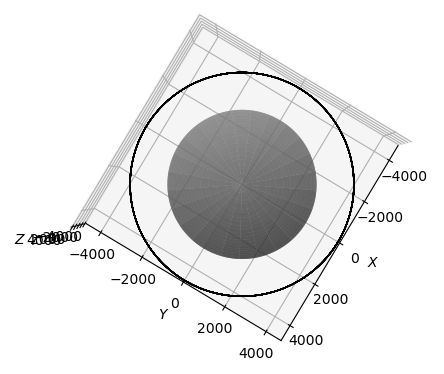
\includegraphics[width=.8\textwidth]{Im/luz_circular.png}
    \caption{Órbita circular}
\end{figure}

\begin{figure}[h!]
    \centering
    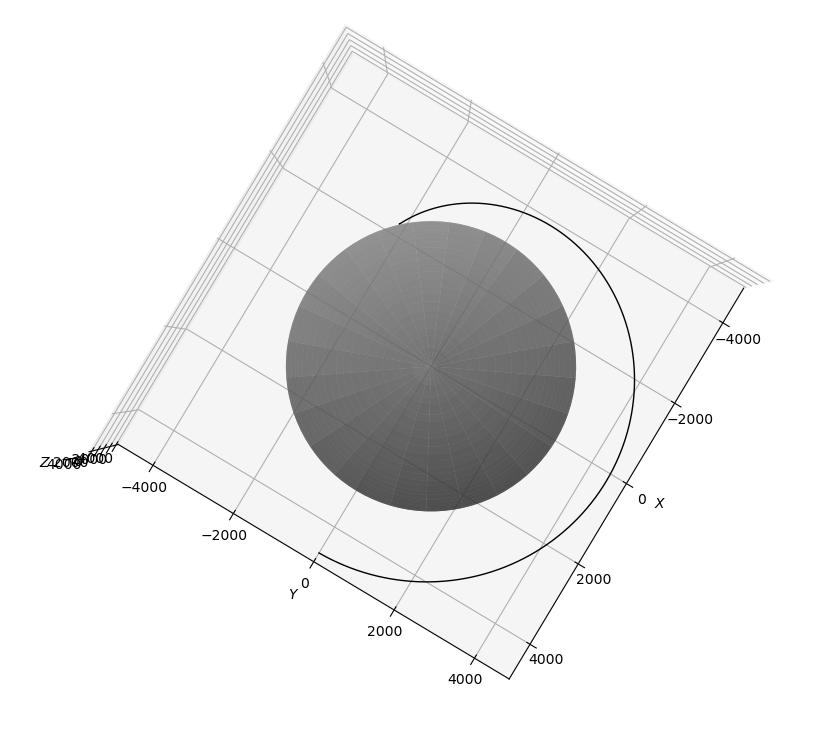
\includegraphics[width=.8\textwidth]{Im/luz_interior_angulo91.png}
    \caption{Desviación de 1° la órbita circular hacia el interior}
\end{figure}

\begin{figure}[h!]
    \centering
    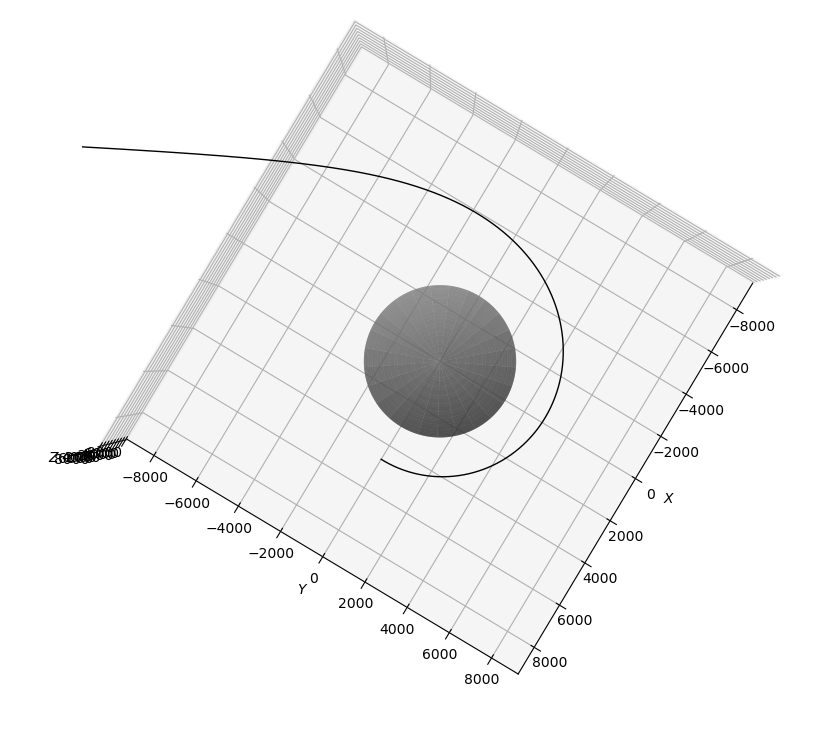
\includegraphics[width=.8\textwidth]{Im/luz_exterior_angulo89_1vuelta.png}
    \caption{Desviación de 1° de la órbita circular hacia el exterior}
\end{figure}

\newpage
\subsection*{\textbf{Órbita de Mercurio}}
Uno de los grandes problemas que tuvo la Mecánica Newtoniana es explicar las observaciones respecto a la precesión del perihelio de Mercurio: La teoría predecía una precesión de $531.9\ arc seg/siglo$, mientras que las observaciones medían $575\ arc seg/siglo$ ¡Una diferencia de $43\ arc seg/siglo$! Pasaron décadas hasta que al fin la teoría de la Relatividad General de Einstein mostró que al considerar la curvatura del espacio-tiempo debido al sol, Mercurio precesa aproximadamente $43\ arc seg/siglo$. Y, añadiéndole la contribución de los otros planetas del sistema solar se termina de explicar las observaciones. Simulamos una partícula partiendo del perihelio de mercurio, moviéndose con velocidad radial nula y velocidad tangencial máxima. Las condiciones iniciales\footnote{https://nssdc.gsfc.nasa.gov/planetary/
factsheet/mercuryfact.html} son:
\begin{equation}
    r_{inicial}=46.002x10^6 Km\ \text{, }\ \Vec{V}= 0\Vec{e}_r + (58.98 m/s)\Vec{e}_{\phi}
\end{equation}

\begin{figure}[h!]
    \centering
    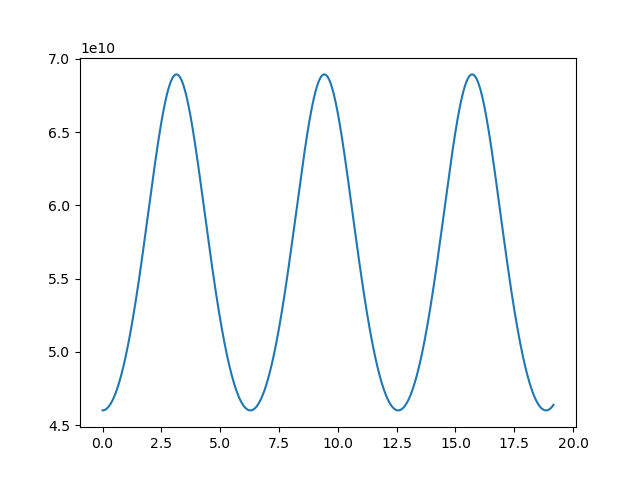
\includegraphics[width=.8\textwidth]{Im/rvsphi_mercurio.png}
    \caption{Gráfica de la órbita de Mercurio: $r$ vs $\phi$}
\end{figure}

Midiendo a que ángulos se dan los mínimos, los perihelios, y viendo la diferencia de esos ángulos se puede estimar la precesión del perihelio. Con la precisión que tenemos, este número nos varía entre la mitad del valor real, y el doble del valor real. 

\begin{figure}[h!]
    \centering
    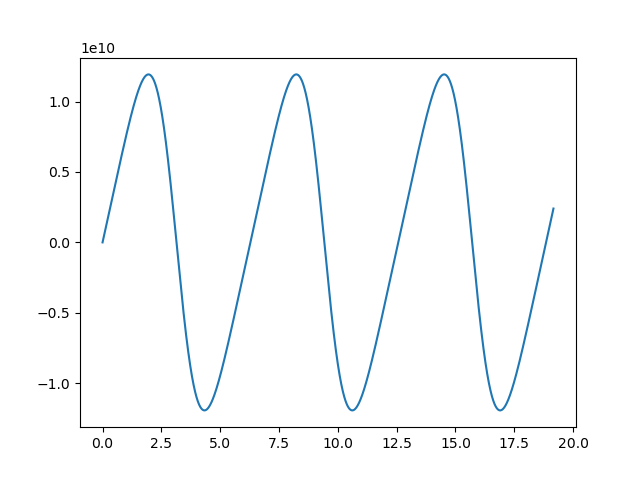
\includegraphics[width=.8\textwidth]{Im/drvsphi_mercurio.png}
    \caption{Gráfica de $\frac{dr}{d\phi}$ vs $\phi$}
\end{figure}

\subsection*{Muchas posibilidades}
Bajo ciertas limitaciones computacionales, es posible jugar con cualquier condición inicial. Dejamos una genial:

\begin{figure}[h!]
    \centering
    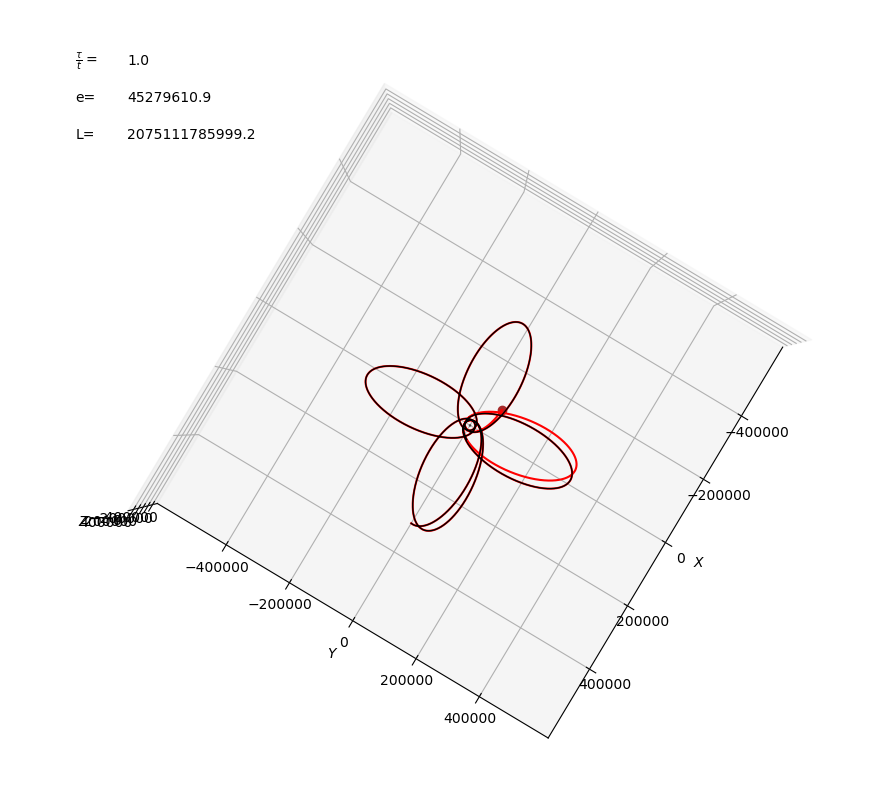
\includegraphics[width=.8\textwidth]{Im/Roseta.png}
    \caption{Órbita divertida en forma de flor.}
\end{figure}
\newpage


%Simulations
%\chapter*{\textcolor{myred}{Epílogo}}

\textcolor{black}{\hrule}
\vspace{0.5cm}
{\huge{Conclusiones y Fronteras}}
\vspace{0.5cm}
\textcolor{black}{\hrule}

\newthought{Luego de haber realizado todo este recorrido por agujeros negros y espacio-tiempos curvados}, podemos afirmar que hemos aprendido mucho sobre Relatividad General. Ya sabemos interpretar muchas ecuaciones y métricas, e incluso hallar nuestras propias métricas para sistemas nuevos.

\vspace{0.5cm}

Uno de los resultados más interesantes a los que llegamos, que contradice bastante lo que estudiamos en Física III y Electromagnetismo I y II, es que aquí \textbf{los objetos con carga modifican las trayectorias de cualquier tipo de partícula}, independientemente de si esta última tiene carga o no. Esto es porque la fuente de la curvatura del espacio-tiempo es la \textbf{energía} (tensor de estrés-energía). Que un objeto sin carga pueda interactuar con un objeto con carga es un resultado análogo (e igual de sorprendente) a cuando un objeto sin masa -la \textbf{luz}- interactúa con un objeto con masa.

\vspace{0.5cm}

También fuimos capaces (no sin dificultad) de desarrollar un programa que realiza simulaciones de las trayectorias de partículas en un espacio-tiempo de Reisser-Nordström. Como esto es una generalización de espacio-tiempo de Schwarzschild, el programa también sirve para simular los problemas más conocidos de la Relatividad General: precesión del perihelio de Mercurio, deflección de la luz cerca de un objeto masivo. Incluso pudimos hacer una simulación del Sistema Solar.

\vspace{0.5cm}

Es posible expandir este trabajo realizando un estudio más minucioso del espacio-tiempo cerca del agujero negro de Reissner-Nordström, la presencia de carga eléctrica nos habilita a definir un nuevo radio, denominado \textbf{Radio de Cauchy}, que establece una región nueva entre dicho radio y el horizonte de eventos. Es posible analizar las diferencias entre cada una de las regiones del agujero negro. Este nuevo radio también nos permite postular la existencia de \textbf{singularidades desnudas}, que no tienen horizonte de eventos. Es decir, son agujeros 'negros' \textit{que dejan pasar la luz}.

\vspace{0.5cm}

Los agujeros negros con carga no existen en la realidad: para que los fenómenos aquí estudiados sean apreciables, necesitaríamos una carga del orden de los $10^{18}$ Coulomb. Sin embargo, el interés en este tipo de problemas no es puramente teórico: la métrica de Reissner-Nordström es el primer paso hacia la construcción de una métrica más general, que estudia los agujeros negros que rotan. Esta es la \textbf{métrica de Kerr}. Obviamente, una posible continuación del trabajo aquí realizado debería incorporar los agujeros negros de Kerr (y de Kerr-Newman, que rotan \textit{y} tienen carga eléctrica).

\vspace{0.5cm}

Por último, existe una rama de la Relatividad General llamada \textbf{gravitational lensing}, que estudia cómo la presencia de objetos masivos, al desviar la luz proveniente de estrellas lejanas, modifica las imágenes que pueden observarse desde la Tierra. Esto nos invita a utilizar técnicas computacionales de raytracing para simular cómo se vería un agujero negro.

\begin{figure}
    \centering
    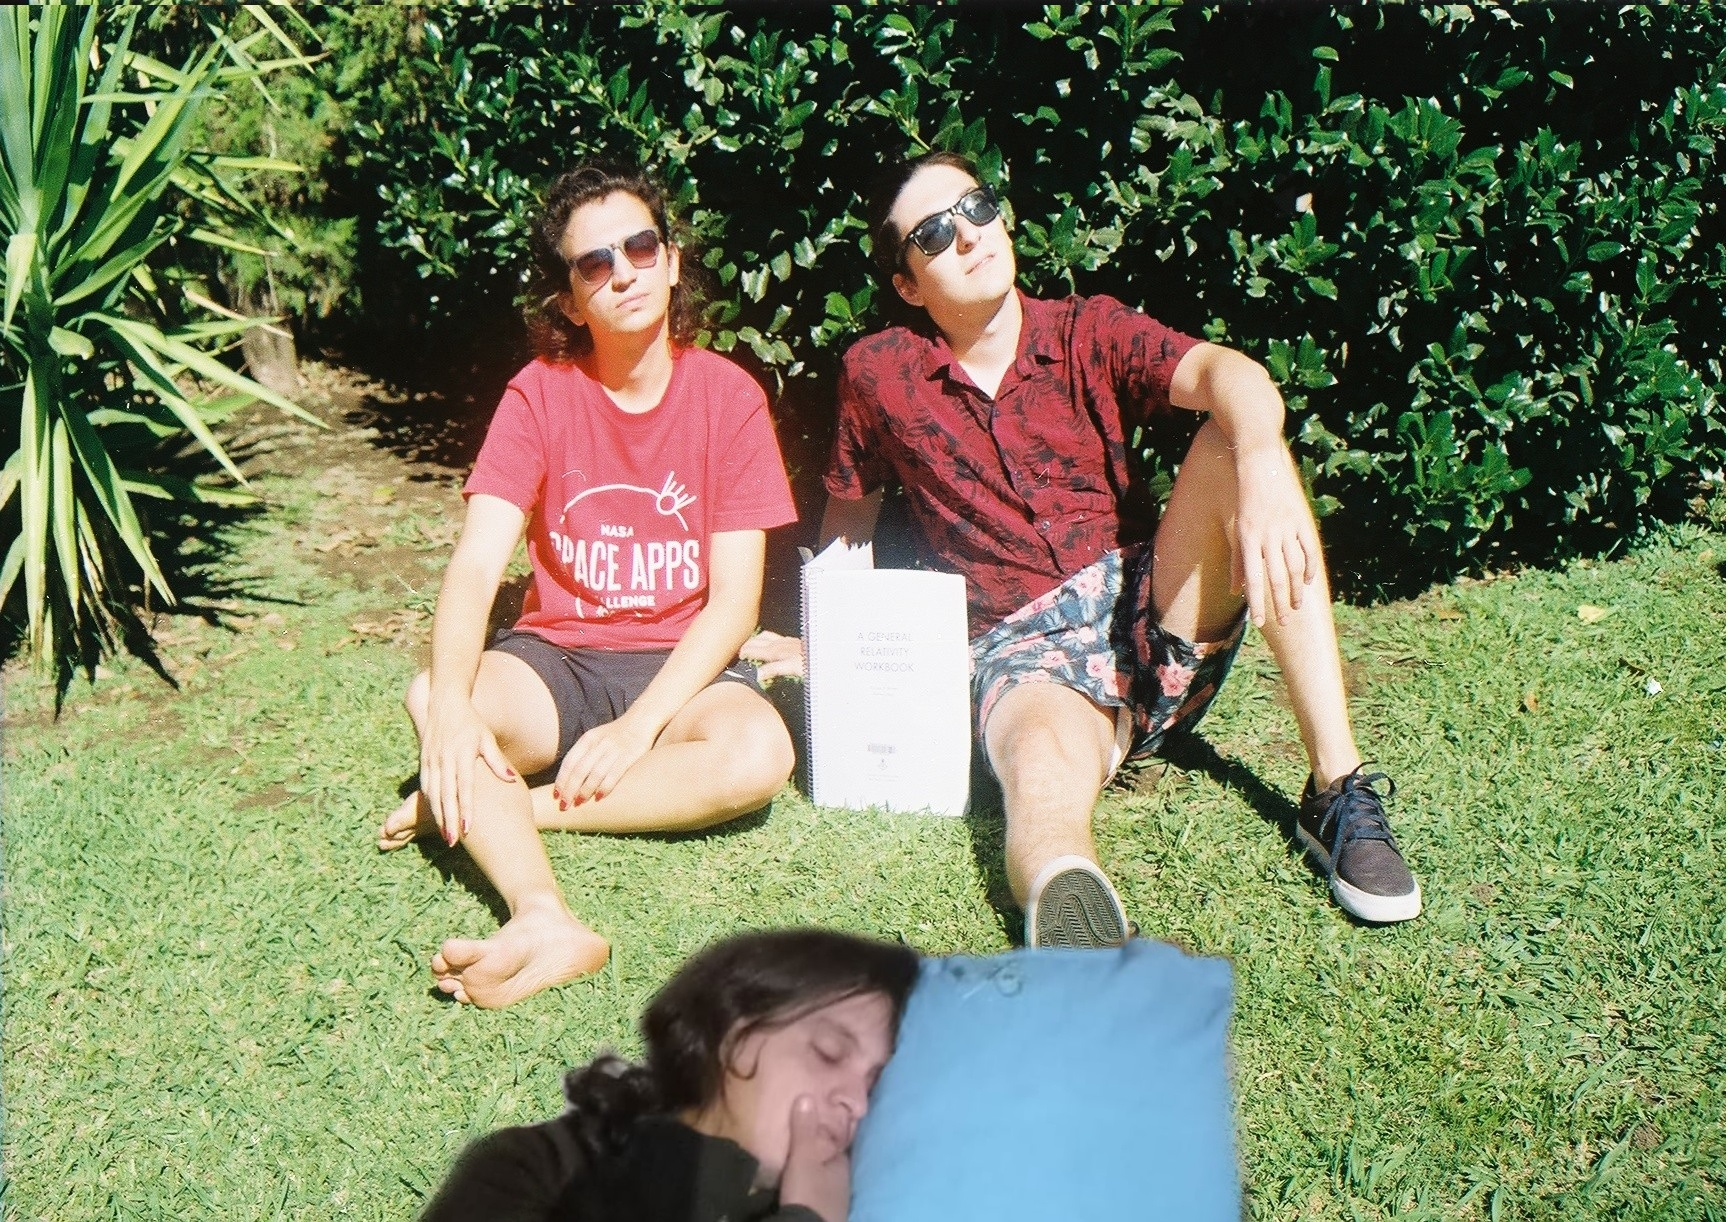
\includegraphics[width=\textwidth]{Im/F1000033-01.jpeg}
    \caption{Amigues relativistas.}
    \label{fig:my_label}
\end{figure}

\newpage
\textcolor{black}{\hrule}
\vspace{0.5cm}
{\huge{Material de Estudio}}
\vspace{0.5cm}
\textcolor{black}{\hrule}


\newthought{A continuación}, vamos a realizar un breve recorrido por los distintos recursos que utilizamos para estudiar estos temas.

\subsection*{\textbf{A General Relativity Workbook}, de Thomas A. Moore}
Este fue nuestro libro de cabecera, y tal como su nombre lo indica, es un libro diseñado para trabajar. Los capítulos tienen entre 5 y 10 páginas de extensión, y la mitad de los temas que desarrolla son propuestas para que resuelva lx estudiante. Abarca todos los temas relevantes para un primer curso de Relatividad General, y utiliza conceptos claros y sintéticos. 
\begin{marginfigure}
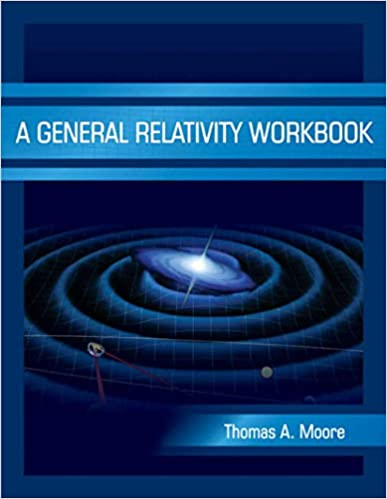
\includegraphics[width=0.8\textwidth]{Im/moore.jpg}
\end{marginfigure}

El libro no deja ningún término matemático sin definir, lo cual es ideal para quienes necesitan ver las cuentas para terminar de asimilar un tema (como nosotrxs). Es muy útil como guía conductora, aunque a veces no indaga tanto en lo conceptual para \textit{sacarle el jugo} a los temas.

\subsection*{\textbf{Exploring Black Holes: An Introdution to General Relativity}, de John A. Wheeler y Edwin F. Taylor}

Si en libro anterior tenía mucha matemática y poca interpretación, este libro es todo lo contrario. Sin mencionar tensores ni diferenciación covariante en ningún momento, los autores proponen trabajar con métricas 'dadas' y estudiar al máximo (\textit{explorar}) cómo es la geometría del espacio-tiempo. 
\begin{marginfigure}
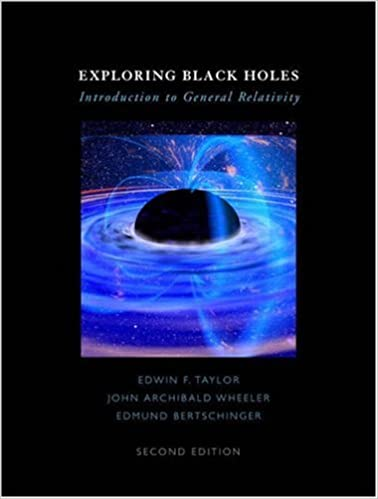
\includegraphics[width=0.8\textwidth]{Im/wheeler.jpg}
\end{marginfigure}
De a ratos puede parecer que todo está un poco \textit{en el aire}, en especial para quienes, al igual que nosotrxs, prefieren libros un poco más matemáticos. 

Algo muy interesante es la cantidad de proyectos que propone el libro. De hecho, la mitad del libro son instrucciones muy detalladas para resolver dichos proyectos. Fue el primer libro que encontramos sobre RG, porque justamente estábamos buscando proyectos guiados para resolver.

\subsection*{\textbf{The Classical Theory of Fields}, de Landau y Lifshitz}


Este libro no requiere demasiada introducción: para algunas personas es un \textit{ladrillo}, mientras que para otras es una \textit{caricia al alma}. 
\begin{marginfigure}
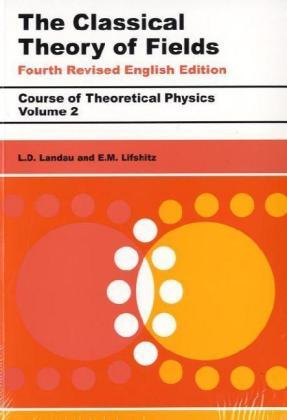
\includegraphics[width=0.8\textwidth]{Im/landau.jpg}
\end{marginfigure}
Lo cierto es que es un libro ideal para agarrar una vez que ya manejamos un poco los temas (lo mismo sucede con todos los libros de la serie de Landau), ya que no se priva de nada: tiene todo el formalismo matemático correspondiente a RG \textit{y} es conceptualmente profundo.
Sin dudas es un buen libro para consultar dudas, y en los primeros capítulos nos sirvió para tomar un hilo conductor.

\newpage

\subsection*{\textbf{Clases de Stanford} de Leonard Susskind}

Esta serie de 10 clases es ideal para ver los alcances que tiene la RG, explicados por una persona que lleva muchos años en el tema.
\begin{marginfigure}
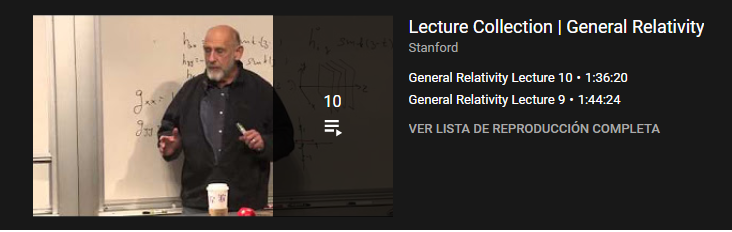
\includegraphics[width=1.3\textwidth]{Im/susskind.png}
\end{marginfigure}
Creo que se pueden apreciar mejor después de haber leído los capítulos 3 a 6 y 17 a 19 del Moore, ya que Susskind casi no escribe en el pizarrón y a veces es difícil seguir los conceptos matemáticos más abstractos sin una buena representación visual. Es ideal para estudiar qué sucede en un agujero negro de Schwarzschild y para introducirse en los Diagramas de Penrose.

\subsection*{\textbf{Einstein Field Equations For Beginners!} de DrPhysicsA}

Este video es la manera perfecta de spoilearse RG desmenuzando las Ecuaciones de Einstein. Todo el video está hecho en una hoja de papel y narrado por una voz con un acento muy inglés. 
\begin{marginfigure}
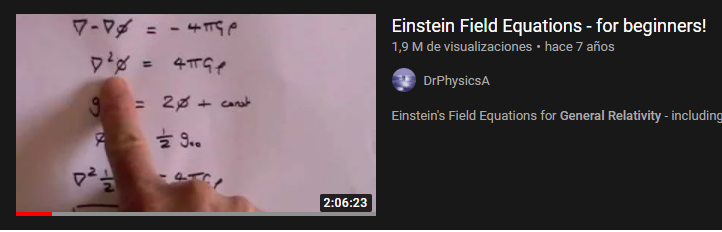
\includegraphics[width=1.3\textwidth]{Im/bumpyy.png}
\end{marginfigure}
Creo que es una buena manera de hacer un pantallazo general de los temas, ya que es muy fácil de entender y nos presenta todos los elementos que vamos a tener que utilizar más adelante.

\subsection*{\textbf{Your Daily Equation} de Brian Greene}

A partir del episodio 26, el autor de \textbf{The Elegant Universe} comienza a explicarnos las Ecuaciones de Campo de Einstein y todos los elementos que la constituyen.
\begin{marginfigure}
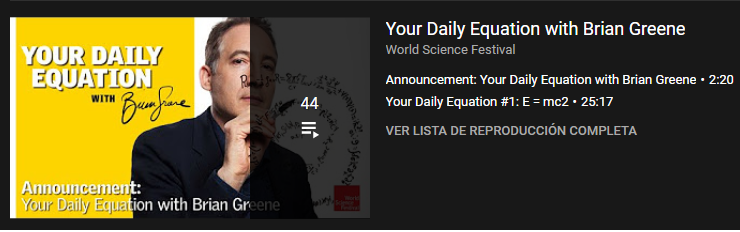
\includegraphics[width=1.3\textwidth]{Im/bumpy.png}
\end{marginfigure}
Da muchos ejemplos para hacer entender los conceptos, y de ahí sacamos gran parte de la sección \textit{GR In a Nutshell} de este apunte.

\subsection*{\textbf{The Maths of General Relativity} de Science Clic}

Esta es una serie de 8 videos que empezó a subirse a finales de 2020 y fue terminada en enero de 2021. Las animaciones están muy bien hechas y permiten entender varios conceptos de manera rápida y clara. 

Se complementa muy bien con libros como el Moore o el Landau, ya que en una animación de 15 segundos sintetiza lo que Landau puede estar dos páginas enteras explicando sin usar una sola imagen.
\begin{marginfigure}
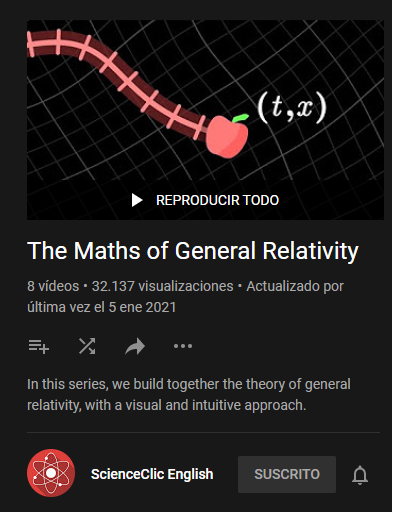
\includegraphics[width=1.3\textwidth]{Im/scienceclic.png}
\end{marginfigure}

\begin{marginfigure}

\includegraphics[width=0.8\textwidth]{Im/qr_img.png}
\end{marginfigure}
\vspace{4cm}
\newthought{En el siguiente link}, encontrarán toda información relacionada con este trabajo, así como también los códigos que hicimos para realizar las simulaciones y varios videos de dichas simulaciones.

\textcolor{myred}{\underline{\url{https://drive.google.com/drive/folders/1AZ_T-1sP442UiVBRkR45JsUwid0Mn6Qu?usp=sharing}}}





\end{document}